


\documentclass[english,a4paper,titlepage,12pt]{report}

%\usepackage{glossaries}
%\usepackage{harvard}
\usepackage{natbib}
\bibliographystyle{agsm}
% \usepackage{harvard}
 %\usepackage[dcucite]{harvard} 
\usepackage{a4wide}
\usepackage{aas_macros}
\usepackage{sidecap}
%\usepackage{agsm}
%\usepackage{jjastron}
%\bibliographystyle{justin}
%\bibliographystyle{}
\usepackage{fancyhdr}
\usepackage{chronology}
\usepackage{url}
\usepackage{graphicx}
\usepackage{rotating}
\usepackage{xspace}
\usepackage{tikz}
\usetikzlibrary{decorations}
\usepackage{subfloat}
\usepackage{subfig}
%\usetikzlibrary{snakes} 
\usepackage{colortbl}
\usepackage{setspace}

%\makeglossary





\setlength{\hoffset}{-0.5in}
\setlength{\headheight}{20mm}
\setlength{\voffset}{-0.2in}
\setlength{\textwidth}{17.5cm}
\setlength{\textheight}{21cm}
\setlength{\headwidth}{\textwidth}

\renewcommand{\headrulewidth}{0.4pt}
\renewcommand{\footrulewidth}{0.4pt}

\lhead{}
\rhead{}
\chead{\large Thesis.ThesisFinal }

\newcommand{\fign}[1]{Figure~\ref{#1}\xspace}
\newcommand{\eqn}[1]{Equation~\ref{#1}\xspace}
\newcommand{\secn}[1]{Section~\ref{#1}\xspace}
\newcommand{\appen}[1]{Appendix~\ref{#1}\xspace}
\newcommand{\citeasnoun}[1]{\citet{#1}\xspace}
\renewcommand{\cite}[1]{\citep{#1}\xspace}

\newcommand{\controlprogram}[0]{rewritetcp\xspace}
\newcommand{\tcpserver}[0]{tcp\_server\xspace}
\newcommand{\degt}[0]{$^{\circ}$\xspace}
\newcommand{\degc}[0]{$^{\circ}$C\xspace}
\newcommand{\approximately}[0]{$\approx$}
\newcommand{\CMB}{\nomenclature{CMB}{Cosmic Microwave Background}}


\author{Charles Copley\\Hertford College\\University of Oxford}
\title{Thesis.ThesisFinal.git2}
%\college{Hertford College}
%\printglossary
%\addcontentsline{toc}{chapter}{Glossary} % remove this line if you don't want a table of contents entry for the glossary



\begin{document}


%\bibliographystyle{bibfiles/justin.bst}
%\citationstyle{agsm}
\pagestyle{empty}
%\renewcommand\thepage{}
\begin{center}

\begin{figure}[ht]
\centering
\begin{tabular}{ccc}
\begin{minipage}{3cm}

\includegraphics[scale=0.25]{./images/logos/OxfordLogo.png}
\end{minipage}
&
\begin{minipage}{9cm}
\centering
\textbf{\large University of Oxford}
\vspace{1 cm}

\textbf{\large Hertford College}
\end{minipage}
&
\begin{minipage}{3cm}

\includegraphics[scale=0.25]{./images/logos/OxfordLogo.png}
\end{minipage}
\end{tabular}
\end{figure}
\vspace{4 cm}



\textbf{\huge The C-Band All Sky Survey}
\vspace{1 cm}


\textbf{{\large Submitted in fulfillment of the
requirements for the award
of a D.Phil
at the University of Oxford
}}
% \textbf{\Huge }
\vspace{7 cm}
%\textbf{\large A thesis submitted for the degree of}
%\vspace{0.2 cm}

%\textbf{\large Doctor of Applied Sciences}
%\vspace{0.2 cm}

\textbf{\large presented by Charles Copley\\supervised by Professor Michael Jones}
\vspace{1 cm}

\textbf{\today}
\end{center}
\cleardoublepage




%\maketitle
\tableofcontents
\newpage
\pagestyle{fancy}
\doublespace
\begin{abstract}
The C-Band All Sky Survey (C-BASS) is a survey of the sky foreground in both intensity and polarisation at a frequency of 5~GHz with a resolution of $\approx$ 0.8$^{\circ}$. Northern and Southern sky coverage is provided by antennas located at the Owens Valley Radio Observatory (OVRO) in California, and the \textit{Meer}KAT support base in South Africa, respectively.

The primary science goal is to provide a C-Band all sky intensity and polarisation map to augment the WMAP surveys. This lower frequency constraint will allow improved foreground subtraction in Cosmic Microwave Background (CMB) experiments.  Removal of  foregound contamination will place a limit on the success of CMB experiments that attempt to detect the B-Mode polarisation of the CMB. 

This report details the technical developments of the experiment (both North and Southern surveys), the status of the Northern sky survey, and provides details of the new digital receiver being designed and built to deploy on the South African telescope.
\end{abstract}

%\fancyfoot[R]{Page \thepage}

\chapter{Introduction}



\section{Science Goals}

\section{}

\section{Foreground Removal Techniques}

The beginnings CMB polarization studies focused on measuring the relatively bright E-Mode power spectrum. Small area surveys conveniently provided sufficient signal to detect both EE and TE polarization \cite{Leitch2005a,Mcmahon2005,Barkats2005,Readhead2004} , and areas obfuscated by foregrounds were avoided.  Detecting the much fainter B-Mode signals, will require larger area surveys and galactic foreground contamination will be unavoidable \cite{Tegmark2000}. This will require foreground removal.

A number of different foreground removal techniques exist. 


\cite{Hansen2006},\cite{Delabrouille2009},\cite{Leach2008},\cite{ArmitageCaplan2011},\cite{Gold2009},\cite{Dunkley2009},
\section{Survey Requirements}
  \subsection{Beam Size}
  \begin{eqnarray}
   \theta_{HPBW}&\approx& \frac{1.2\lambda}{D}\\
  \theta_{HPBW}&\approx& 0.68^{\circ}\\
   \theta_{HPBW}&\approx& 41''
  \end{eqnarray}

  \subsection{Confusion Limit}
At centimetre wavelengths the confusion noise ($\sigma_{c}$) is observed to be given by
\begin{eqnarray}
 \sigma_{c}&\approx& 0.2 (\nu)^{-0.7}(\theta_{HPBW})^2\\
 \sigma_{c}&\approx& 533mJy/beam
\end{eqnarray}


where the $\sigma_{c}$ is the confusion noise (mJ/Beam), $\nu$ is in GHz and $\theta_{HPBW}$ in arcminutes\\
\url{http://www.atnf.csiro.au/research/radio-school/2011/talks/CondonContinuum2011.pdf}\\
\url{http://www.cv.nrao.edu/course/astr534/Radiometers.html}\\


The confusion limit is about 5$\sigma_{c}$ or $\approx$ 2.5~Jy

 \clearpage
\chapter{Overview of the C-BASS Project}

\cite{Condon}


\section{Northern Antenna}
  \subsection{Optical Configuration}
  Gregorian optical configuration
  \subsection{The Analogue Radiometer/Polarimeter}

  \subsection{Survey Environment}

  \subsection{State of Survey}

\section{Southern Antenna}

  \subsection{Optical Configuration}

  \subsection{The Digital Radiometer/Polarimeter}

  \subsection{State of Survey}

  


 \clearpage
\section{Notch Filters}
\subsection{Radio Frequency Interference (RFI)}

Unfortunately, as the survey has progressed, we have become increasingly beset
by terrestrial, satellite and aircraft interference (see Figure~\ref{fig:intensity}). Aircraft interference is
sporadic enough in nature to flag out, but satellite and terrestrial interference is, however, more troublesome (see \fign{fig:intensity}). The effect on the data is noticeable up to 50$^{\circ}$ elevation, making post-measurement removal very difficult, if not impossible.

 To remedy this on the Northern receiver, we designed a set of narrowband notch filters (to reduce the effect of in-band RFI) and also increased the out-of band attenuation, by adding a second stage of band-defining filters. The resulting change of the passband can be seen in \fign{fig:passbands}. The effect on data quality (\fign{fig:intensityFiltering}) is noticeable and, with the 0.25s/pixel integration period used to produce these scans, RFI is no longer noticeable.

\begin{figure}
 \centering
\subfloat[][The C-BASS pass band before installing any additional filtering]{
 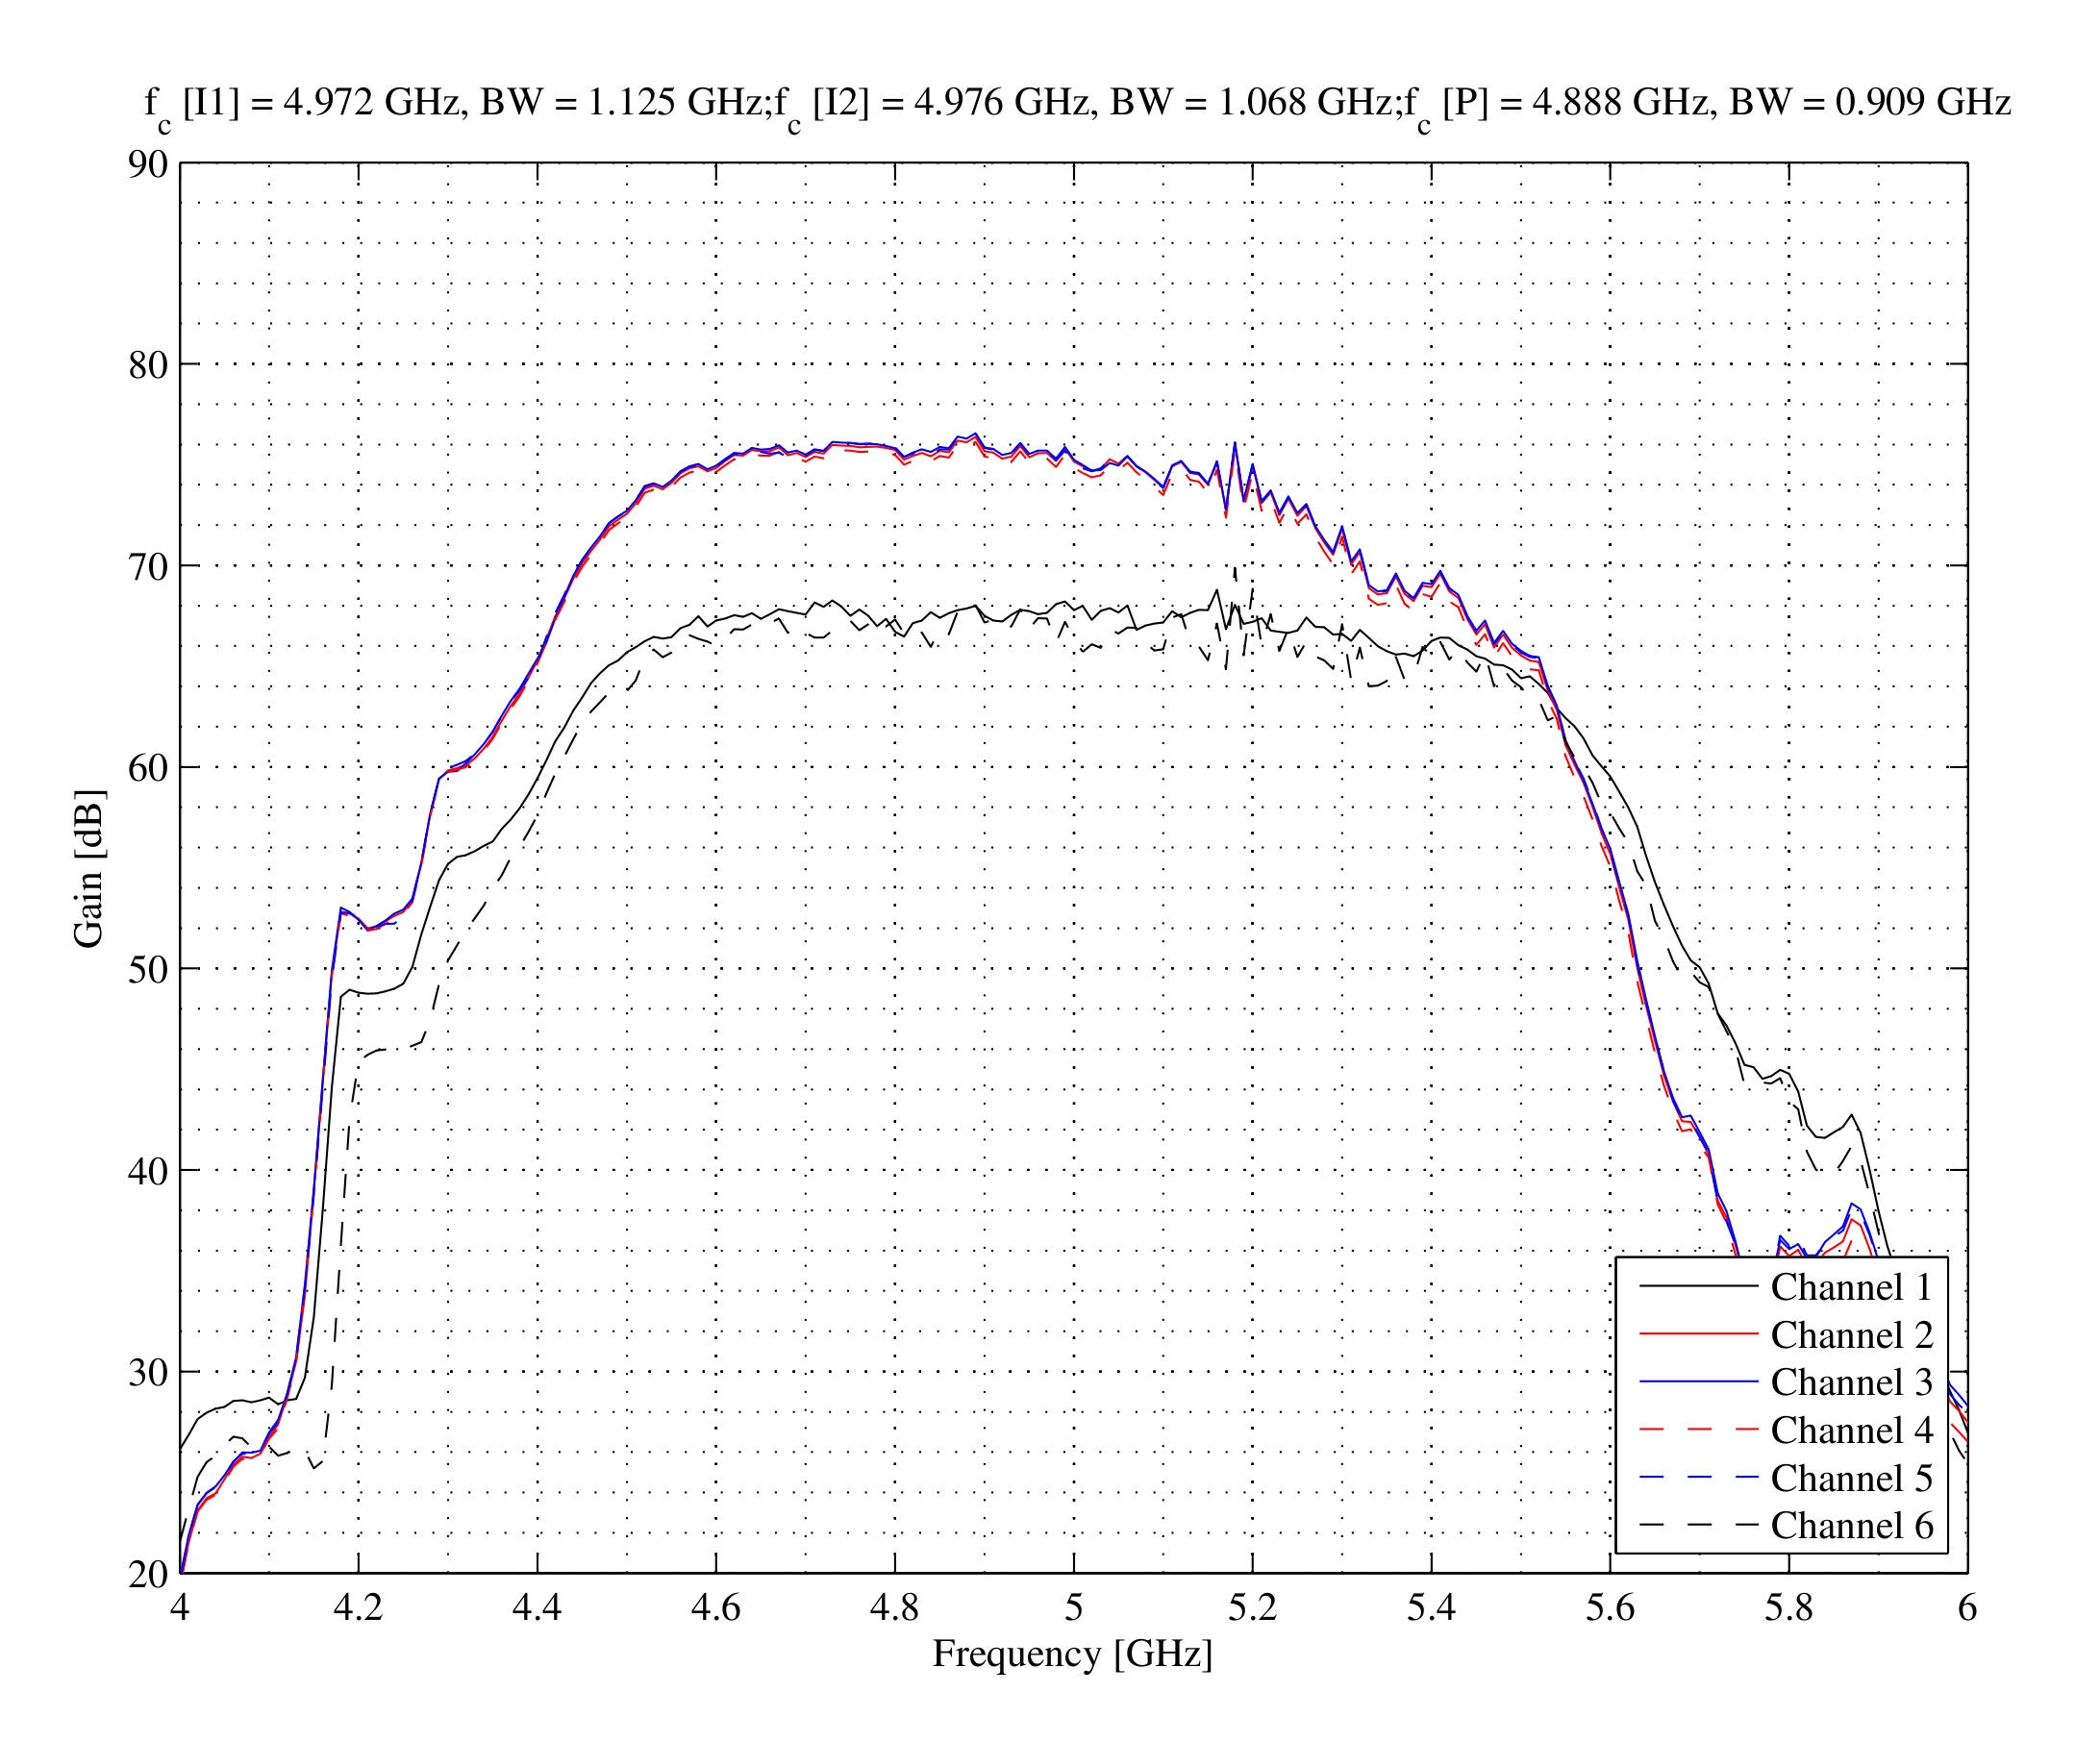
\includegraphics[height=0.4\textheight]{./images/NotchFilter/firstpassband.png}
}\\
\subfloat[][The C-BASS pass band after installing the Notch filters and additional Band pass filters]{
 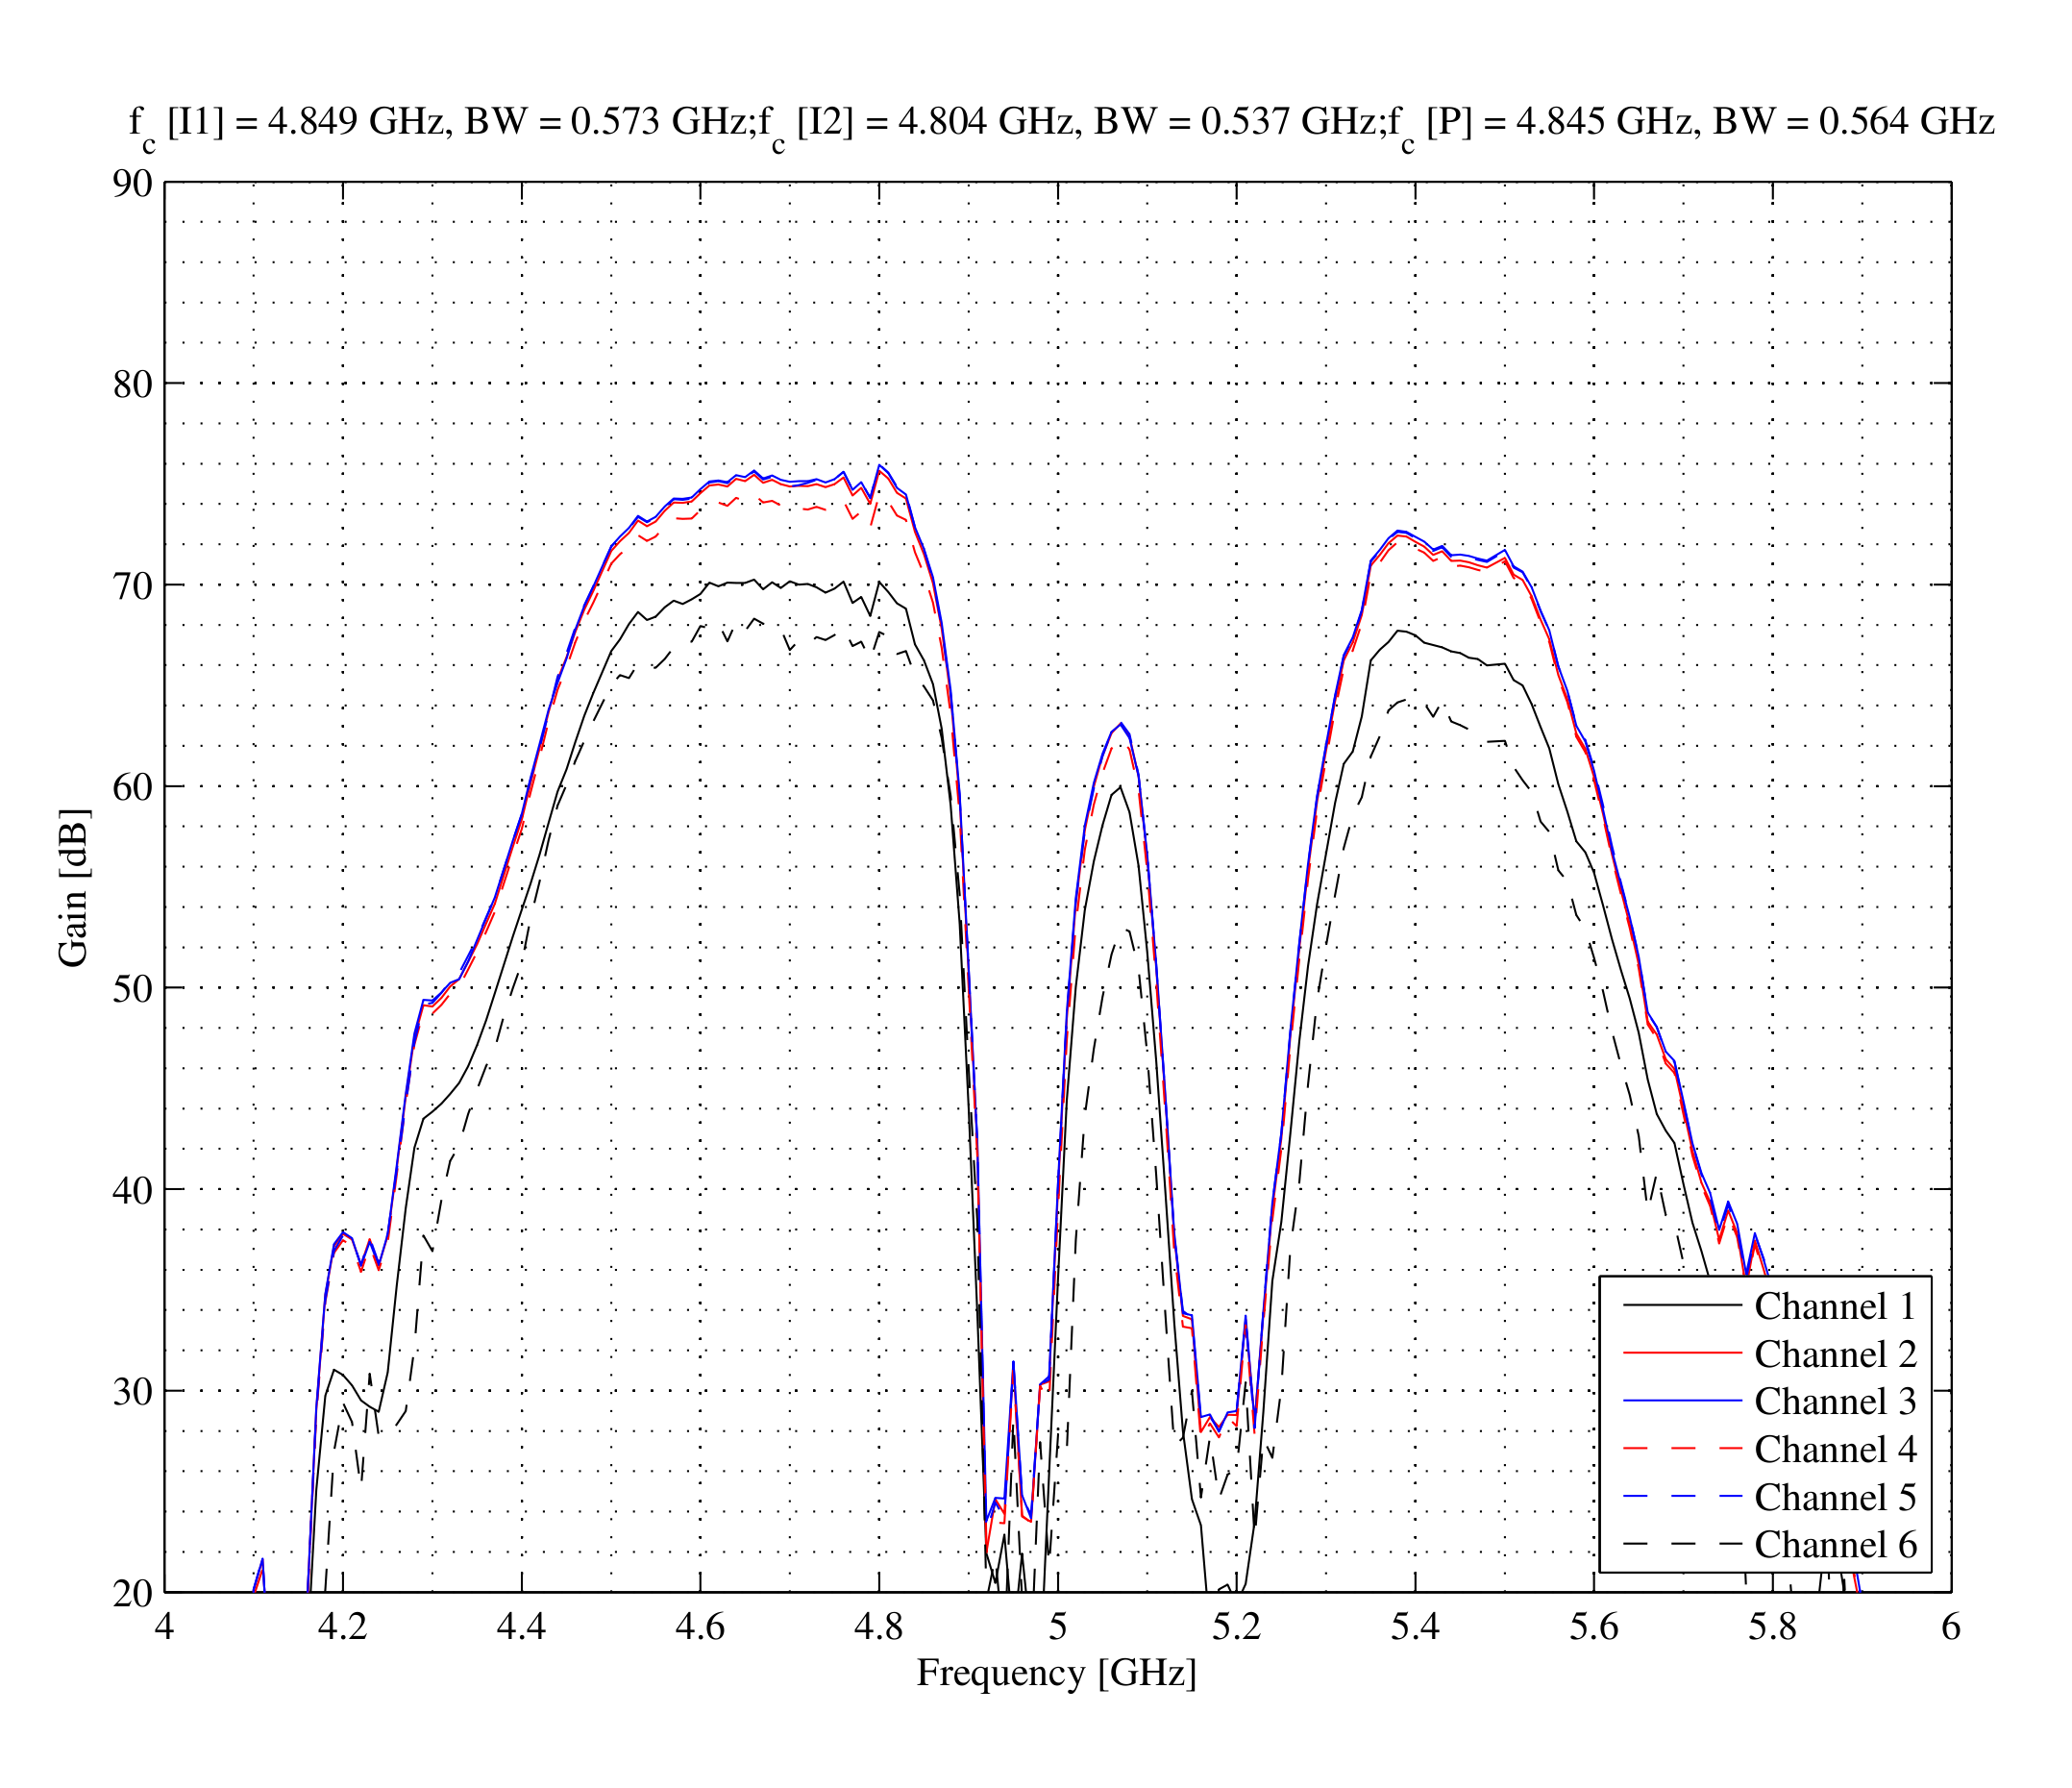
\includegraphics[height=0.4\textheight]{./images/NotchFilter/finalpassband.png}
}
 % firstpassband.pdf: 612x792 pixel, 72dpi, 21.59x27.94 cm, bb=
 \caption{C-BASS passband changes}
 \label{fig:passbands}
\end{figure}

\begin{figure}[ht]
 \centering
 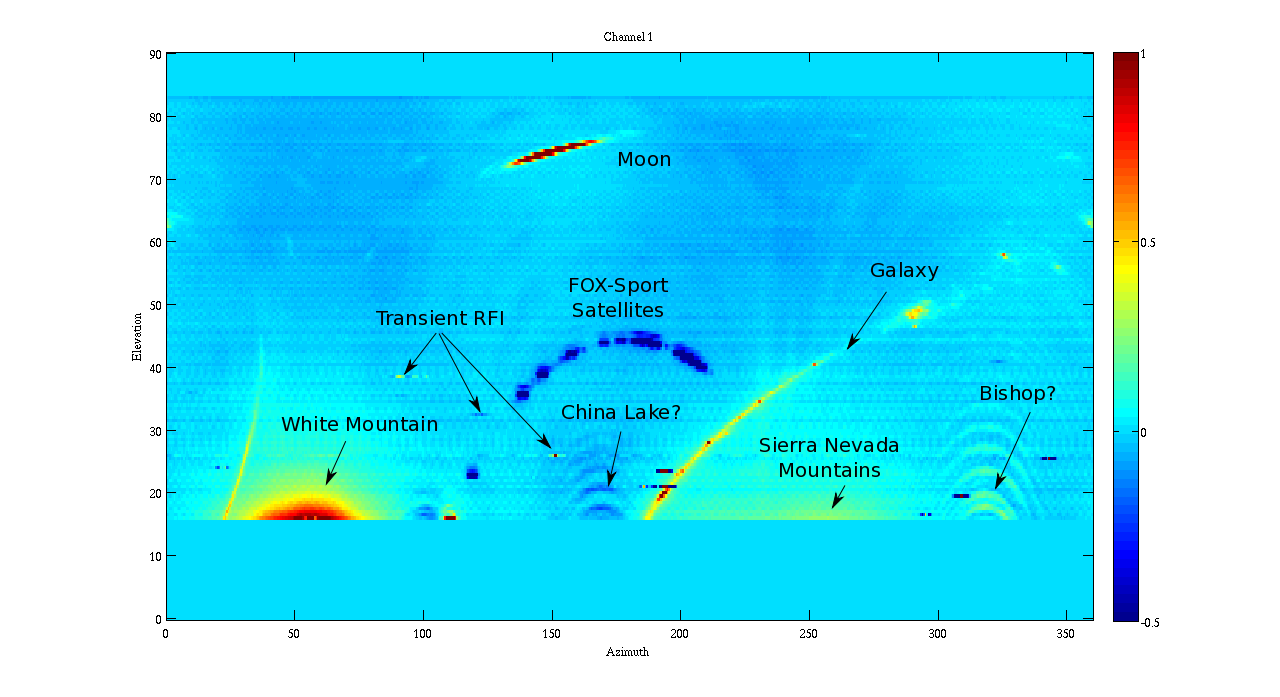
\includegraphics[width=\textwidth]{./images/NotchFilter/altazmapannotated.png}
 % altazmapi.png: 1280x701 pixel, 90dpi, 36.13x19.79 cm, bb=0 0 1024 561
 \caption{Annotated Intensity map (courtesy Oliver) of the sky as seen by the Owens Valley C-BASS antenna. Note the elevation extent of the diffraction patterns seen as a result of the terrestrial radiation }
 \label{fig:intensity}
\end{figure}


\begin{figure}
 \centering
\subfloat[][Sky before the installation of notch filters. Note the diffraction patterns produced by strong RFI sources detected in the antenna sidelobes]{
 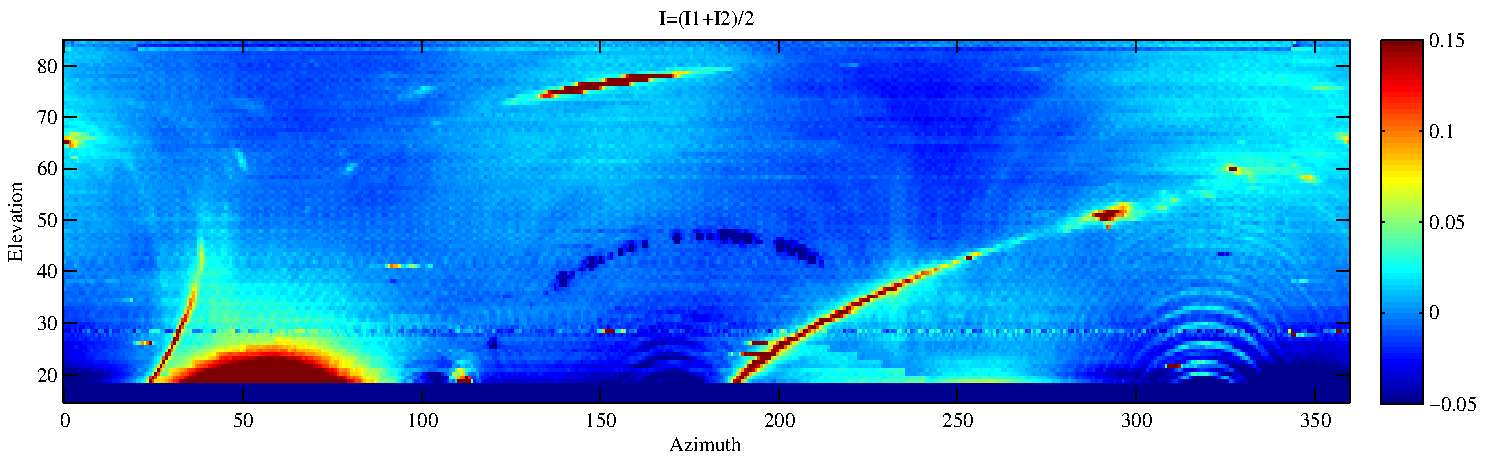
\includegraphics[width=\textwidth]{./images/NotchFilter/IntensityChannelBeforeNotch.pdf}
}\\
\subfloat[][Sky after the installation of notch filters. All terrestrial RFI aside from a strong source to the South ($180^{\circ}$~Azimuth) has been removed ]{
 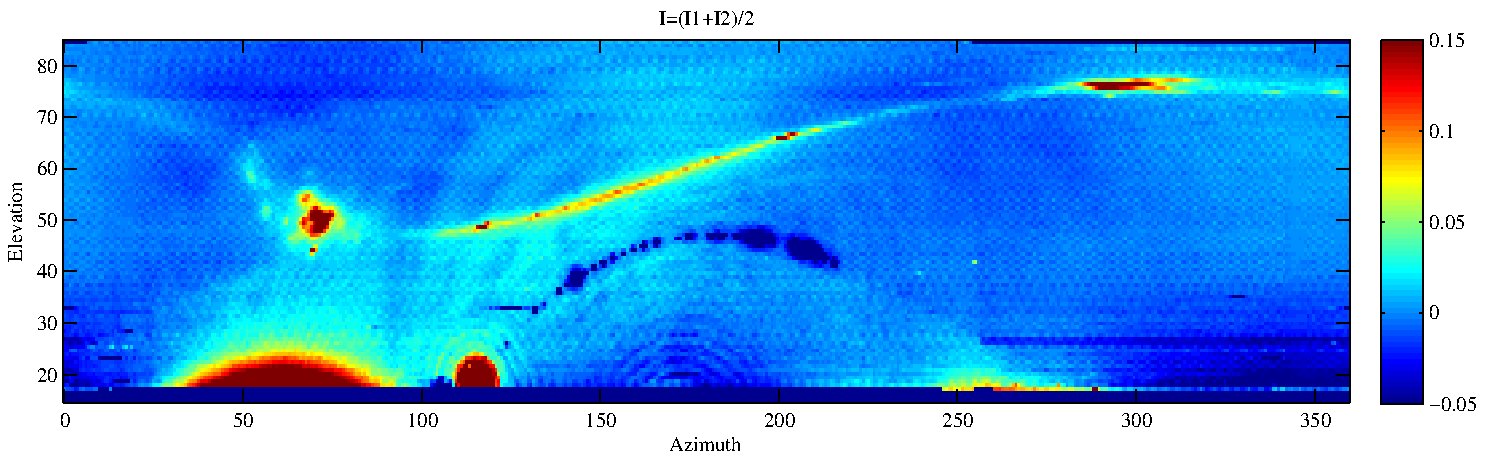
\includegraphics[width=\textwidth]{./images/NotchFilter/IntensityChannelAfterNotch.pdf}
}\\
\subfloat[][Sky after the installation of notch filters and additional band pass filters. All terrestrial radiation removed, and geostationary satellites are no longer visible]{
 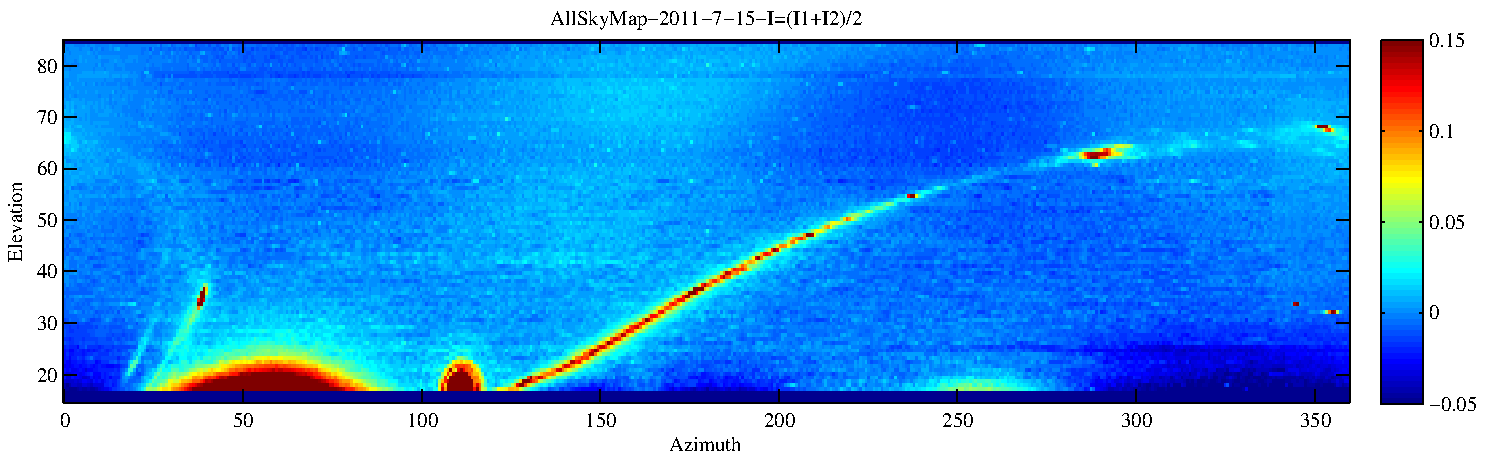
\includegraphics[width=\textwidth]{./images/NotchFilter/IntensityChannelAfterBPFandNotch.pdf}
}
\caption{Installing additional filtering: These images show the dramatic improvement in data quality brought about by the addition of notch filters and additional band defining filters in the C-BASS RF path}
\label{fig:intensityFiltering}
 % IntensityChannelBeforeNotch.pdf: 713x220 pixel, 72dpi, 25.15x7.76 cm, bb=
\end{figure}


\begin{figure}
 \centering
\subfloat[][Radio Frequency Interference as captured by a spectrum analyser attached to the output of the C-BASS cryostat. We think the 4.79~GHz spike is sporadic and does not require filtering]{
 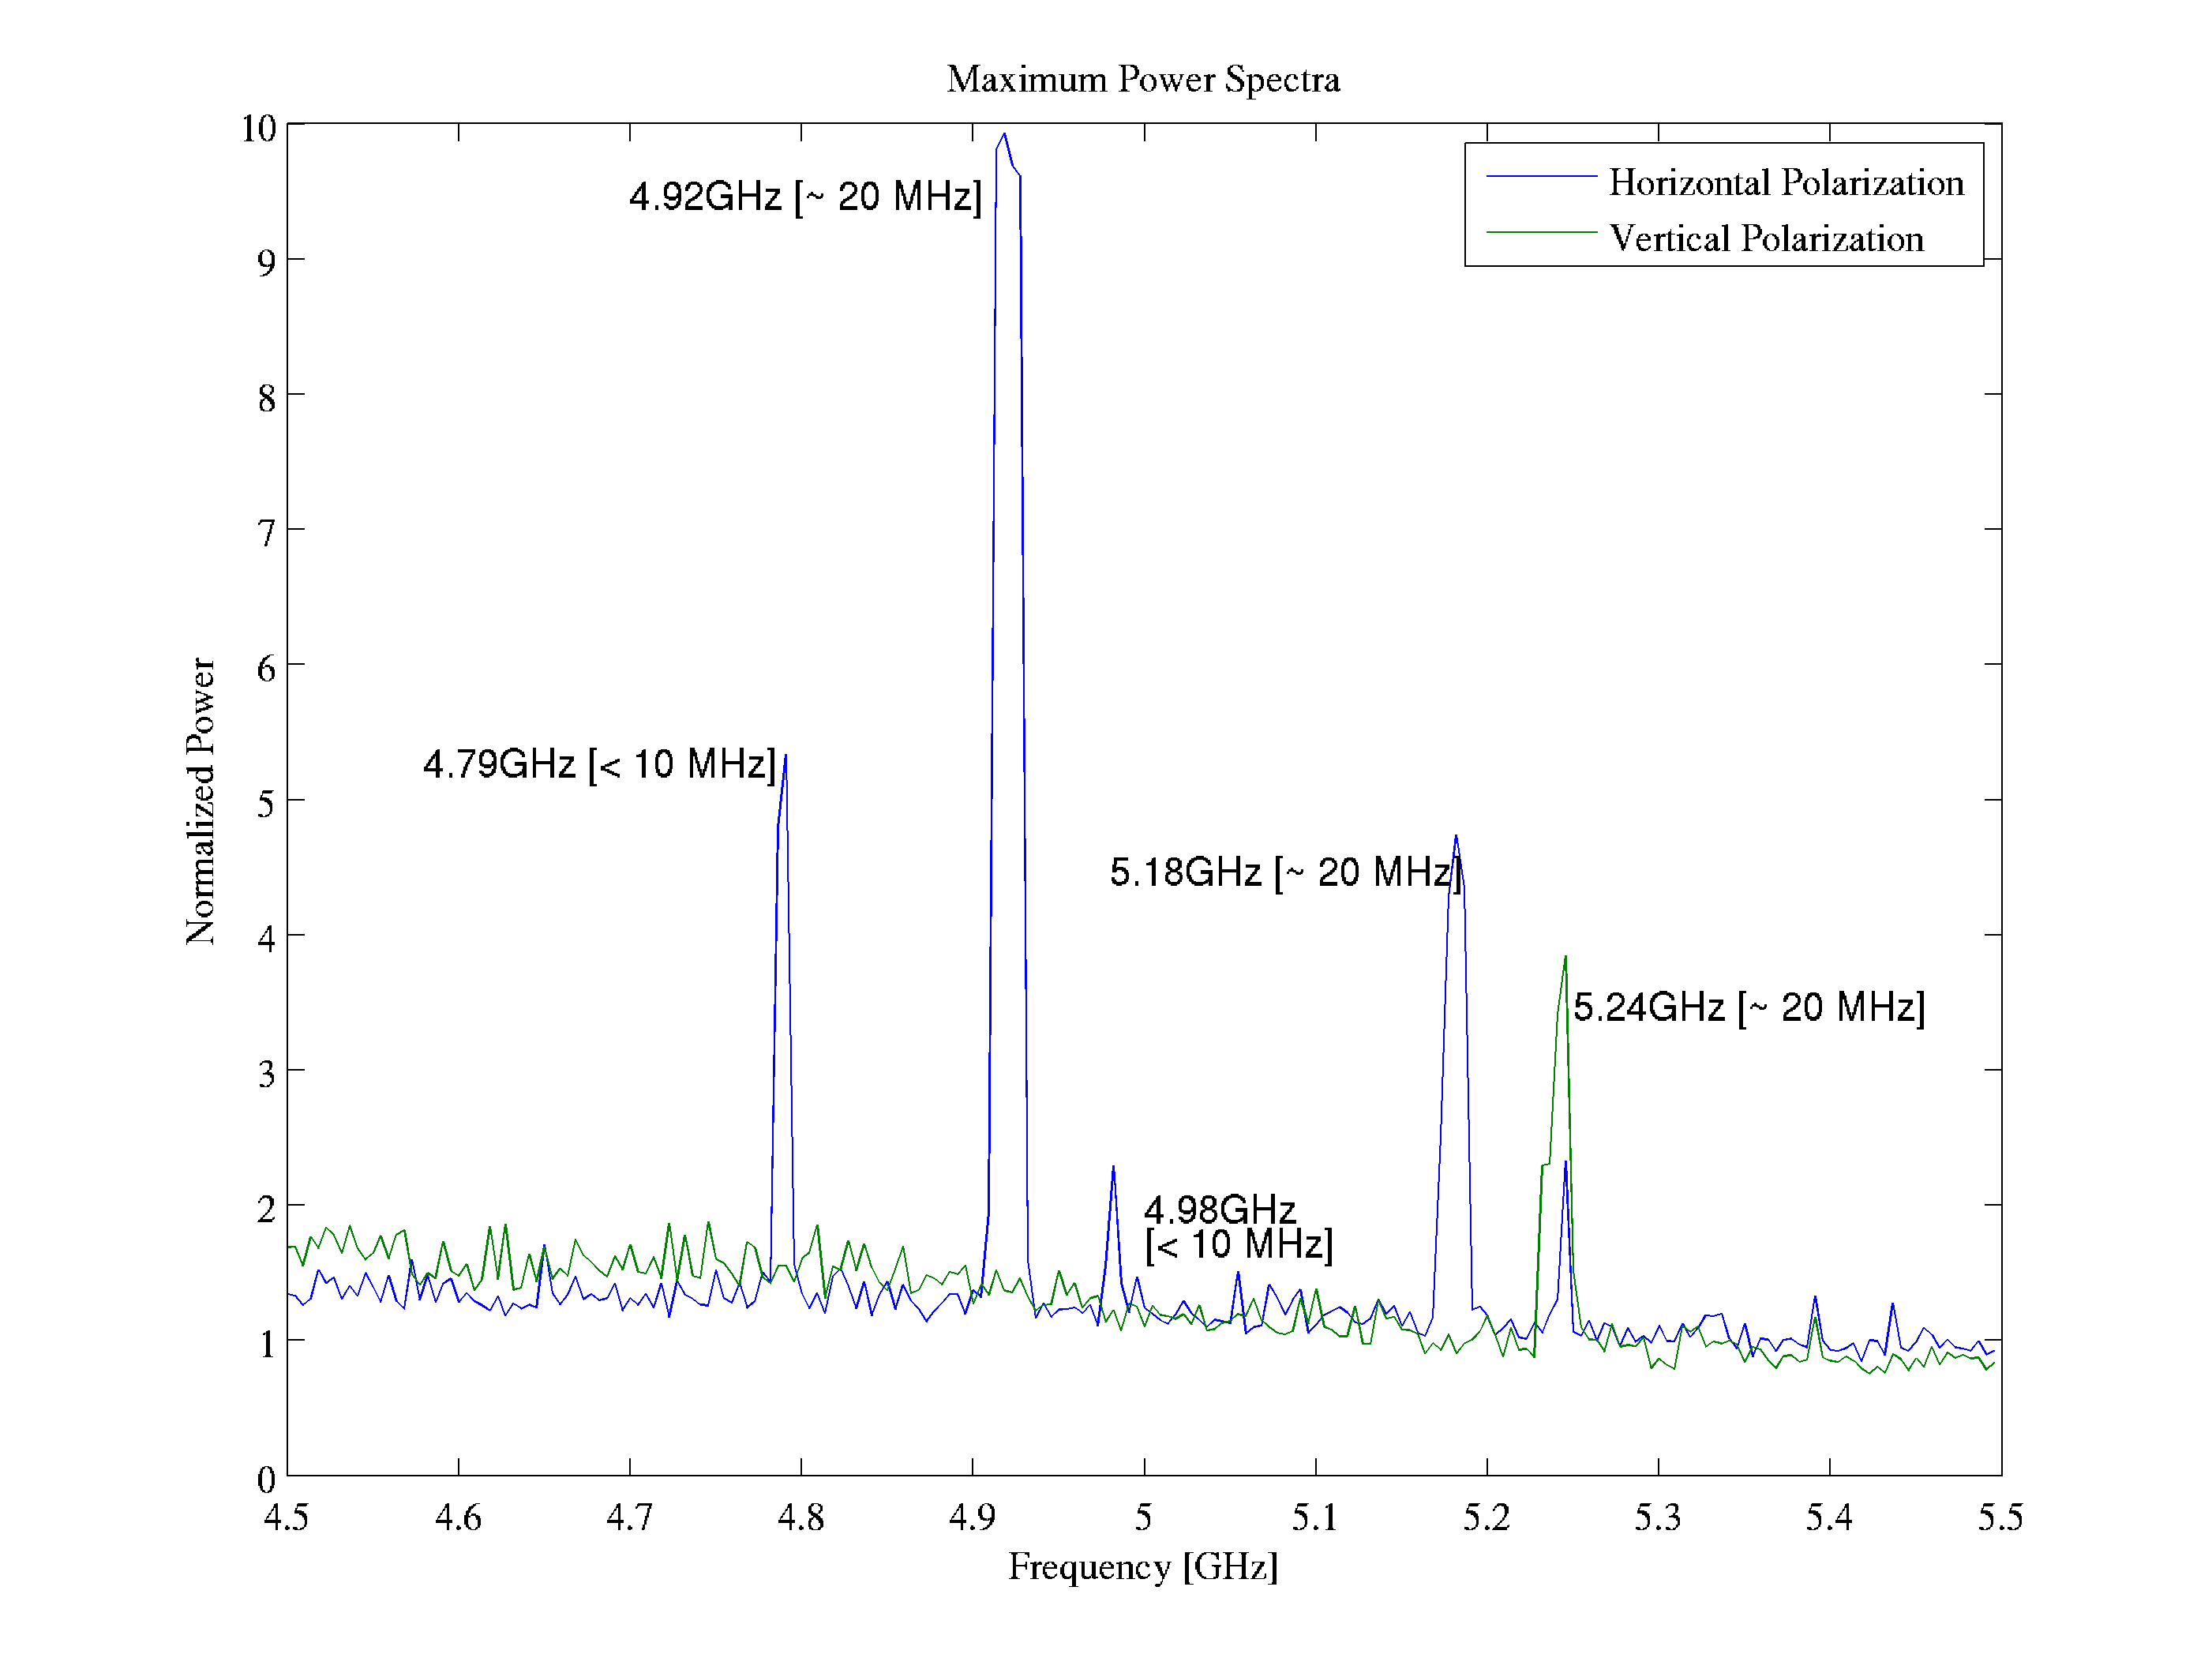
\includegraphics[height=0.4\textheight]{./images/NotchFilter/RFI/norm_max_rfi.png}
}\\
 % norm_max_rfi.png: 2802x2100 pixel, 350dpi, 20.33x15.24 cm, bb=0 0 576 432
 \subfloat[][Spectra of geostationary satellites]{
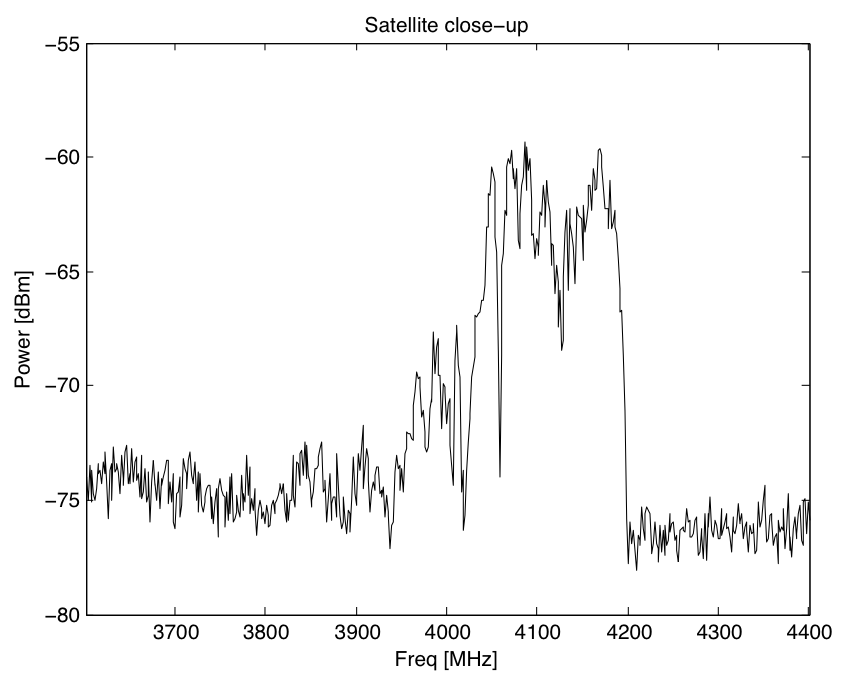
\includegraphics[height=0.4\textheight]{./images/NotchFilter/RFI/figs-satellite.png}}
\caption{}
 \label{fig:RFImaxHold}
\end{figure}




\clearpage
% \begin{figure}
%  \centering
%  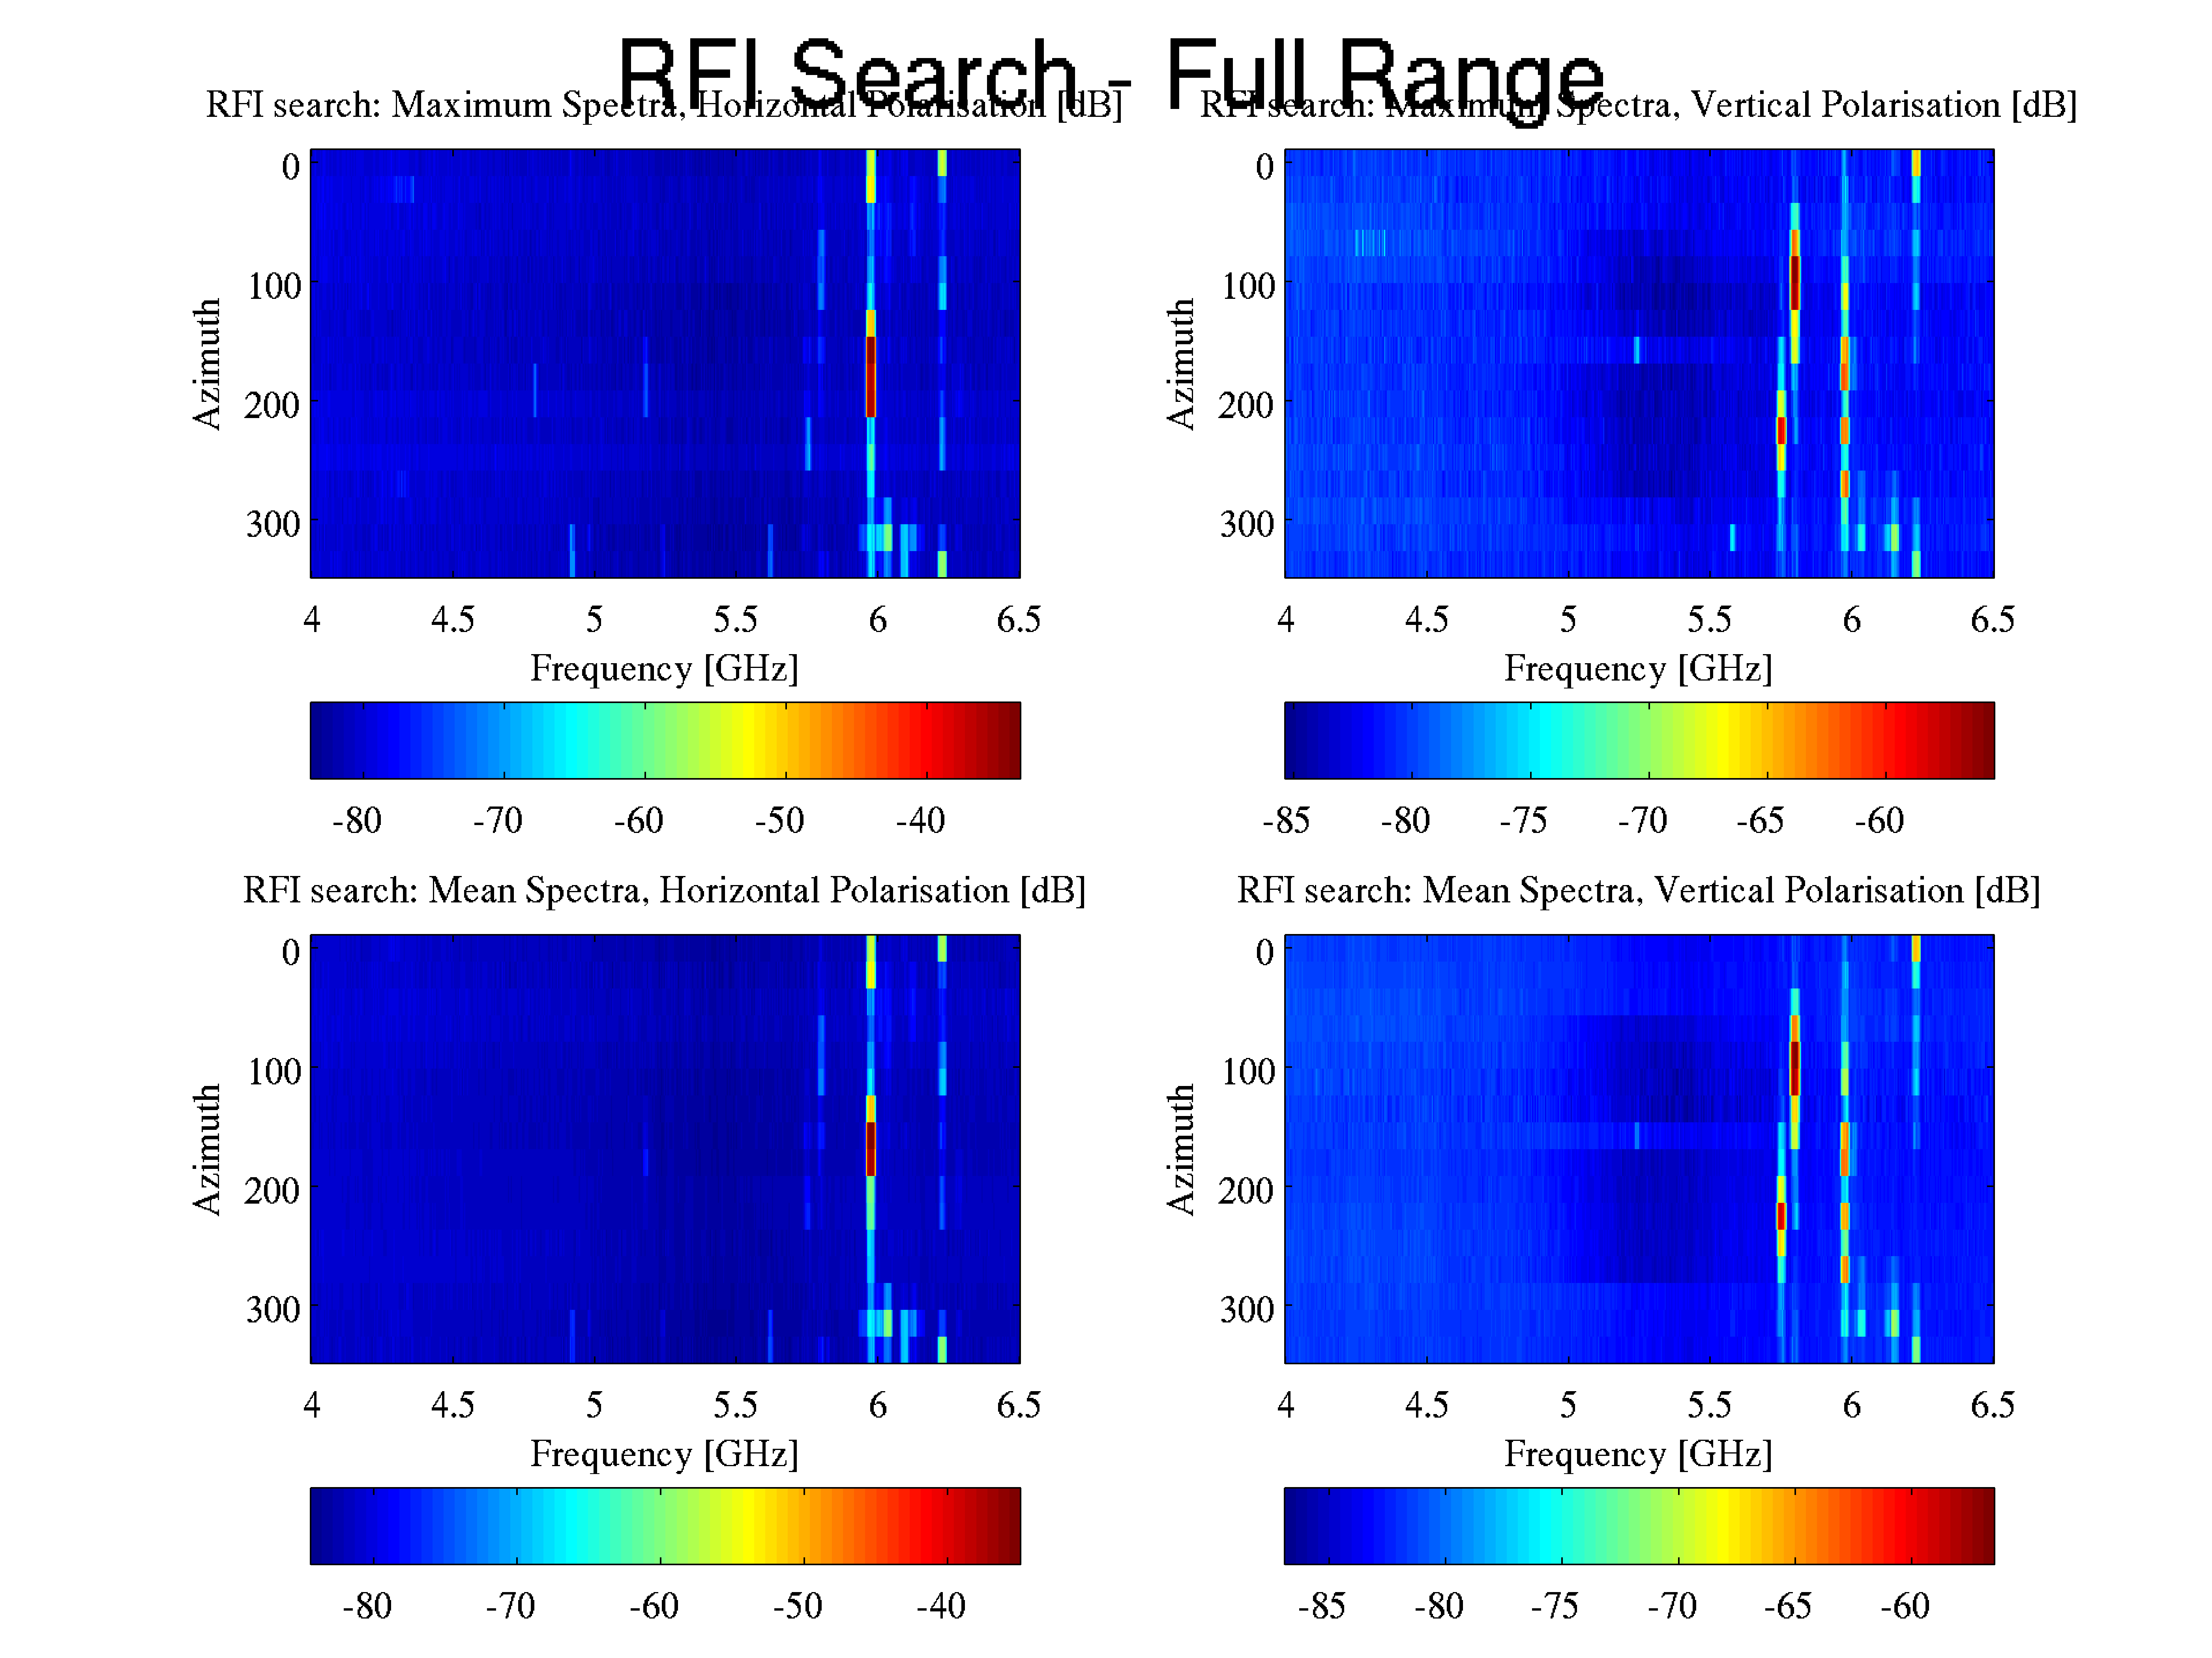
\includegraphics{./images/NotchFilter/RFI/rfi_full_range.png}
%  % rfi_full_range.png: 5605x4200 pixel, 700dpi, 20.34x15.24 cm, bb=0 0 577 432
%  \caption{Radio Frequency Interference as seen at Owens Valley with directionality}
%  \label{fig:RFI}
% \end{figure}


\subsection{Filter Design}

\subsection{Specifications}
An obvious solution to this is to design a set of very high Q ($Q=\frac{f_{c}}{\Delta f}$) notch filters. A cursory examination of Figure~\ref{fig:RFImaxHold} suggests that each RFI band is approximately 25~MHz wide, which at 5~GHz requires a Q of 200. This is a challenging task.

However upon more careful examination of Figure~\ref{fig:RFImaxHold}, it is clear that some relaxation of this is possible. Each of the major RFI bands (i.e 4.92~GHz and 5.18~GHz) has a second proximate RFI peak, which could be included into a single notch filter. To attenuate both of these a stop band of ~80~MHz is required. This is an achievable goal.

\subsection{Design}

High Q filter design using microstrip, is usually accomplished using resonance structures placed parallel to a microstrip transmission line, with electromagnetic coupling between the two. The dimensions of these structures can be adjusted to resonate at the frequency of interest. Alternatively band pass filters can be constructed in a similar fashion by placing these resonating structures in series with the transmission line.

Since this was our first foray into the world of resonance filter designs we looked for a simple resonating structure which would be easy to 'tune'. The design we chose \cite{Garcia2005} is shown in Figure~\ref{fig:squareRingResonator}.

\begin{figure}[ht]
 \centering
 \subfloat[Square Resonator]{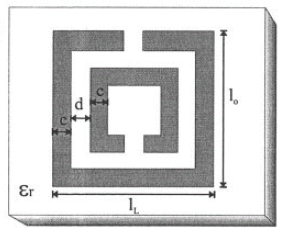
\includegraphics[width=0.4\textwidth]{./images/NotchFilter/squareRingResonator.png} \label{fig:squareResonator}}
 \subfloat[Circular Resonator]{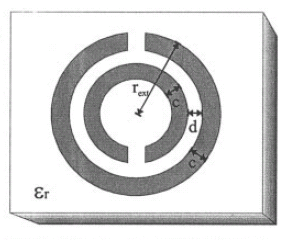
\includegraphics[width=0.4\textwidth]{./images/NotchFilter/circularRingResonator.png} \label{fig:circleResonator}}\\
 \subfloat[Manufactured Bandstop filter with a series of differently tuned square resonator structures]{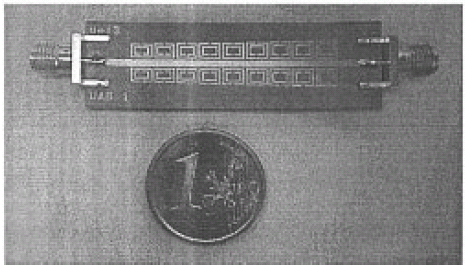
\includegraphics[width=0.4\textwidth]{./images/NotchFilter/Design1.png} \label{fig:design1} } 
\subfloat[S21 Bandstop filter Result- See SRR plot]{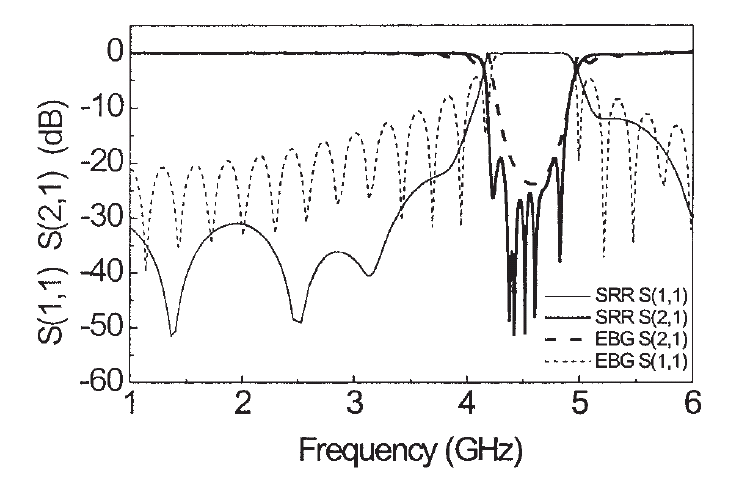
\includegraphics[width=0.4\textwidth]{./images/NotchFilter/s21.png} \label{fig:s21design1} } 
 \caption{Possible resonance structures for the notch filter \cite{Garcia2005}. These diagrams show the dimensions that can be adjusted. We chose to pursue the square type resonance structure \ref{fig:squareResonator}}
 % squareRingResonator.png: 287x238 pixel, 72dpi, 10.12x8.40 cm, bb=0 0 287 238
 \label{fig:squareRingResonator}
\end{figure}

We used these resonators to design 3 initial filters for 4.65~GHz, 4.70~GHz and 4.75~GHz. This we felt would allow use to check that the filter behaved as the simulations predicted across a small range of frequencies.
\clearpage
\subsection{Manufacture and Testing}

\begin{figure}
 \centering
 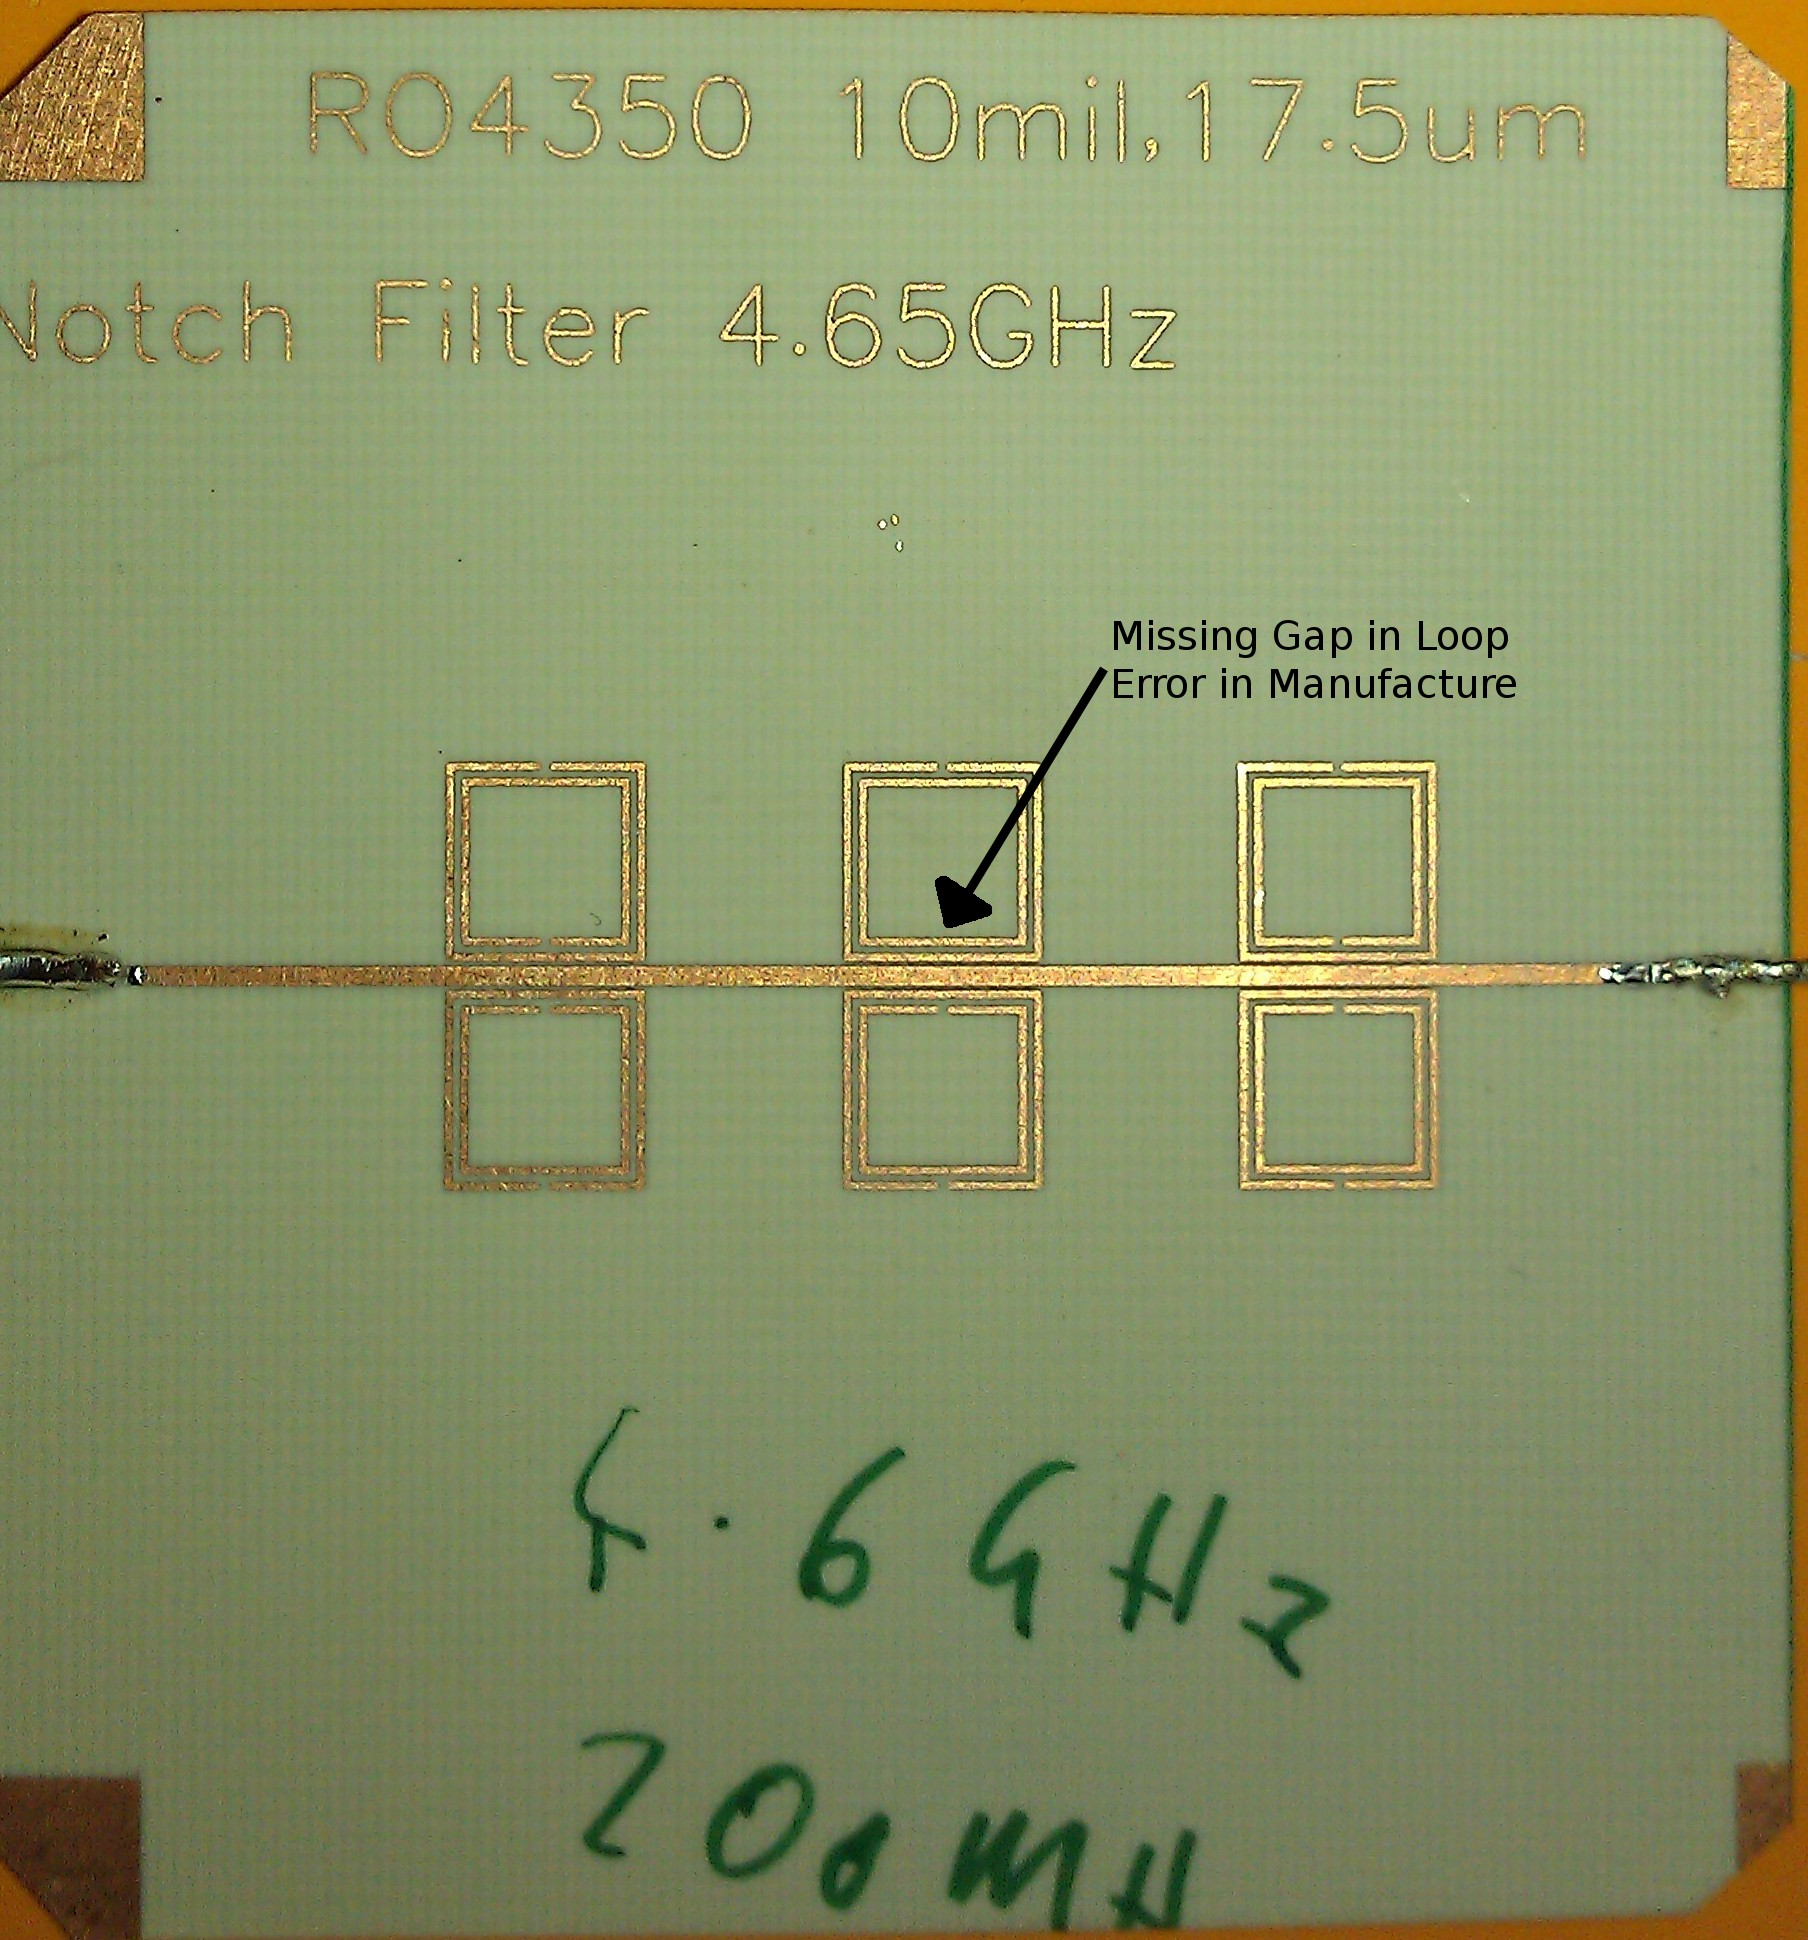
\includegraphics[width=0.5\textwidth]{./images/NotchFilter/IMAG0148.jpg}
 % IMAG0148.jpg: 1808x1940 pixel, 72dpi, 63.78x68.44 cm, bb=0 0 1808 1940
 \caption{The manufactured 4.65~GHz notch filter. Used Rogers RO4350 10mil (Er=3.66) with 17.5um Copper layers for manufacture. Note the error in manufacture. This produced an additional notch feature (apparent in Figure~\ref{fig:MeasuredResults}) at ~10\% higher frequency than the central notch feature. This has been corrected}
 \label{fig:4_65GHzFilter}
\end{figure}


\begin{figure}
 \centering
 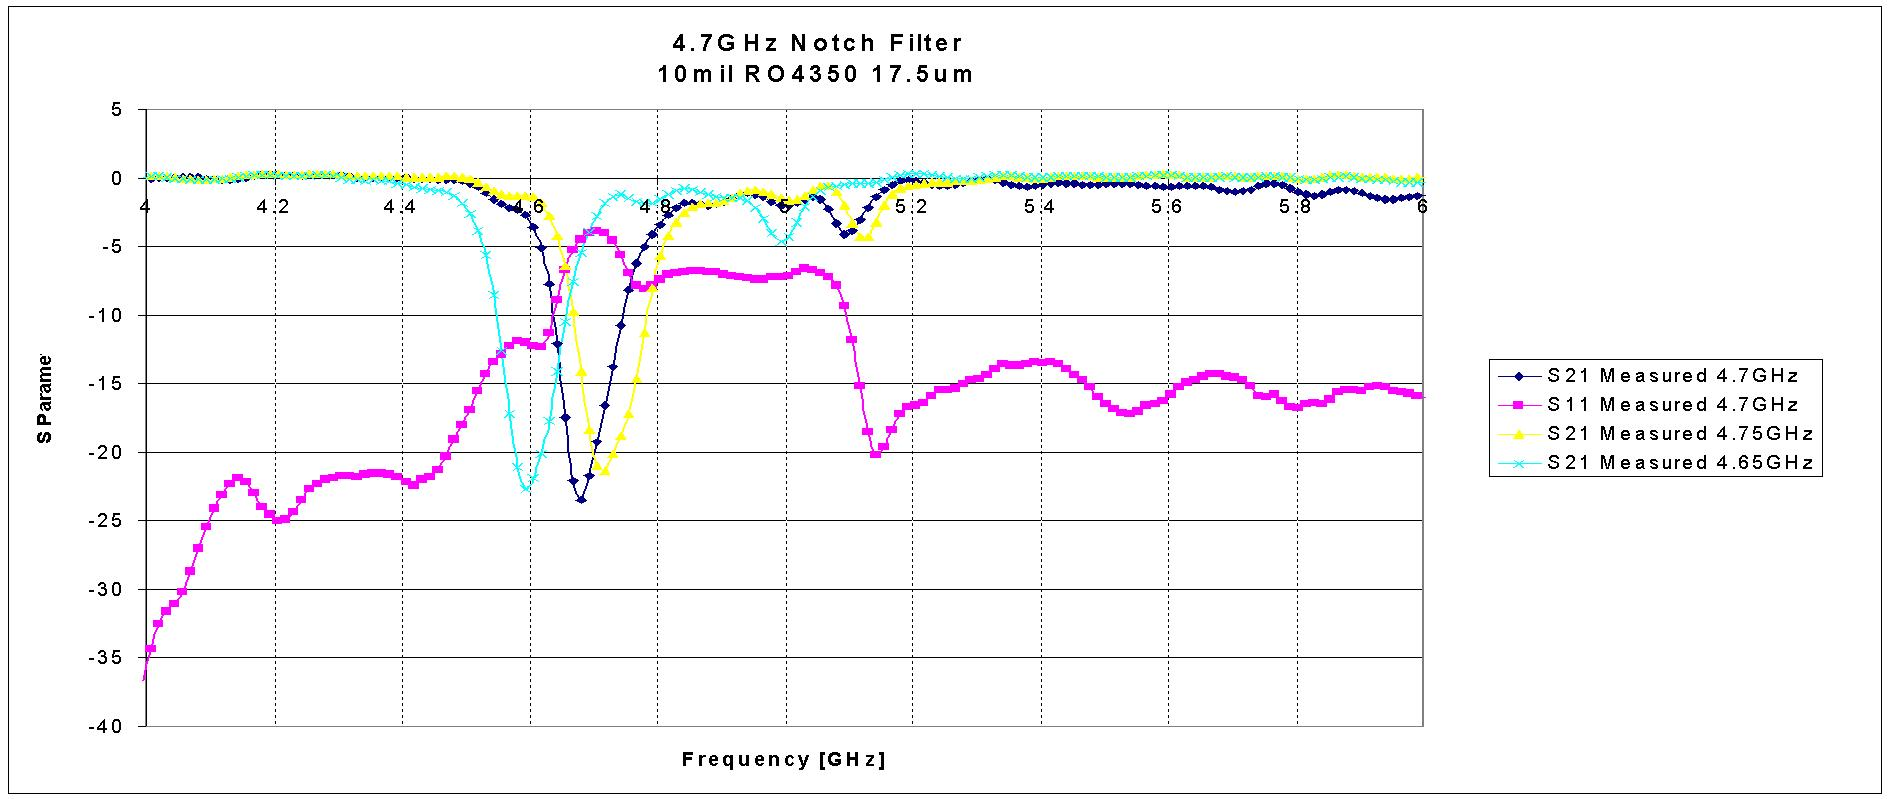
\includegraphics[width=\textwidth]{./images/NotchFilter/MeauredResults.JPG}
 % MeauredResults.JPG: 1890x799 pixel, 96dpi, 50.01x21.14 cm, bb=0 0 1418 599
 \caption{Measured Results of the three square ring resonator structures. We see the additional feature ~10\% higher in frequency caused by the error in manufacture (see Figure~\ref{fig:4_65GHzFilter}) in all three of the designs. We also see that the central notch behaves as we expect although they are approximately 50~MHz lower than the simulations predict}
 \label{fig:MeasuredResults}
\end{figure}

\clearpage
\subsection{Cooling the Filters}

We expected the filter bandwidth to improve at lower temperatures, since most of the loss was resistive loss in the Copper. To test this we initially cooled the design with liquid nitrogen, however we found that the liquid nitrogen effected the central response by changing the dielectric constant of the region directly above the resonator structures.

We decided then to conduct the test in the Oxford test cryostat and achieved the following results.

\begin{figure}[ht]
 \centering
 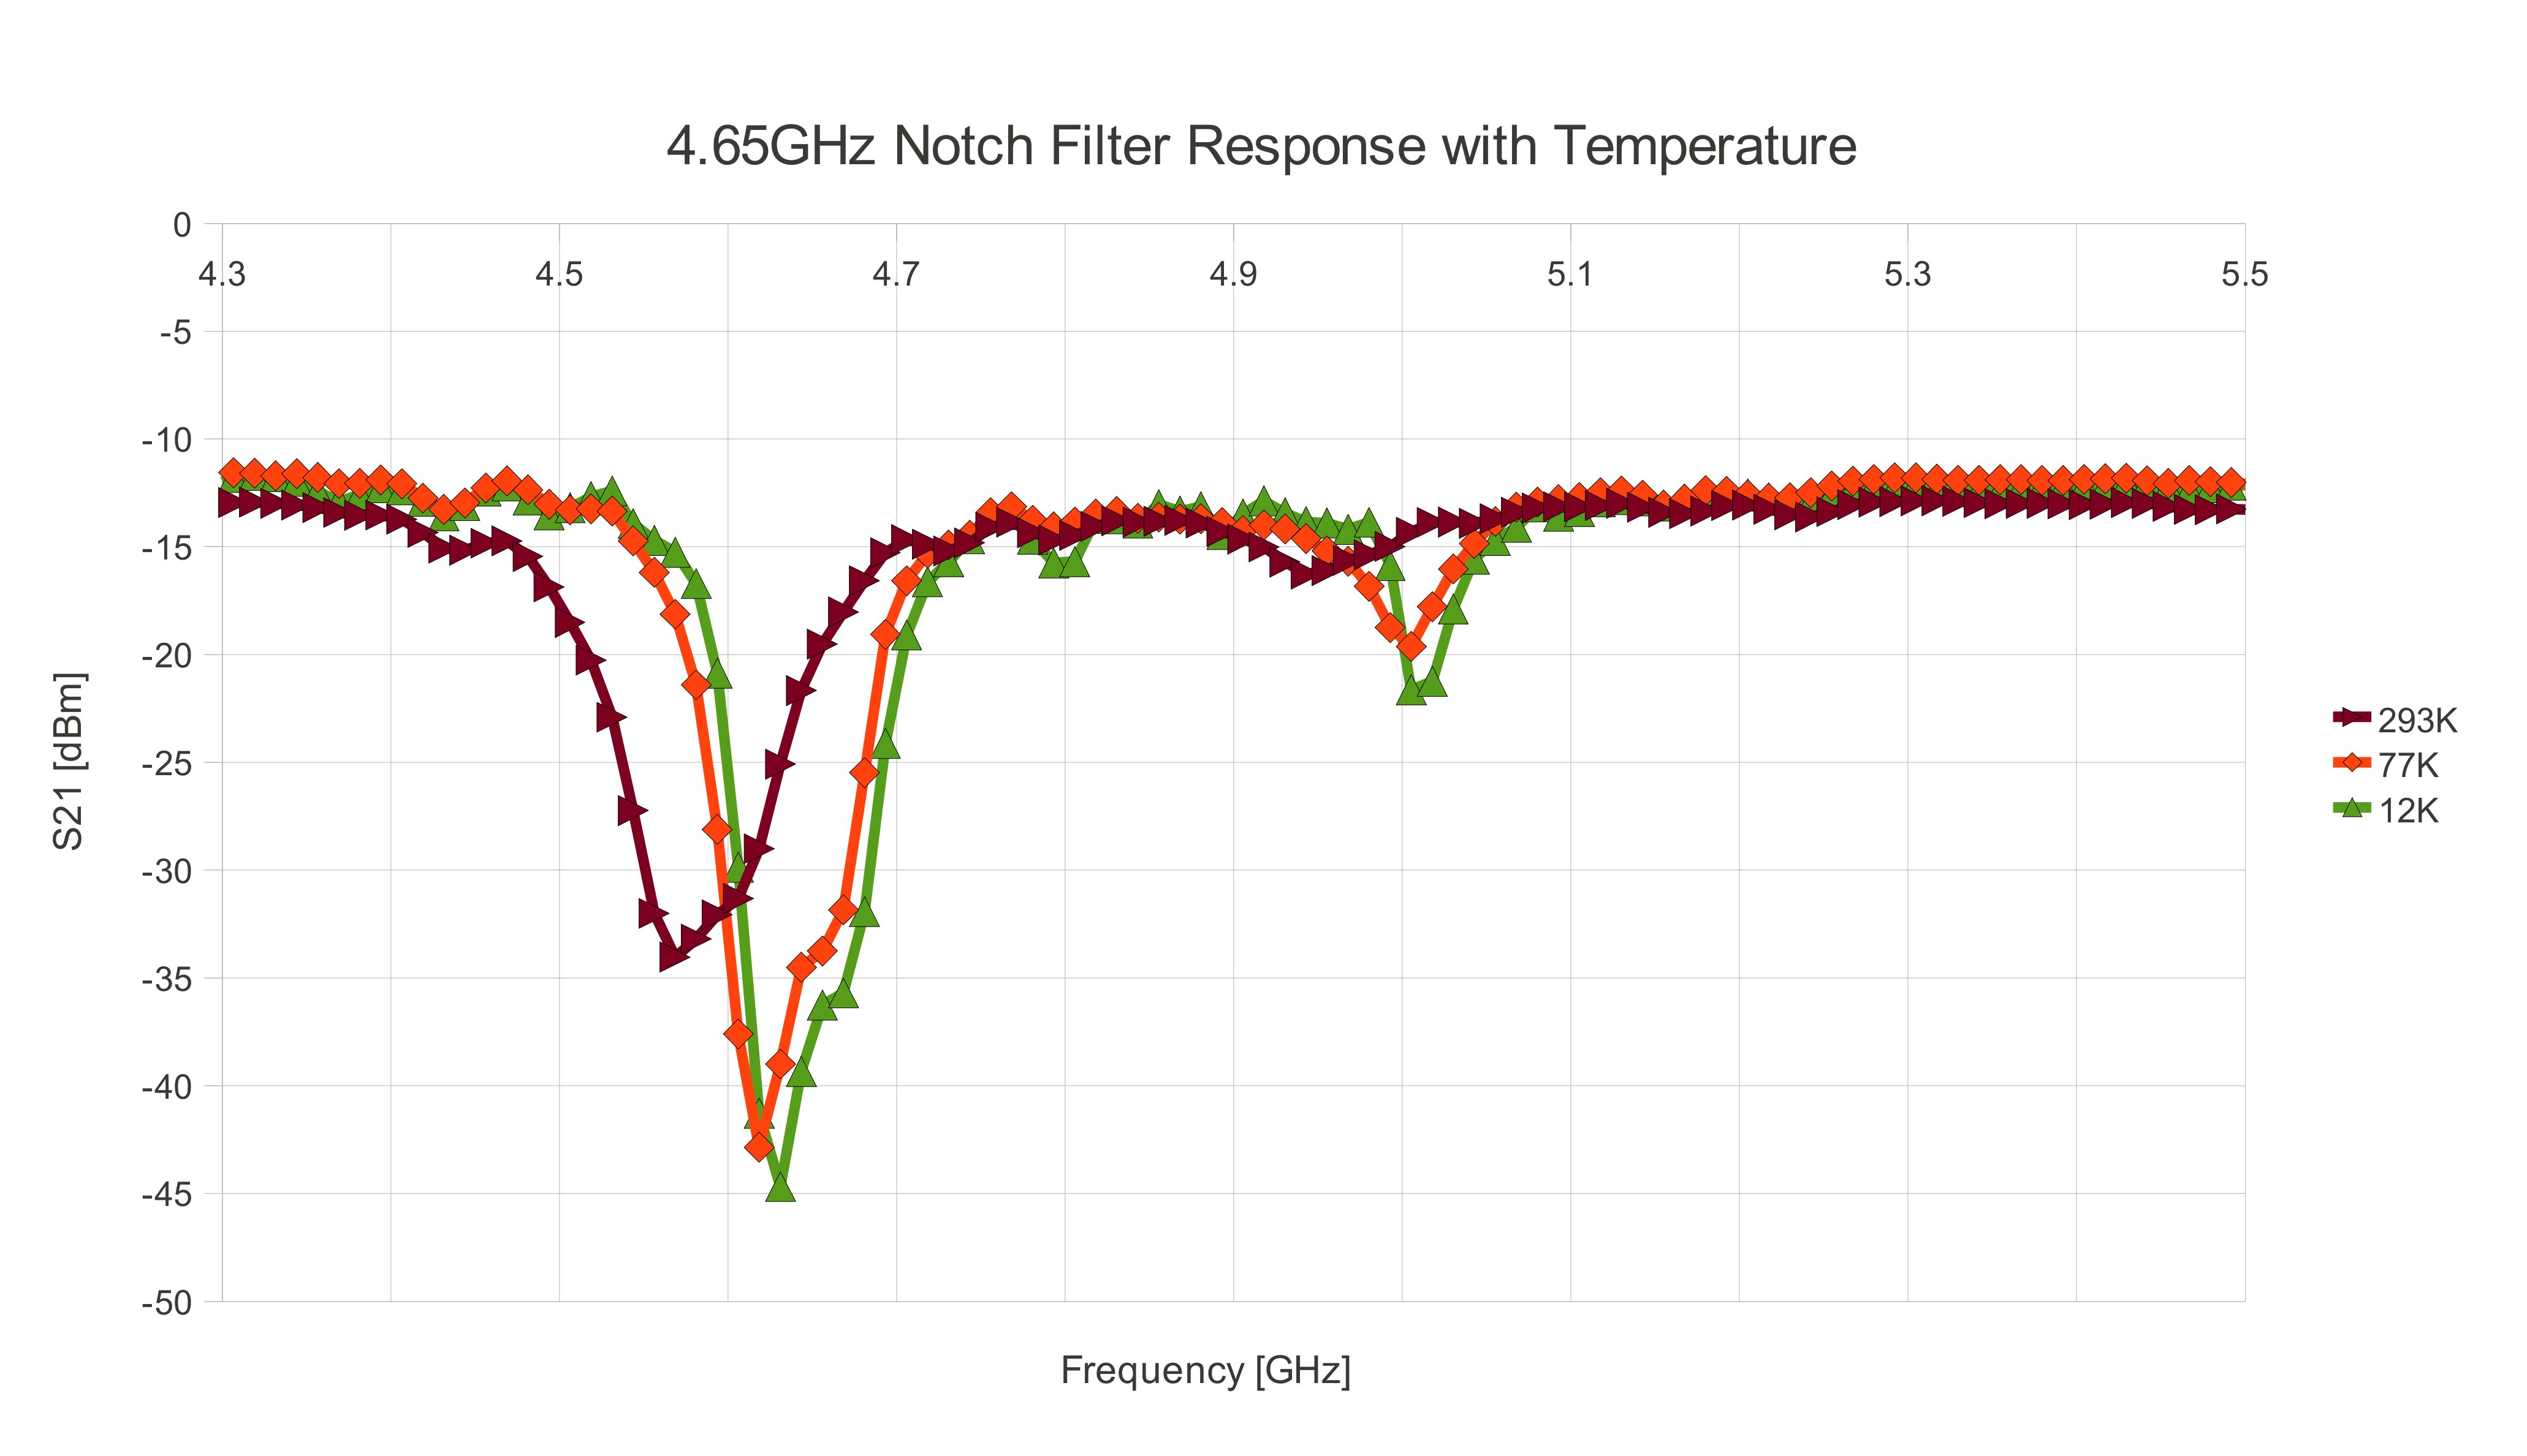
\includegraphics[width=\textwidth]{./images/NotchFilter/CoolingResponse.jpg}
 % CoolingResponse.pdf: 595x842 pixel, 72dpi, 20.99x29.70 cm, bb=0 0 595 842
 \caption{Cooling the Filter in the test cryostat. Note the additional notch feature becomes more pronounce when cooled.}
 \label{fig:coolingResponse}
\end{figure}
\clearpage

\subsection{Filter Installation at Owens Valley Antenna}

The RFI notch filters were installed at the Owens Valley antenna on the 7~May~2011 (see \fign{fig:cryostatInstall}). The filters have successfully suppressed the RFI shown in \fign{fig:RFImaxHold}. The transmission through the cryostat can be seen in \fign{fig:cryostatTransmission}.

\begin{figure}
 \centering
 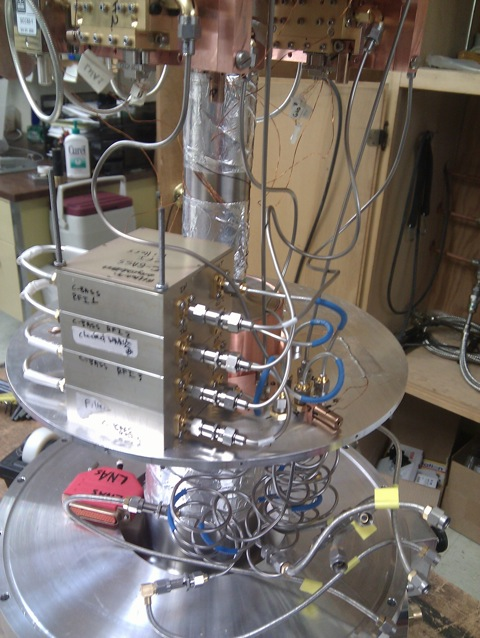
\includegraphics[height=0.6\textheight]{./images/NotchFilter/cryostatInstall.jpg}
 % cryostatInstall.jpg: 480x638 pixel, 72dpi, 16.93x22.51 cm, bb=0 0 480 638
 \caption{The notch filters installed in the cryostat at Owens Valley}
 \label{fig:cryostatInstall}
\end{figure}

\begin{figure}
 \centering
 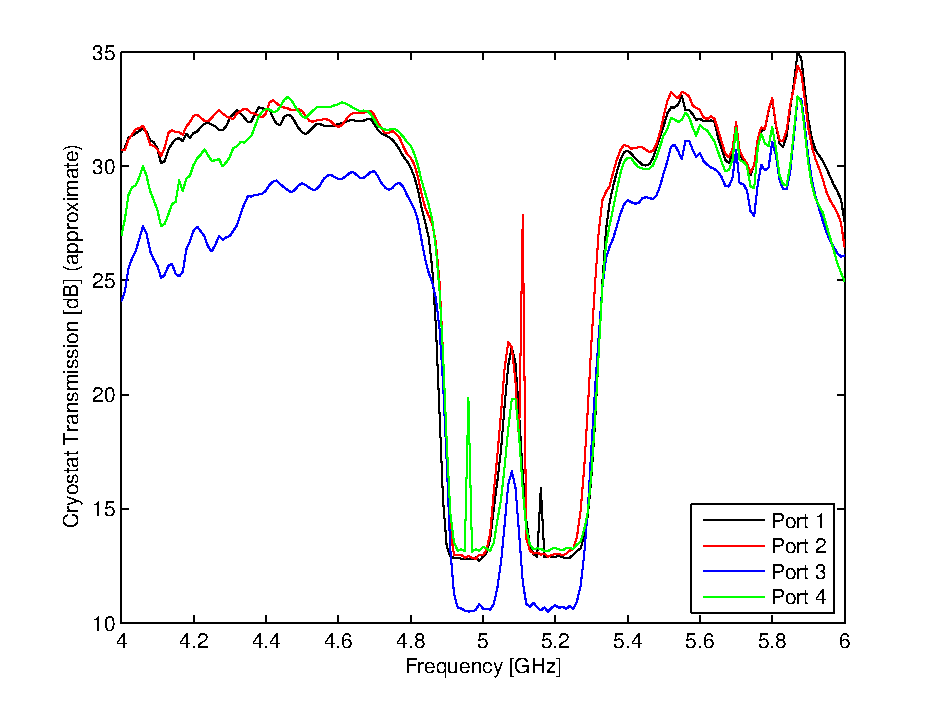
\includegraphics[width=0.6\textwidth]{./images/NotchFilter/CryostatTransmission.pdf}
 % cryostatInstall.jpg: 480x638 pixel, 72dpi, 16.93x22.51 cm, bb=0 0 480 638
 \caption{Transmission through the cryostat after the installation of the notch filters. The two stop bands prevent incoming RFI from contaminating the signal}
 \label{fig:cryostatTransmission}
\end{figure}
% 

\subsection{Other Possibilities}

High temperature superconducting filters \cite{Futatsumori2008}, would achieve much higher Q values, allowing us to design filters for each of the RFI features. However the manufacture process is complicated, and in addition would be a new method for the Physics department. In addition, the frequency distribution of the four RFI signals obviate any significant advantage of higher Q filters.

The other possibility is to switch over to a digital polarimeter, a clone of the new Southern receiver.  \clearpage
\chapter{The Southern Receiver and Component Designs}

\section{Motivation}

  \subsection{Block Diagram}

\begin{figure}[ht]
 \centering
 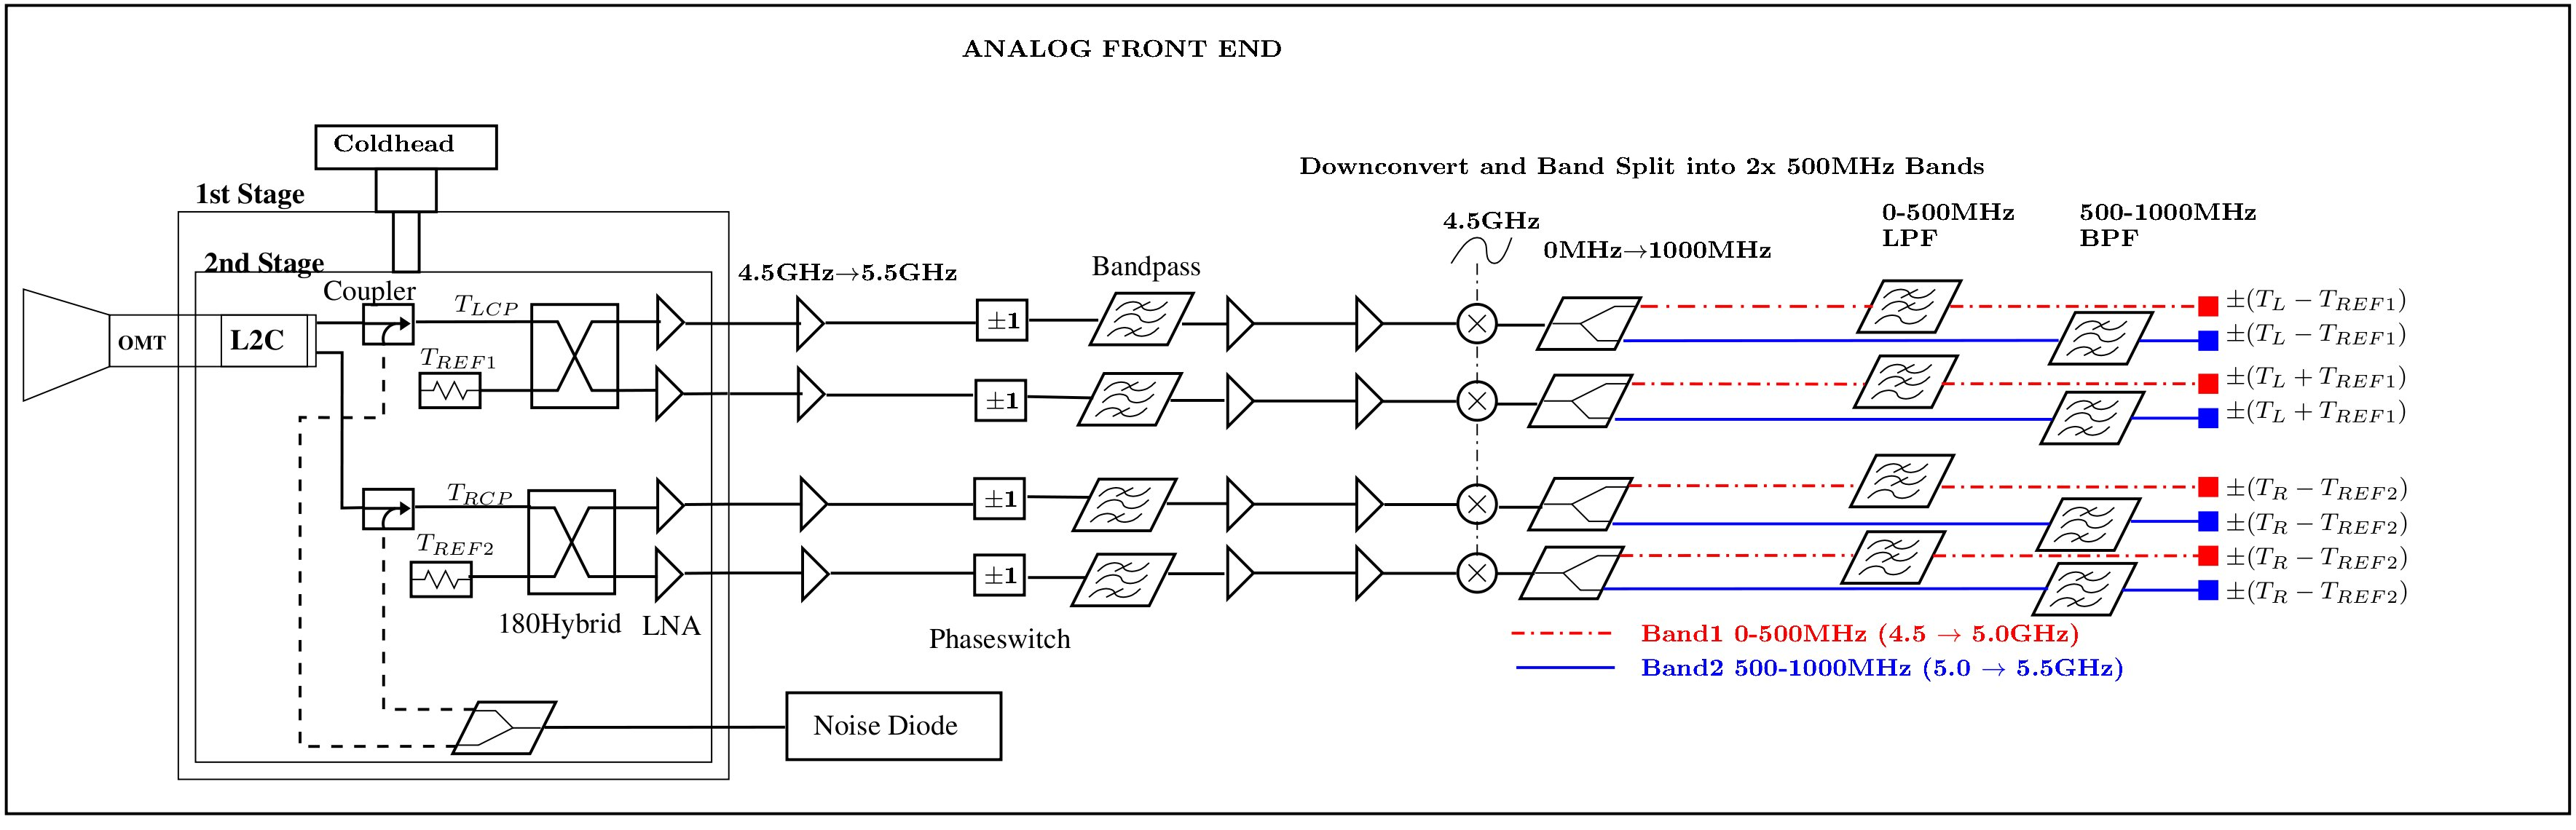
\includegraphics[width=\textwidth,height=0.4\textheight]{images/receiver_schematics/rfNew.jpg} % analog.png: 1920x1200 pixel, 72dpi, 67.73x42.33 cm, bb=
 \caption{Diagram of the analog front end of the digital receiver. There are significantly fewer analog components than the Northern Hemisphere polarimeter (see \appen{sec:pseudoCorrelation}, \fign{fig:analog_receiver}). The diagram shows the down-conversion of the 1~GHz band (into two 500~MHz bands) followed by the ADC capture. The digital processing is shown on \fign{fig:digital_receiver_mine}  }
 \label{fig:digital_receiver}
\end{figure}

\begin{figure}[ht]
 \centering
 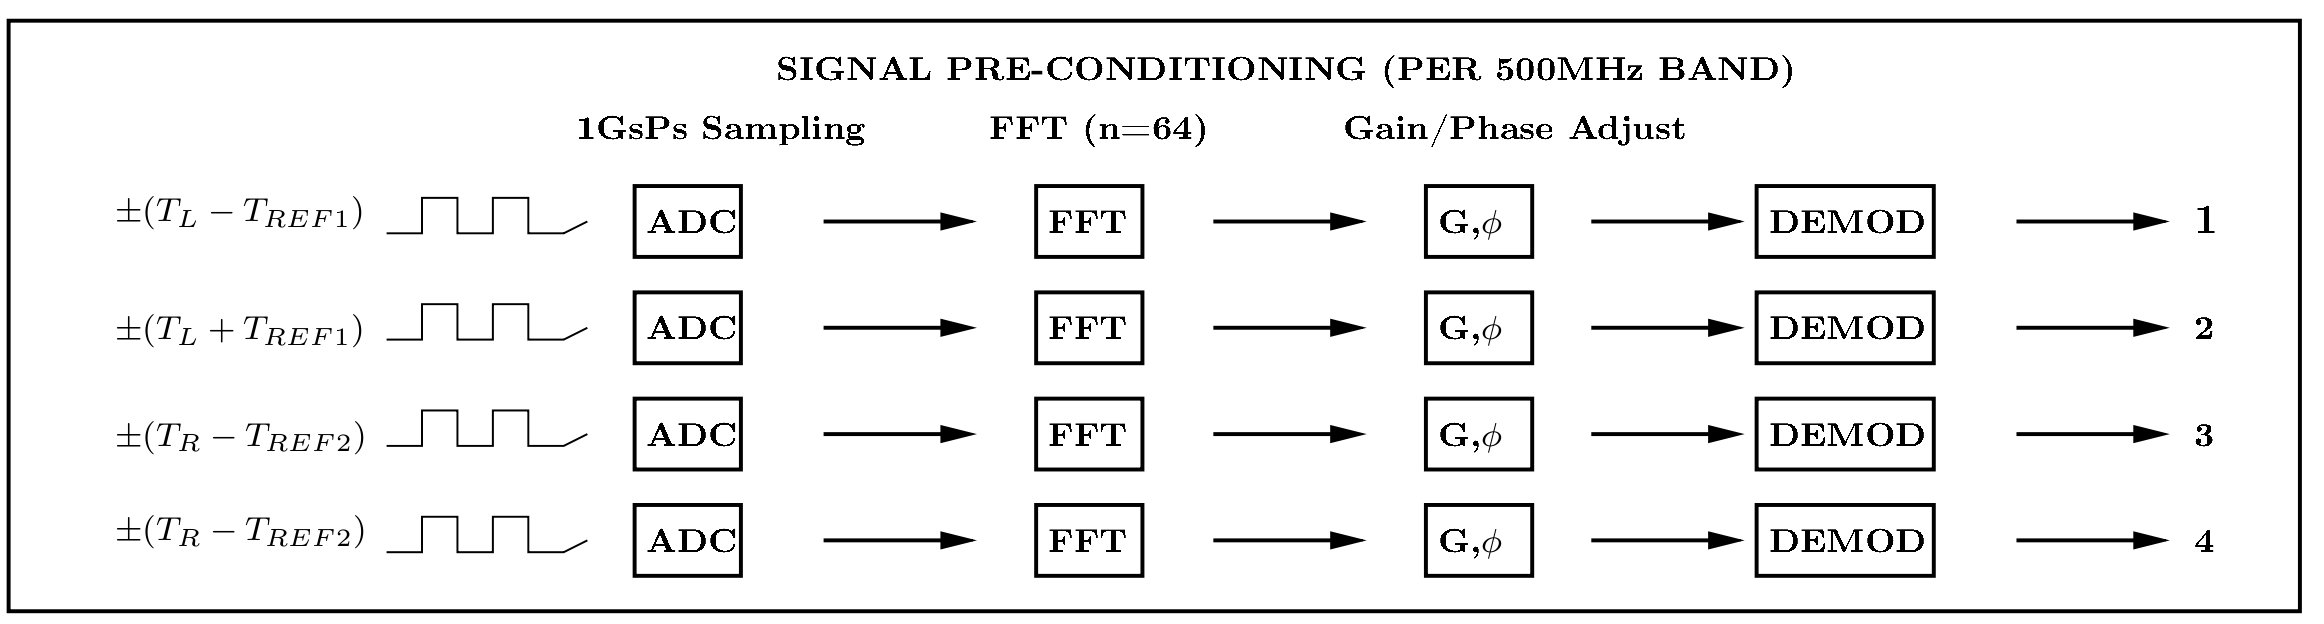
\includegraphics[width=\textwidth]{images/receiver_schematics/precon.jpg}\\
 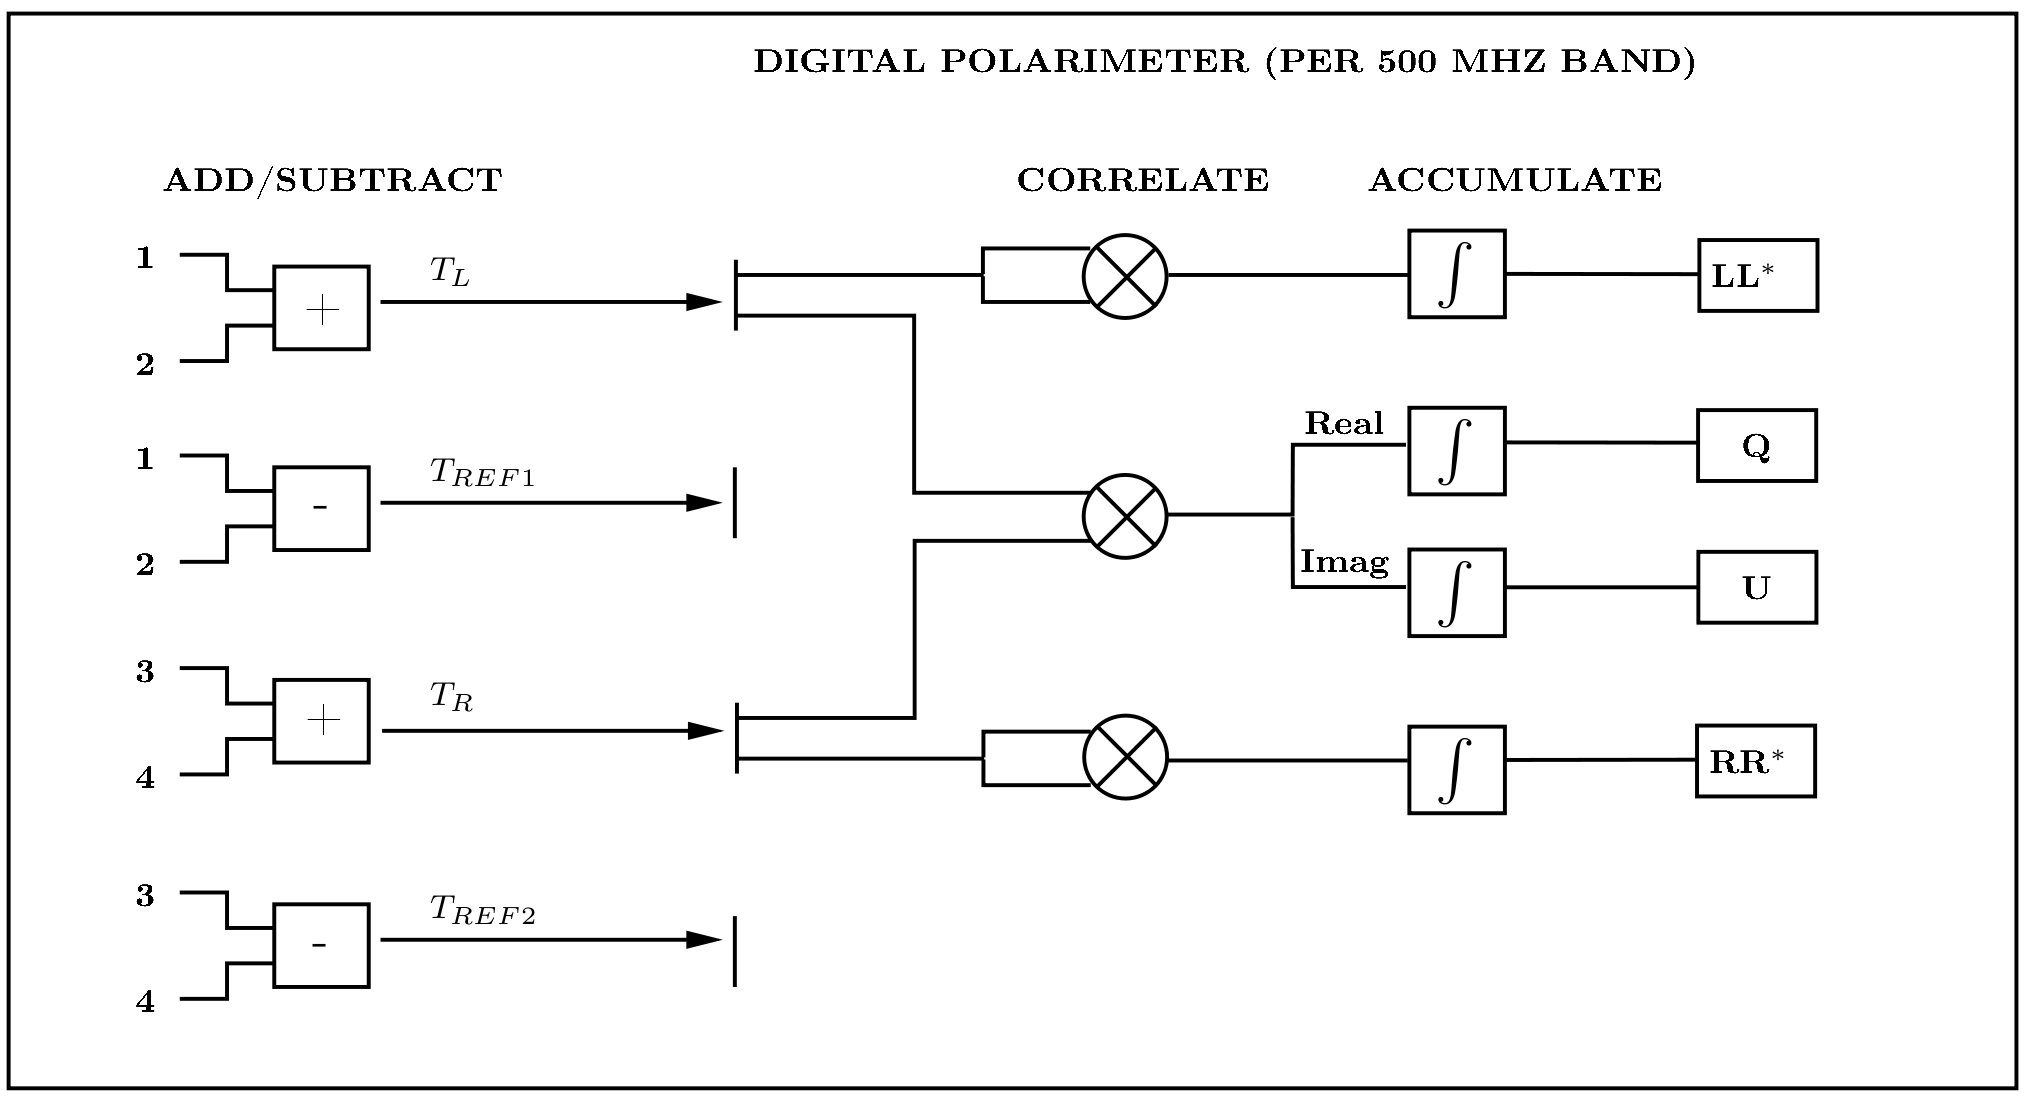
\includegraphics[width=\textwidth]{images/receiver_schematics/roach.jpg}
 % analog.png: 1920x1200 pixel, 72dpi, 67.73x42.33 cm, bb=
 \caption{Diagram of the digital polarimeter. The diagram shows one of the 500~MHz bands. The signals are sampled, fast-Fourier transformed, gain and phase adjusted, demodulated, added, correlated and then accumulated to produce the values required for the Stokes parameters. See \appen{sec:stokes}, Equations~\ref{eq:stokes_circ_I}$\rightarrow$\ref{eq:stokes_circ_V} for clarification on the correlations used to produce the Stokes parameters}
 \label{fig:digital_receiver_mine}
\end{figure}
\clearpage


  \subsection{Designs Choices}


\subsection{Passive Component Insertion Loss}

The system temperature of a radio receiver is given by the \eqn{eq:Friis_Equation}: the Friis Equation.

\begin{equation}
 T_{sys} = T_{sky}+T_{spillover}+T_{optics} + \frac{T_{horn}}{G_{optics}} + \frac{T_{passives}}{G_{optics}G_{horn}}+\frac{T_{LNA}}{G_{optics}G_{horn}G_{passives}}
\label{eq:Friis_Equation}
\end{equation}

The continuous-comparison scheme used in the C-BASS receiver is complicated. The receiver requires significant pre-LNA passive components all of which are lossy. 

From \eqn{eq:Friis_Equation} we see that any pre-LNA loss needs to be avoided. It hurts the system, not just in terms of the individual component resistive noise contribution $(1-L)T_{phys}$, but also in terms of the effect these losses have on subsequent components, in particular the LNA noise contribution, where a 3~dB passive loss will increase the effective noise contribution of the LNA by a factor of 2. 

RF loss takes one of three forms: resistive losses, mismatch losses, dielectric losses. 

Resistive losses hurt the system temperature both by introducing additional noise (proportional to the temperature of the resistor) as well as reducing the signal noise. In a cryogenic radio receiver, losses before the cryostat (warm losses) occur at ~300~K while losses inside the cryostat (cold losses) are at the cryogenic operating temperature (for C-BASS South this is 10~K). We can easily see that the 'warm losses' are best avoided. 

Mismatch losses occur where there is a slight discontinuity in the impedance of the RF path. Classic examples are RF connectors and RF launches onto substrate. Impedance mismatches, cause reflection of the signal, reducing the signal power. These losses do not result in additional noise themselves, but increase the effective noise figure of the amplifier later in the chain.

Dielectric losses occur due to dissipation of electromagnetic energy in the dielectric (effectively heating the dielectric). The losses are proportional to the frequency of the RF.



In the C-BASS architecture, passive loss is difficult to avoid. Consider for a moment the coaxial interconnects between components. One could be forgiven for assuming that the majority of the cable loss resistive, and thus that cooling a coaxial cable assembly (and thus reducing the resistances) will reduce the total cable assembly insertion loss. However this completely ignores the dielectric loss of a coaxial cable and the mismatch loss of the mated connectors. These are not neglible, and need to be understood.

\subsubsection{Coaxial Cable Insertion Loss Model}

\citeasnoun{Pozar2005} models the various we expect in a typical coaxial tranmission line. Here $D$ is the diameter of the outer conductor, and $d$ is the diameter of the inner conductor.

\begin{equation}
 Resistance/length=\left ( \frac{f\mu_{0}}{\pi} \right ) ^{\frac{1}{2}}  \left ( \frac{(\mu_{R1}\rho_{1})^{\frac{1}{2}}}{D} + \frac{(\mu_{R2}\rho_{2})^{\frac{1}{2}}}{d}\right ) 
\label{eq:resistance_length}
\end{equation}

\begin{equation}
 Z_{0}=\frac{138}{\sqrt{\epsilon_{R}}}log \left (\frac{D}{d} \right )
\label{eq:impedance}
\end{equation}

Loss in a coaxial assembly is given by $Loss=Resistance/2Z_{0}$, so combining \eqn{eq:resistance_length} and \eqn{eq:impedance} we arrive at
\begin{eqnarray}
 Loss/length&=&\frac{1}{138 \times 2}\left ( \frac{\epsilon_{R}f\mu_{0}}{\pi} \right ) ^{\frac{1}{2}}  \left ( \frac{(\mu_{R1}\rho_{1})^{\frac{1}{2}}}{D} + \frac{(\mu_{R2}\rho_{2})^{\frac{1}{2}}}{d}\right ) \frac{1}{log\left ( \frac{D}{d} \right )} Np/m\\
\end{eqnarray}

Insertion loss due to dielectric loss of a TEM wave propagating through a coaxial cable as

\begin{equation}
 \alpha_{d}=\frac{\pi \epsilon_{r} tan \delta}{\lambda} Np/m
\label{eq:dielectric_attenuation}
\end{equation}

Another, often omitted loss of a cable assembly, is the connector loss. A typical mated SMA connector has $0.03\sqrt{f_{GHZ}}$~dB ossMeasuring the passive componetns in the cryostat requires careful thought. The ~24hour turnaround between measurements is time intensive and careful consideration needs to be taken to optimise measurments.

The test cable assembly requires initial characterisation. 


\clearpage

\section{Digital Hardware}
\subsection{Roach}

\subsection{iADC}
The iADC is a multi-purpose CASPER analog-to-digital convertor based around the Atmel/e2V AT84AD001B IC. In non-interleaved mode the ADC is capable of sampling 4 signals as 1GsPs i.e a 500~MHz bandwidth. 

\subsubsection{Power Levels}
Tests were carried out to monitor the linearity of the Casper iADC 4-Chann

\subsubsection{Linearity}
\subsubsection{Van Fleck Corrections}

\section{Low Frequency Filters}
AS has been explained, the C-BASS is designed for the 4.5$\rightarrow$5.5~GHz band. This band is defined using edge-coupled filters early in the RF chain. After suitable RF amplification, the signal is downcoverted using a 4.5~GHz LO, mapping 4.5GHz->DC and 5.5GHz to 1~GHz.
In the digital C-BASS we chose to split this 1~GHz band. One iADC/ROACH would sample the first Nyquist Zone (DC-500MHz) and another would sample the second Nyquist Zone (500-1000MHz). We chose to rely on the earlier edge-coupled filters to define the DC and 1GHz roll-off, and required a suitable 500~MHz low pass filter and 500~MHz high pass filter. 

The requirements were small form factor, 20dB roll off in the first 20MHz of band overlap and manufacturability.


\subsection{Filter Design}
\label{sec:lowfreqFilters}

For the design shown in \fign{fig:digital_receiver}, two low frequency filters are required: a 500~MHz lowpass filter and a 500$\rightarrow$1000~MHz bandpass filter.

The difficulty of designing filters in the 1GHz frequency range is that it straddles two design regions \cite{matthaei1980} . Generally higher frequency filters are designed using strip line which scale in size with wavelength making them unsuitable for use at low frequencies. Low frequency designs have tended to use lumped-element capacitors and inductors, but these are notoriously difficult to use at higher frequencies where parasitic effects become important.

The design we have employed uses a lumped-element based approach from  with ongoing development and simulations in the \textit{Microwave Office} software suite. Careful use of standardised, well understood, high quality components has allowed us to build filters at unusually high frequencies usually with rapid turnaround times. This makes use of published component values from Murata \cite{murataAWR}

Results so far are very promising. The 0$\rightarrow$500~MHz Low pass filter is complete (see Figure~\ref{fig:LowFrequency0_500MHz}) and we are rapidly converging on a suitable band-pass filter for the 500$\rightarrow$1000MHz band Figure~\ref{fig:LowFrequency500_1000MHza}. Our understanding of the behaviour of the Murata components at high frequencies has improved significantly since this version of the bandpass filter.



\begin{figure}
 \centering
\subfloat[][Lowpass filter design schematic]{
 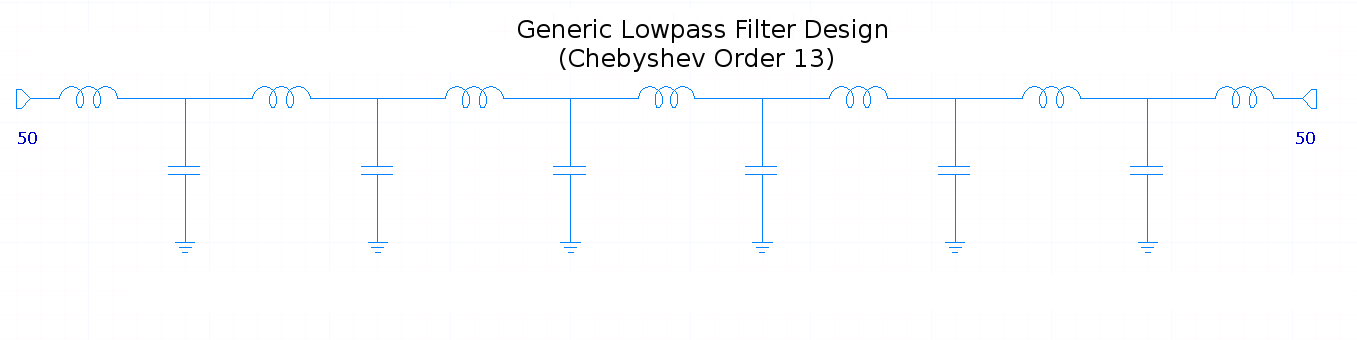
\includegraphics[width=\textwidth]{./images/LowFrequencyFilters/lowpass.png}
}\\
\subfloat[][Bandpass filter design schematic]{
 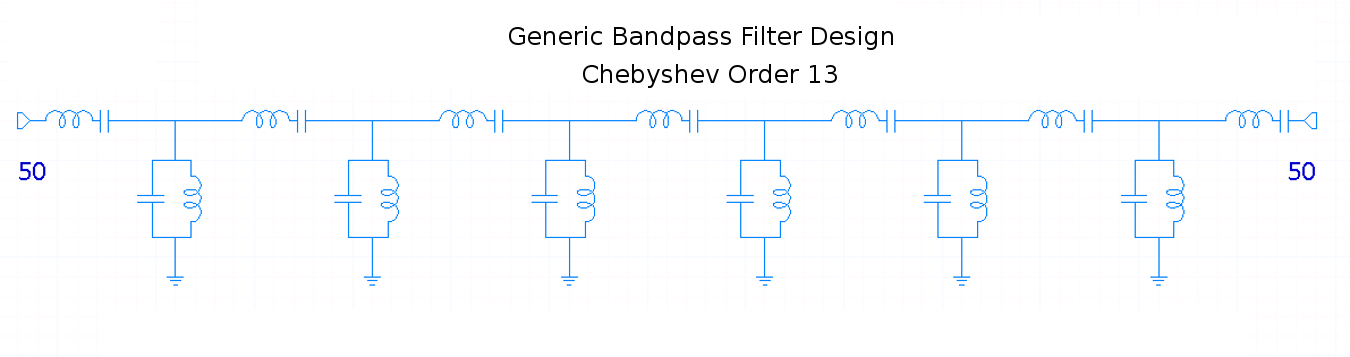
\includegraphics[width=\textwidth]{./images/LowFrequencyFilters/bandpass.png}
}


 % lowpass.png: 1357x340 pixel, 72dpi, 47.87x11.99 cm, bb=0 0 1357 340
 \caption{Low frequency lumped element filter designs and manufacture}
 \label{fig:filterDesigns}
\end{figure}


\begin{figure}
 \centering
\subfloat[][]{
 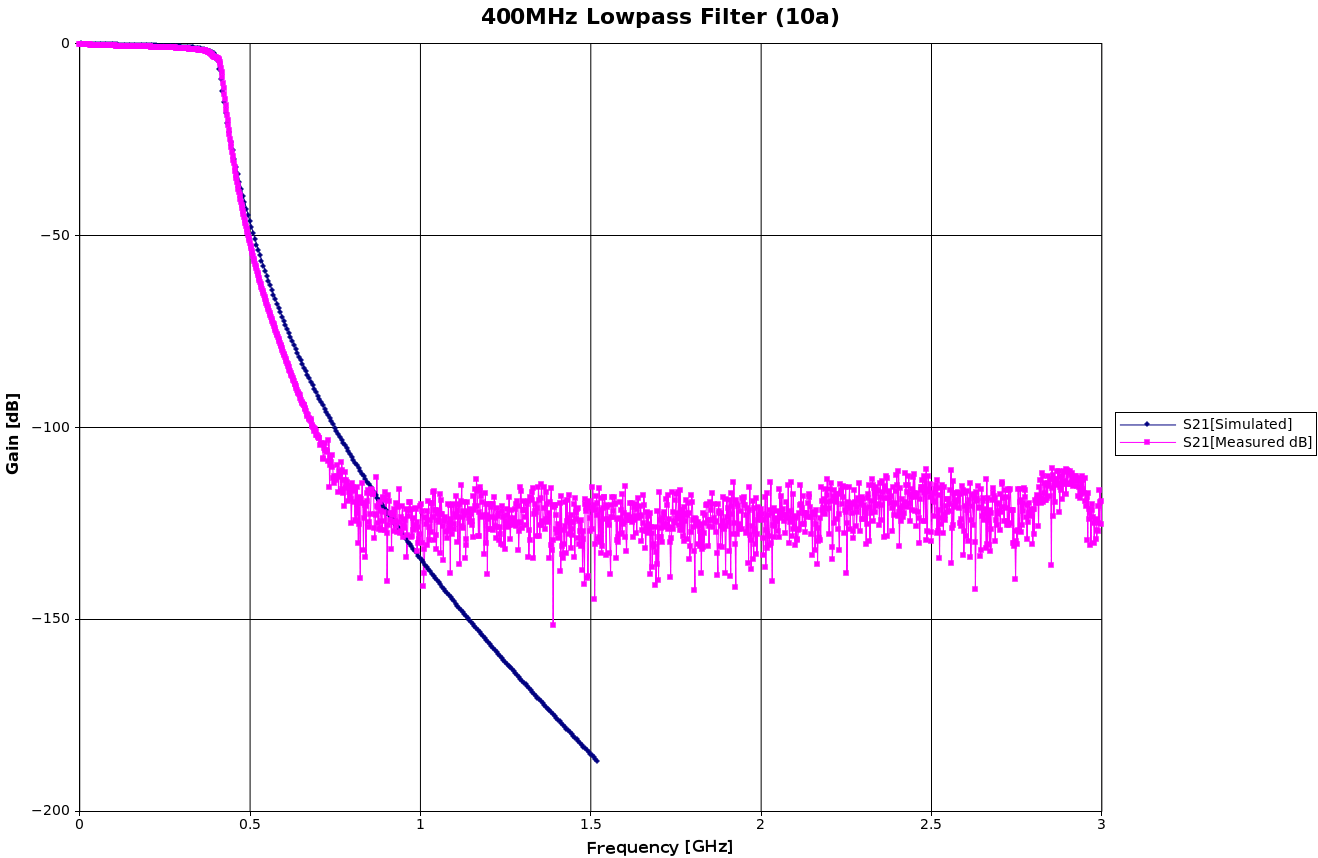
\includegraphics[height=0.4\textheight]{./images/LowFrequencyFilters/lpf10asimvsmeasured1.png}
}\\
\subfloat[][]{
 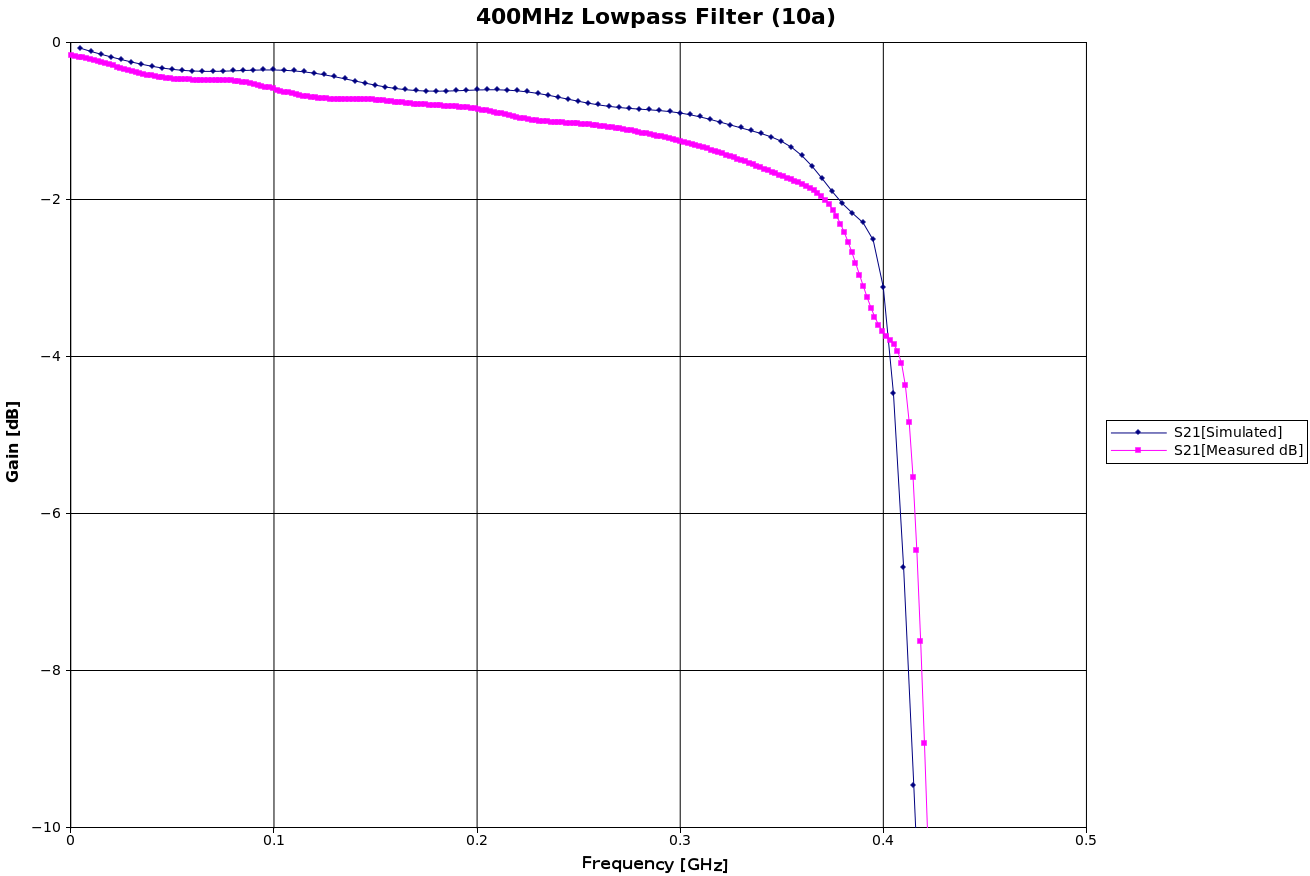
\includegraphics[height=0.4\textheight]{./images/LowFrequencyFilters/lpf10asimvsmeasured2.png}
}
 % lpf10asimvsmeasured1.png: 1571x1046 pixel, 72dpi, 55.41x36.90 cm, bb=0 0 1571 1046
 \caption{Simulated filter performance against measured performance. }
 \label{fig:simvsmeasuredlpf10a}
\end{figure}


We focused on using a design/manufacture technique that would allow rapid prototyping of these filters, and allow quick turnaround times for custom filters that might be required in the future. The techniques we have developed allow a custom filter built in a day, with the major bottleneck still being availability of components. This allows significantly more flexible designs to be produced than was the case previously. In addition, the technique opens up the possibility of building compact filters directly onto printed circuit boards using pick and place for mass production. This has potential for use in large scale radio astronomy deployments such as the Square Kilometer Array. 

% \begin{figure}
%  \centering
%  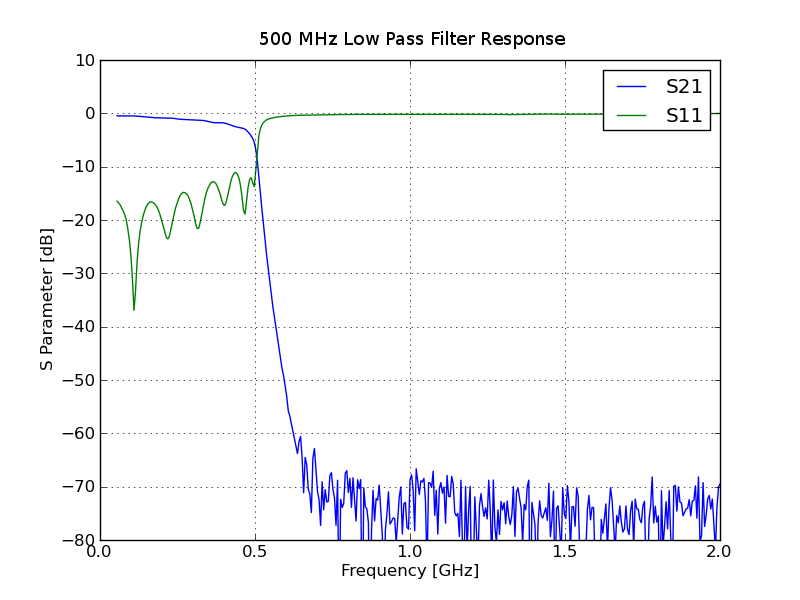
\includegraphics[width=0.5\textwidth]{./images/LowFrequencyFilters/LPF1.png}
%  \caption{The 0$\rightarrow$500MHz Low pass filter. }
%  \label{fig:LowFrequency0_500MHz}
% \end{figure}


 
\begin{figure}
 \centering
\subfloat[The 0$\rightarrow$500MHz Low pass filter.]{
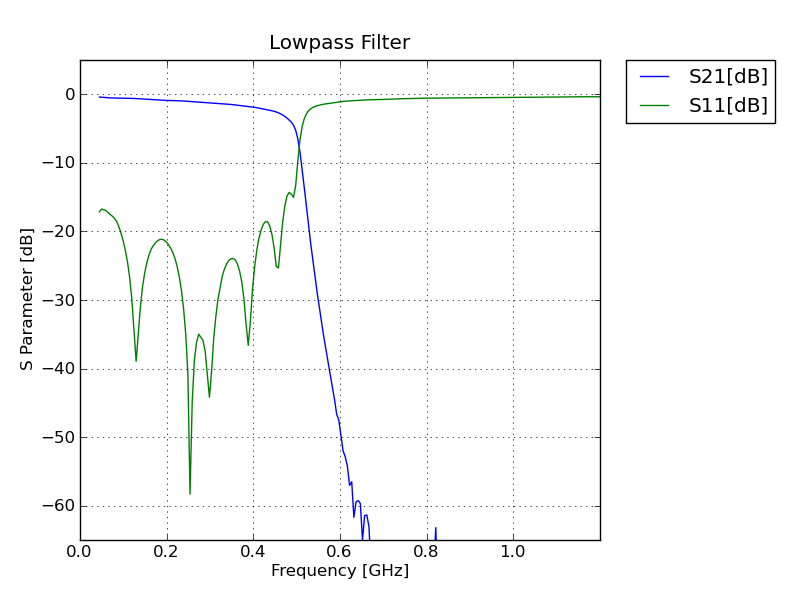
\includegraphics[width=0.5\textwidth]{./images/LowFrequencyFilters/LowpassFilter.png}
\label{fig:LowFrequency0_500MHz}
}\\
\subfloat[The 1000~MHz low pass filter ]{
 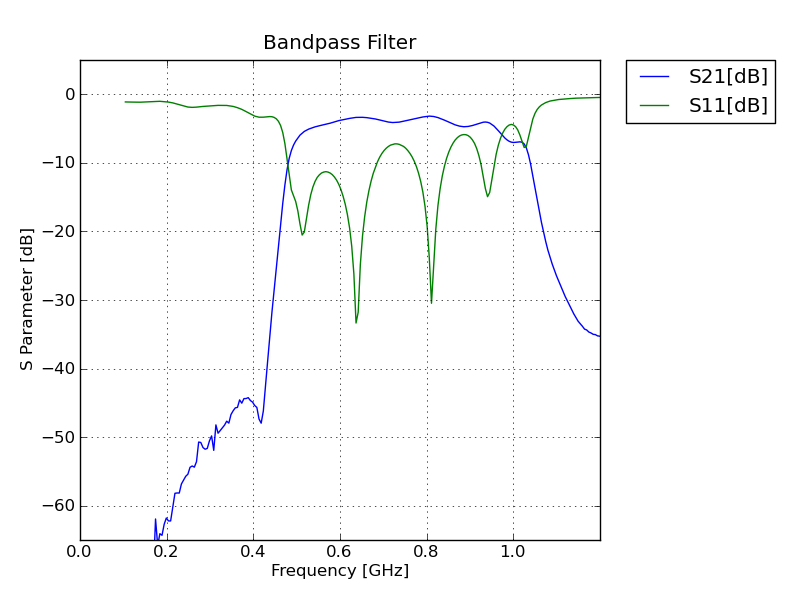
\includegraphics[width=0.5\textwidth]{./images/LowFrequencyFilters/BandpassFilter}
\label{fig:LowFrequency500_1000MHza}}
\label{fig:LowFrequencyFilters} 
\caption{The 500~MHz lowpass filter and the 500$\rightarrow$1000MHz bandpass filter. Since the bandpass filter operates at high frequenciess where lumped element design is difficult, we decided to make the band pass filter from a cascaded high pass filter (500MHz) and low pass filter (1000MHz). This allowed us to optimise the high end and low end independently. There is still a little work to do on the 1000~MHz filter (i.e the high end of the bandpass filter), but out understanding of these components' behavious at high frequency has improved significantly, and we believe this will be reflected in the next iteration}
\end{figure}


 \subsection{Component Choices}
At low frequencies filters are usually designed using surface mount or axial components. At low frequencies parasitic effects are negligible, however at higher frequencies the parasitic inductances and capacitances of the components need to be carefully considered during design. 

Many manufacturers release component libraries, which quantify these parasitics as well as other parameter changes with frequency. We chose to use Murata components, because of availability of suitable components in low quantities. 

Surface mount inductors can present significant challenges at high frequencies. Parasitic capacitance exists due to electric fields between small potential differences between the wire coils, and the wire itself presents a parasitic resistance. We tried the LQW18/LQW15 wire wound type inductors and the LQG18/LQG15 multilayer inductors \cite{murataInductors}. The manufacturing style of both is shown in \fign{fig:inductorStyles}. Both provide ranges from 1nH$\rightarrow$270nH and are designed for use at high frequencies.

\begin{figure}[ht]
 \centering
 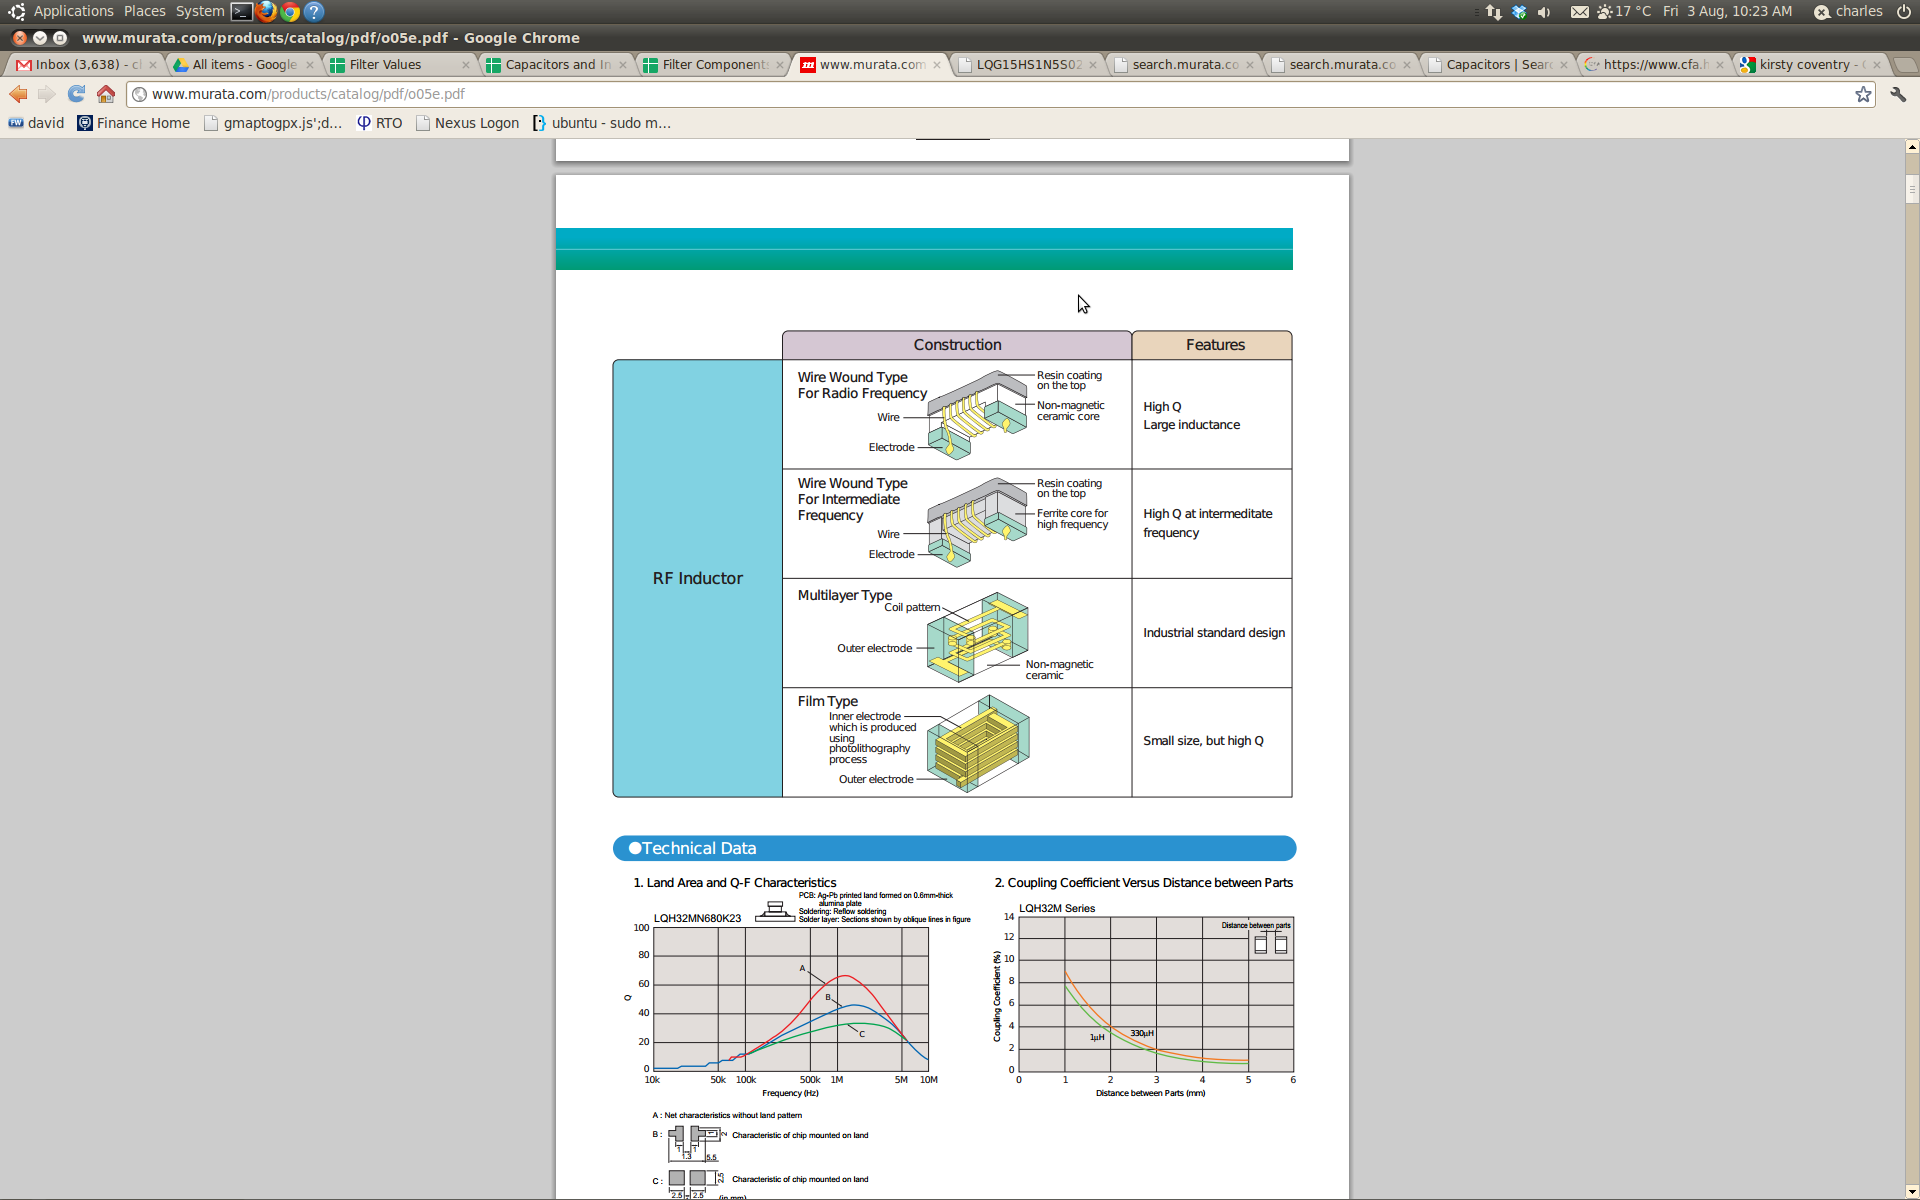
\includegraphics[width=\textwidth]{./images/LowFrequencyFilters/inductorStyles.png}
 % inductorStyles.png: 1920x1200 pixel, 72dpi, 67.73x42.33 cm, bb=0 0 1920 1200
 \caption{Different manufacturing styles of chip inductors \cite{murataInductors}}
 \label{fig:inductorStyles}
\end{figure}

For capacitors we chose the GJM15 Series ceramic capacitors also from Murata \cite{MurataCapacitors}. These are specifically designed for high frequency operations (up to 10~GHz), and are readily available across the full range of values from 0.1pF$\rightarrow$33pF. They feature low ESR (parasitic series resistance) (see \cite{MurataCapacitors} for values) 


  \subsection{Manufacture Techniques and Packaging}

Component choice is an important consideration, as is symmetry in the design. We have used coplanar waveguide to allow access to the ground plane on the top side of the board, and have laid out the components in a symmetrical fashion. As can be seen in \fign{fig:filterBoxing}, careful consideration also needs to be given to the way in which the filter boards are packaged. The packaging plays an important role in improving the out of band rejection characteristics.

\begin{figure}
 \centering
 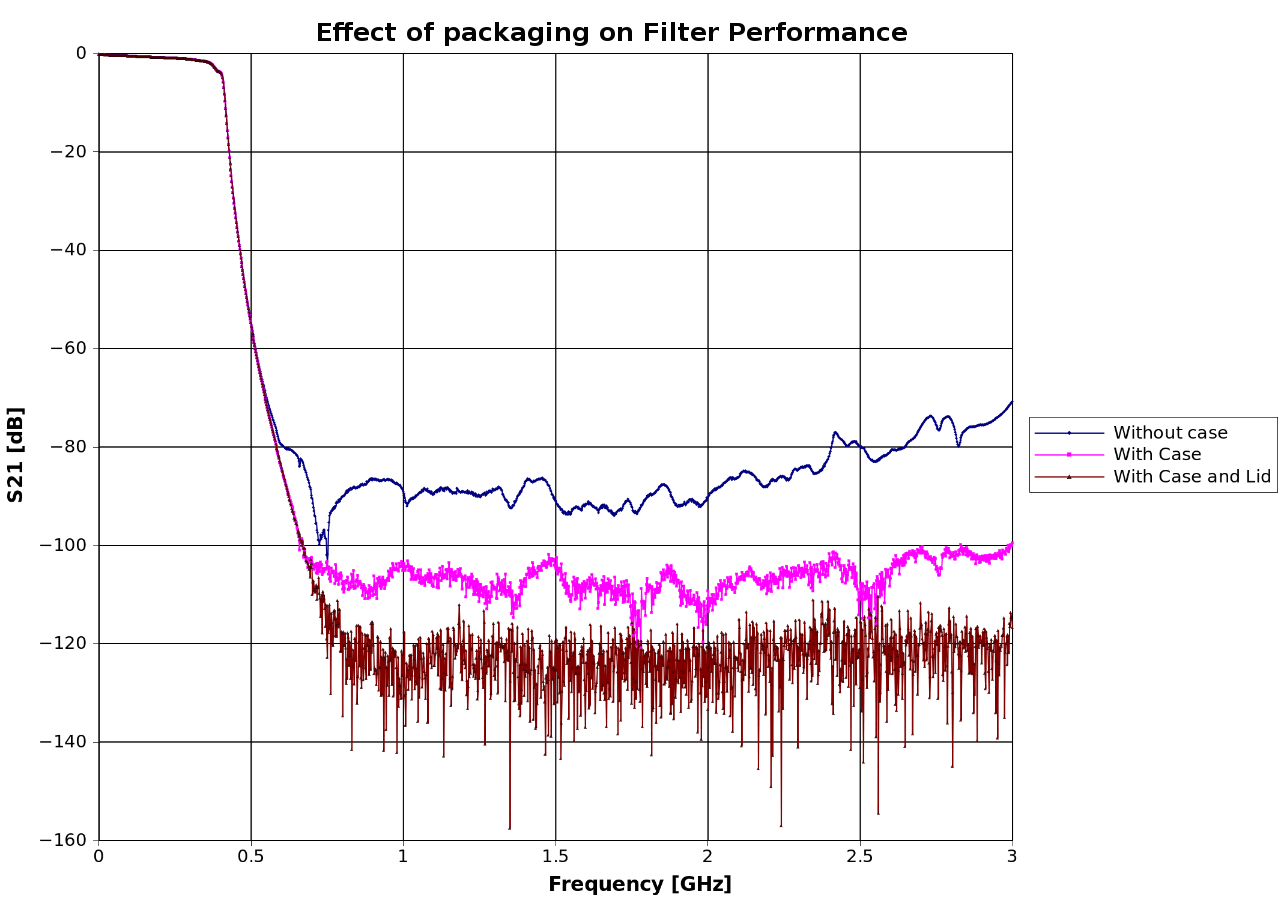
\includegraphics[width=\textwidth]{./images/LowFrequencyFilters/filterBoxing.png}
 % filterBoxing.png: 1319x930 pixel, 72dpi, 46.53x32.80 cm, bb=0 0 1319 930
 \caption{Comparison of different stages of the Filter construction process. These plots show the importance of properly enclosing the filter boards}
 \label{fig:filterBoxing}
\end{figure}

\begin{figure}
 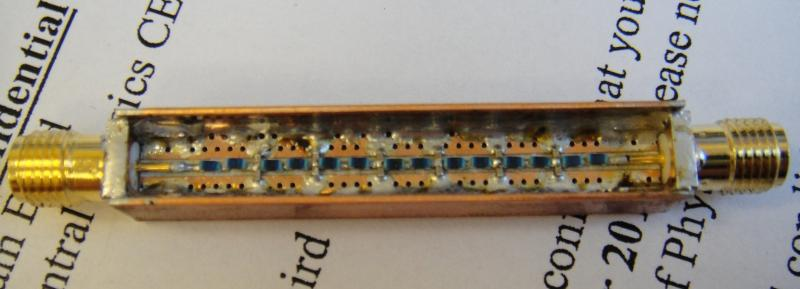
\includegraphics[width=\textwidth]{./images/LowFrequencyFilters/DSC03823a.jpg}
\caption{Final low frequency filter built into compact box. Notice the symmetry in the placement of components. The complete filter features a copper lid soldered into place completely sealing the unit. We have found that the boxing and lids are very important for optimal filter performance, as is apparent from \fign{fig:filterBoxing}. Also notice the solder joint between the PCB and the box wall. This reduces high frequency resonance artifacts, presumably caused by the (otherwise) exposed cavity}
\end{figure}

 

  \subsection{Performance}



\section{Double Sideband Mixers}

  \subsection{Design and Component Choice}

  \subsection{Performance}


\section{DC-6GHz Amplifiers}
Post down conversion gain is required to provide a suitable signal level at the ADC input. 


  \subsection{Performance}

  \subsection{Component Choice}

 \subsection{Wideband Biasing Chokes}

 \subsection{DC Blocking Capacitors}
DC blocking capacitors need to behave like series shorts in the frequency of interest. Capacitors can be modelled as a capacitor in series with a small, parasitic inductance and parasitic resistance \cite{Urs2011,broadbandCaps,Cain2010}. The impedance is then given by the equation in \eqn{eq:capacitorReactance}. This needs to be low (typically less than 1~ohm) across the frequency range of interest.

 \begin{eqnarray}
  X_{cap}=1/(2 \pi fC) + j 2 \pi fL + ESR
 \label{eq:capacitorReactance}
 \end{eqnarray}

Using \eqn{eq:capacitorReactance} large capacitor values are required for low frequency operation, while high frequency operation is limited by the parasitic inductance. 

As an example, at 5~MHz operation, a 100~nF capacitor has a reactance due to capacitance of 0.3~ohms, and a negligible 0.03~ohms contributed by typical parasitic inductances (0603 packaged MLCC capacitor has a typical parasitic inductance of 870~pH \cite{Cain2010}). However at 6~GHz the situation is reversed. The parasitic inductance now contributes 33~ohms, with the capacitance contribution of 0.0002~ohms being entirely negligible. The parasitic inductance is largely caused by the geometry of the package, with larger packaged featuring greater parasitic inductance. 

In order to achieve wideband performance from DC to 6~GHz, wideband DC blocking 0402 capacitors from American Technical Ceramics were used \cite{atc550L104}. The datasheet claims SRF of up to 40~GHz.

  
\section{Low Noise Amplifier Power Supply}

After the decision to move from the Jodrell Bank LNA's to Low Noise Factory LNA's, we required a means of powering the LNA's. Low Nois Facory do supply power supply units, however these do not allow remote monitoring. As such we built our own power supply units, in consultation with Low Noise Factory.

Extensive care was taken in components choice in order to minimise long term bias drifts. Many improvements were made in the original Low Noise Factory design, with particular care being taken to reduce any possible temperature drifts.

The basic schematic of the current source used in the power supply is included in 


\begin{figure}[ht]
 \centering
 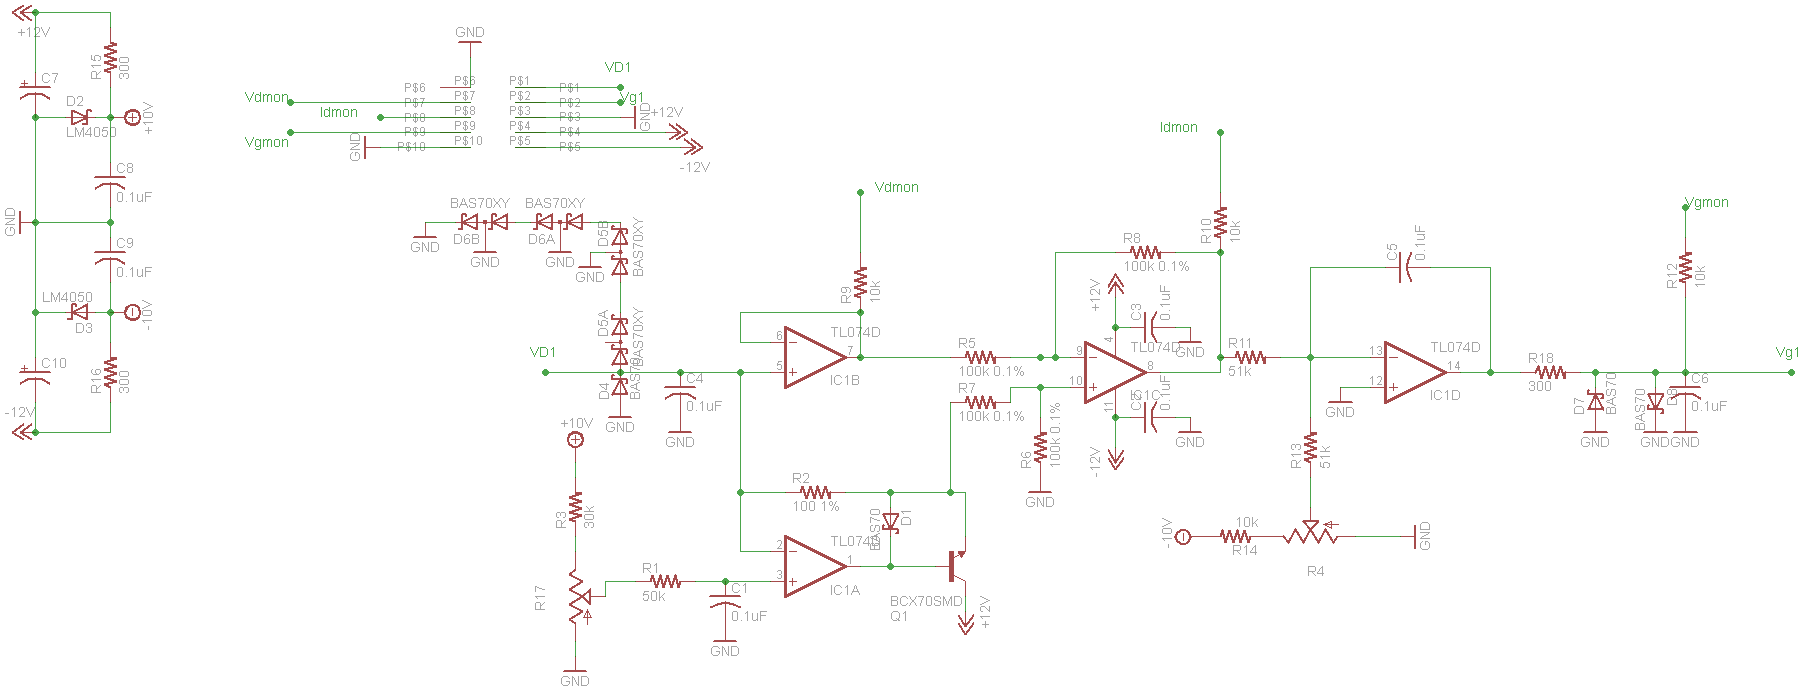
\includegraphics[width=\textwidth]{./images/LNAPSU/LNF-PS2_schematic.png}
 % LNF-PS2_schematic.png: 1807x692 pixel, 150dpi, 30.60x11.72 cm, bb=0 0 867 332
 \caption{The original amplifier power supply schematic. $\pm$10V reference was supplied by LM4050 Zener diode references (thermal stability 50ppm/\degc \cite{lm4050}), and TL074D opamps (Vo\approximately3000uV $\Delta$V$_{OS}$/$\Delta$C\approximately18uV/\degc \cite{tl074d}) were used for the gain and current stages . These were replaced by the more thermally stable REF195 voltage reference \cite{ref19x} and AD8624 opamps \cite{ad8624}. \fign{fig:lnaPSUNew} gives the schematic of the implementation. }
 \label{fig:LNFPowerSupply}
\end{figure}



\begin{figure}
 \centering
\subfloat[][New Power supply schematic]{
 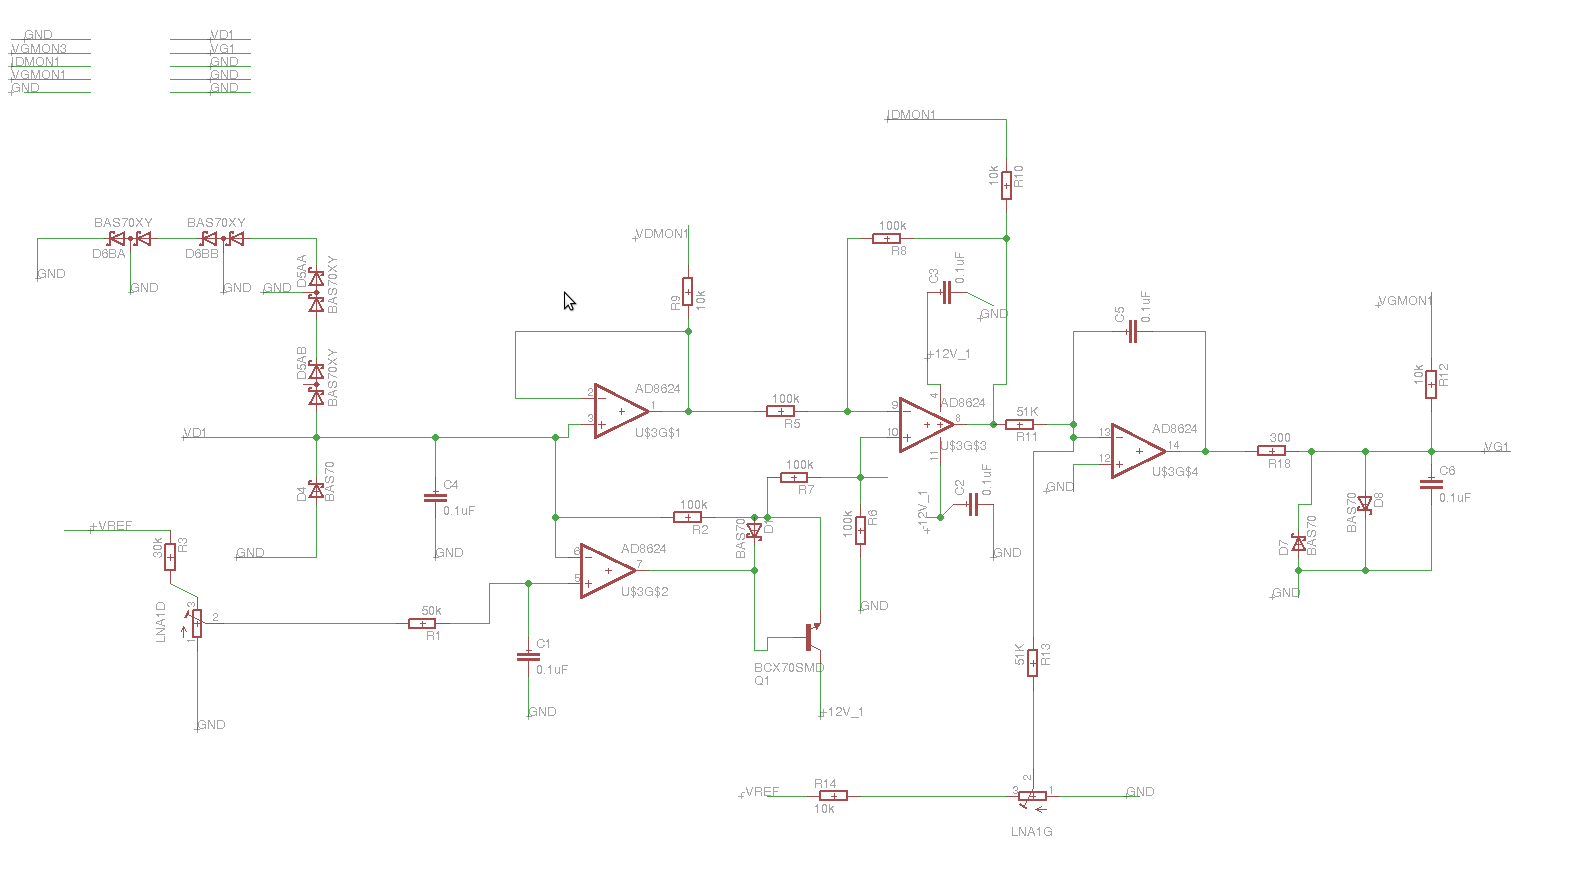
\includegraphics[width=\textwidth]{./images/LNAPSU/LNFNew.png}
\label{fig:NewPowerSupplyCircuit}
}\\
\subfloat[][New Reference voltage]{
 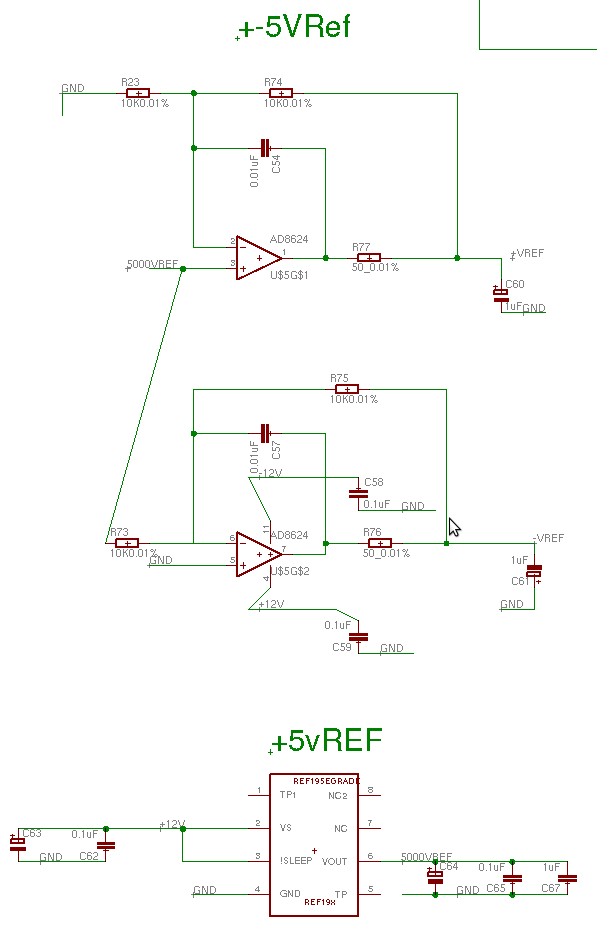
\includegraphics[height=0.4\textheight]{./images/LNAPSU/ReferenceSupply.png}
}\\

 % lowpass.png: 1357x340 pixel, 72dpi, 47.87x11.99 cm, bb=0 0 1357 340
 \caption{The updated-LNA Power Supply Board-The +5V reference voltage is provided by a REF195 E-Grade reference IC with a temperature coefficient of less than 5ppm/$^{\circ}$C \cite{ref19x}. The AD8624 opamps (Vo\approximately10uV $\Delta$V$_{OS}$/$\Delta$C\approximately1.2uV/\degc) \cite{ad8624} }
 \label{fig:lnaPSUNew}
\end{figure}







Replaced zener diode voltage reference generators, with REF19x units. Zener diodes 

\clearpage
\chapter{Receiver Testing}

\section{Introduction}
  \subsection{Order of Components}


\section{Load Stabilisation}
  \subsection{Cryocontrol}
\subsection{Bobbin Redesign}
\subsection{Temperature Sensor}


\section{RF and IF Band Definitions}




\begin{figure}[ht]
 \centering
\subfloat[Full Band measured by changing to 4GHz LO. This shows the low side rolloff. The steep slope after 1GHz is due to the power splitter frequency response.]{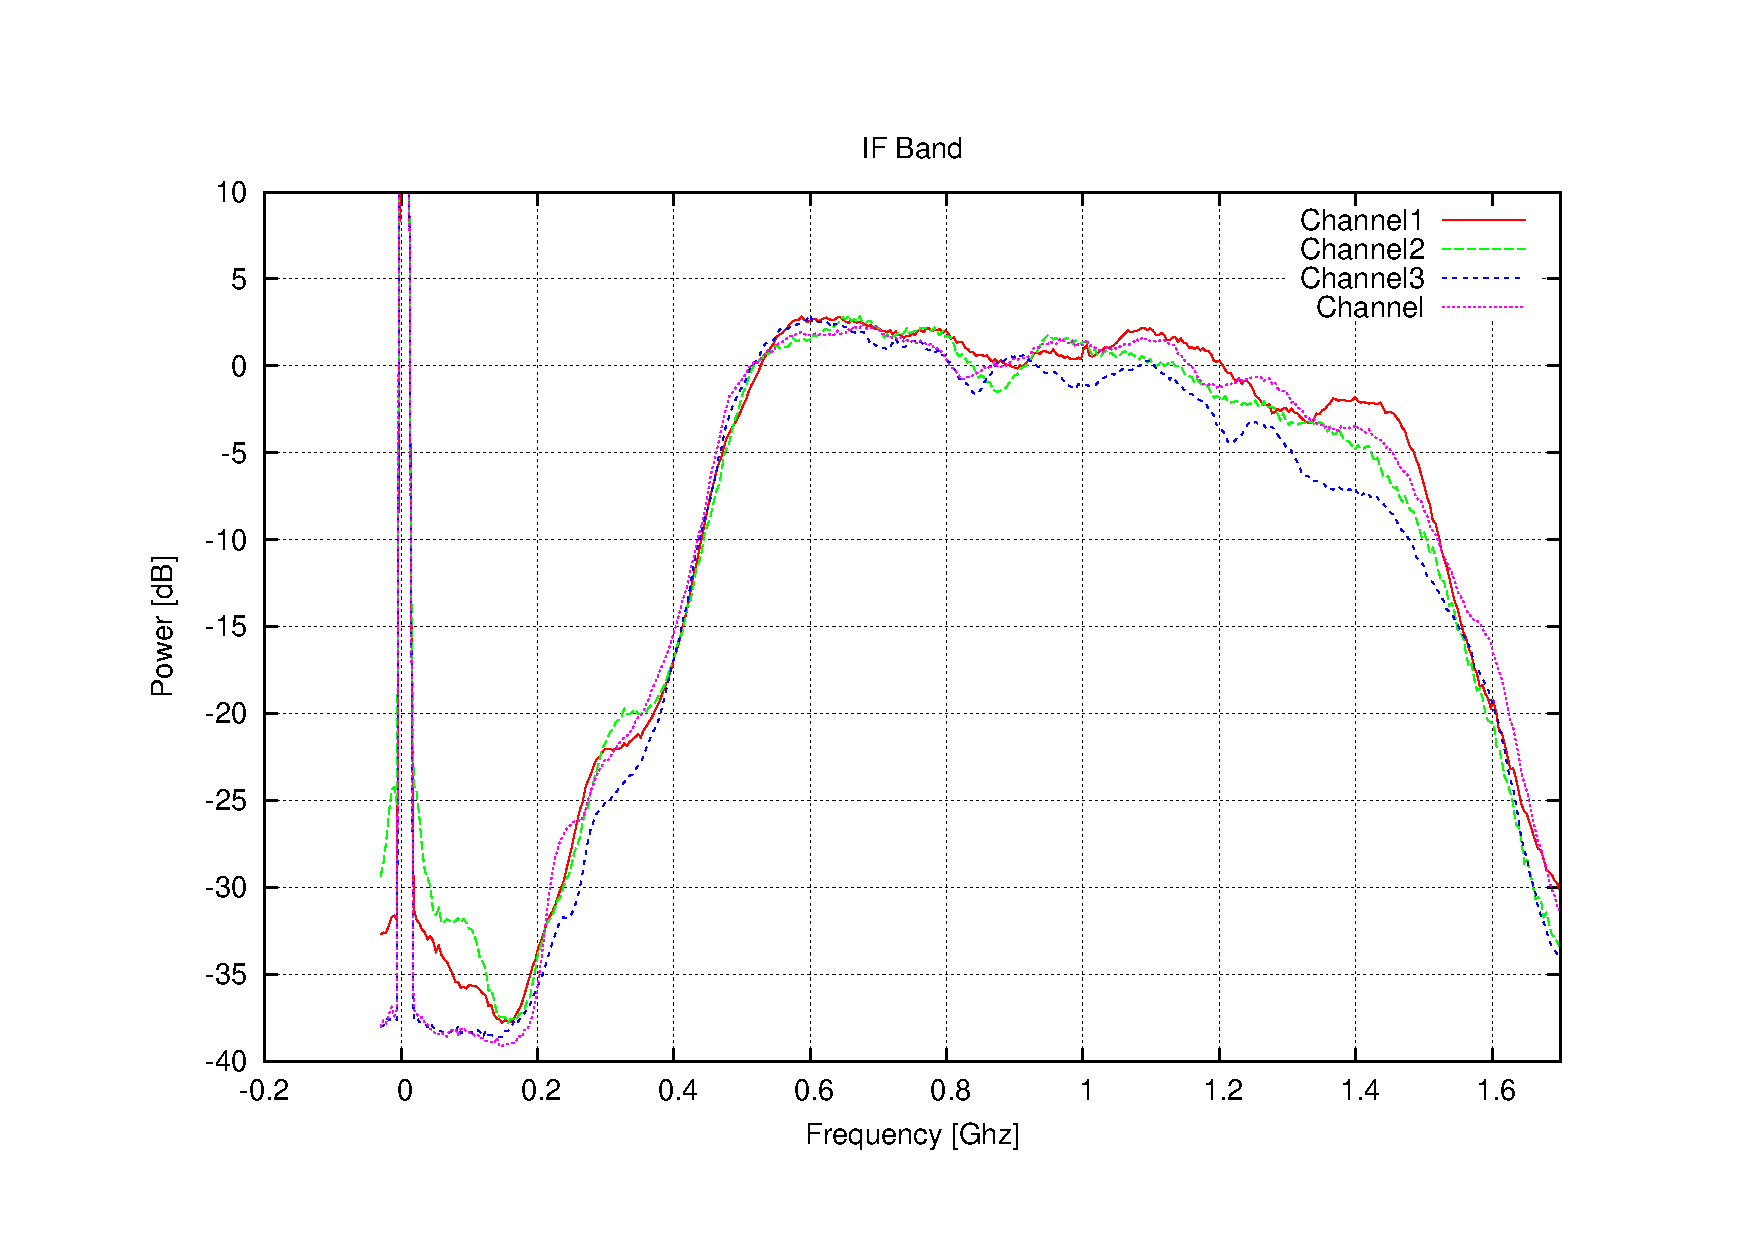
\includegraphics[width=0.4\textwidth]{./images/digitalReceiver/BandPassPlots/IFBandPass4GHzLO.pdf}\label{fig:IFBandDefinitions4GHz}}
\hspace{0.2cm}
\subfloat[The two digitised bands, DC$\rightarrow$500~MHz and 500$\rightarrow$1000~MHz]{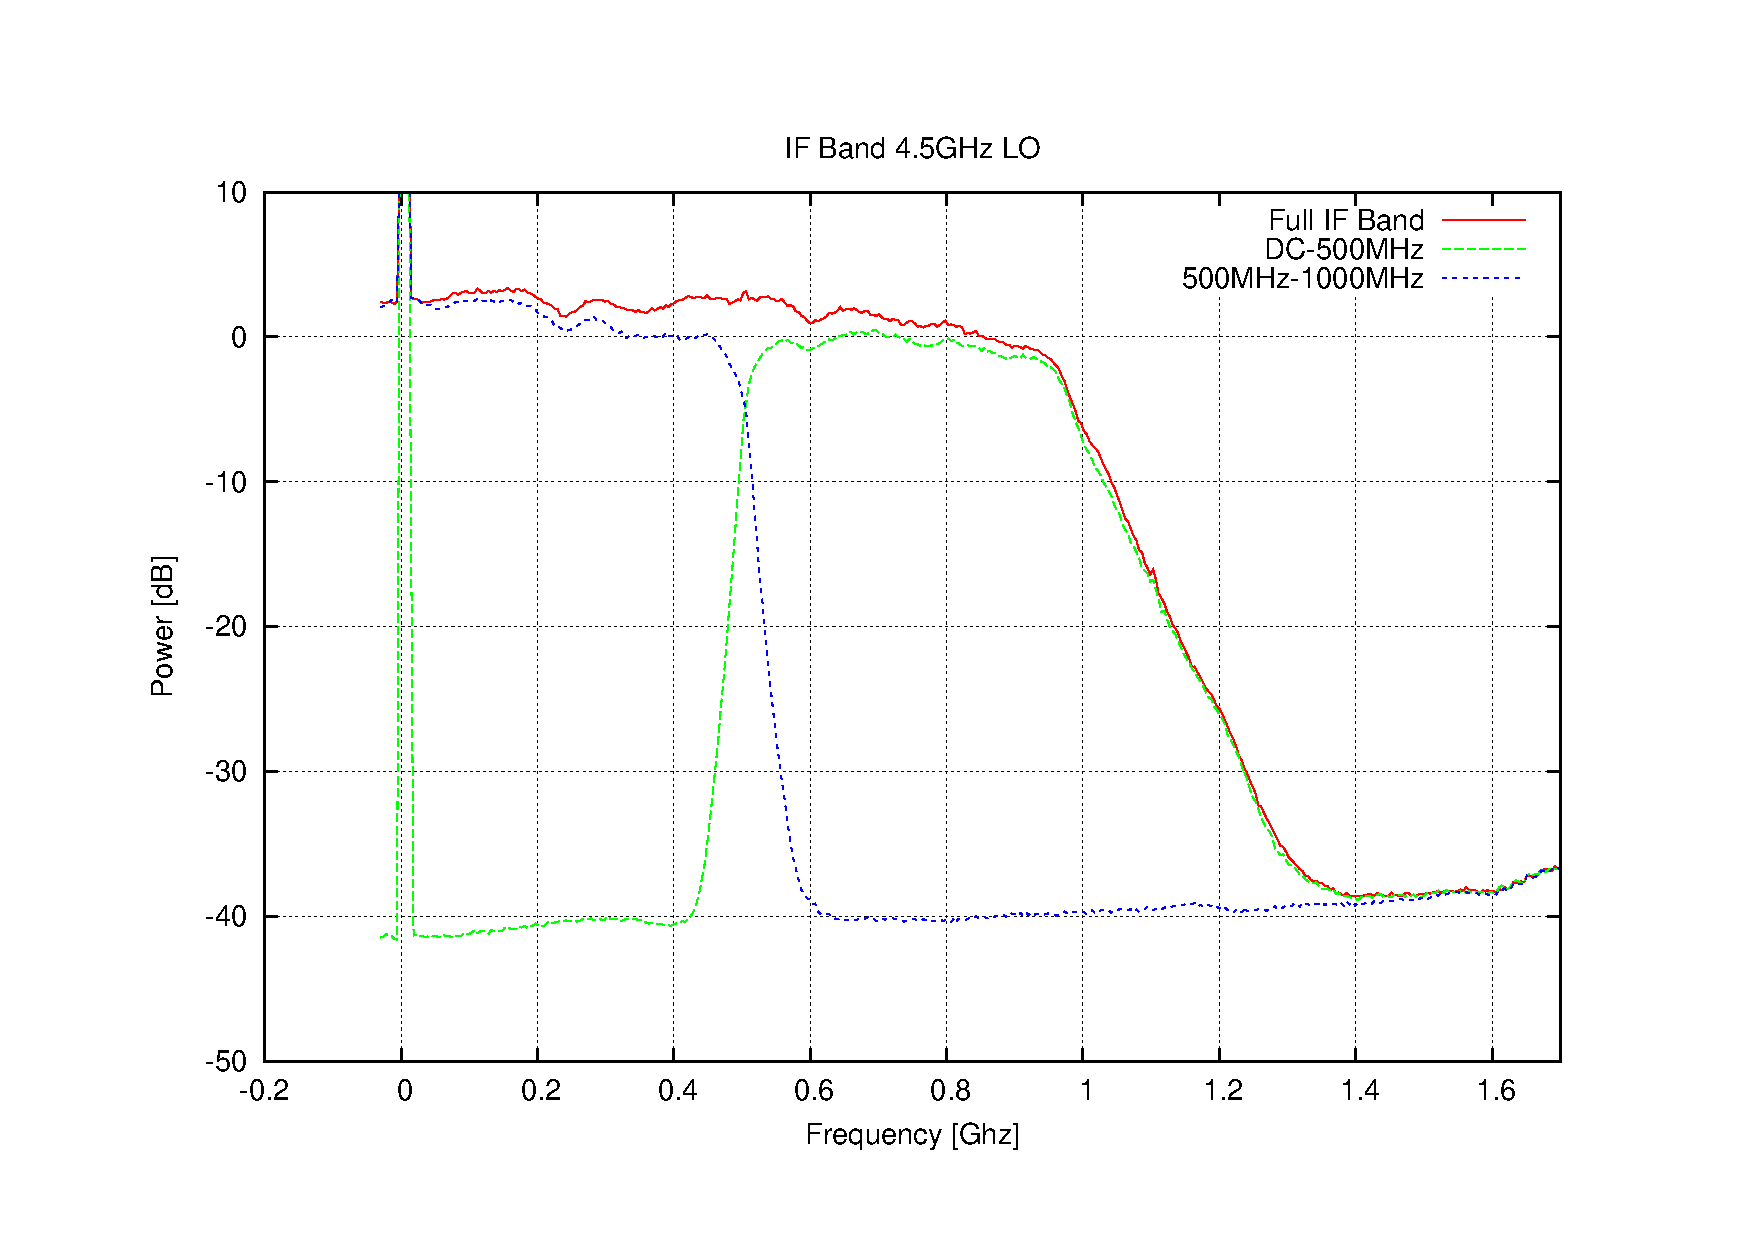
\includegraphics[width=0.4\textwidth]{./images/digitalReceiver/BandPassPlots/IFBandPass4_5GHzLO.pdf}\label{fig:IFBandDefinitions4.5GHz}}
\caption{Measurements of the IF Bands digitised by the iADC}
\label{fig:IFBandDefinitions}


\end{figure}




  \subsection{System Temperature}

\section{2-20GHz Amplifier System Tests}
  \subsection{System Temperature}

\section{DC-4GHz Amplifiers}

\subsection{Wideband Capacitors}

\subsection{Wideband Biasing Choke}

\section{Horn Tests}
  \subsection{Anechoic Chamber Measurements}


\section{Full System Tests}
  \subsection{Low Noise Amplifiers (LNA)}

\subsection{Cold Component Tests} 

\section{Design Improvements over Northern Frontend}

  \subsection{SuperSMA connectors}

  \subsection{Redesign RF route}

  \subsection{Thermal decoupling of temperature Load}


  


\clearpage
\chapter{The Southern C-BASS System}
C-BASS uses cassegrain optics- We did not know the shape of the primary reflector and needed to establish this.

\section{System Diagram}
  \subsection{Self-generated RFI considerations}
  \subsection{Remote Operations}

\section{Servo Control}

  \subsection{Description}

    \subsubsection{Requirements}
    \subsubsection{Hardware}
    \subsubsection{Software Integration}

  \subsubsection{Sensor Hardware Design}


    \subsubsection{Optical Pointing}


\section{Primary Dish Profile}
  \subsection{Photogrammetry}
\label{sec:photogrammetry}
Close range photogrammetry is a fairly recent innovation, which allows highly accurate measurements of large objects to be made in an fast, often automated fashion \cite{Luhmann2010}. Photographs are taken from different angles of targets placed in convenient positions on the object being measured. A few of the targets are geometrically coded (see \fign{fig:photogrammetryExampleOfPhotograph}), to ease the orientation of multiple photographs in post-processing . The positions of the individual targets can then be determined, with the accuracy varying as a function of camera resolution, target contrast, and separation angle. Accuracies of up to 1:250 000 are routinely quoted when using carefully calibrated equipment.  Fortunately,  the technique is suitable for use with high end consumer grade cameras \cite{Deng2001}, althought the expected accuracy is lowered.

We made use of this technique in order to characterise the donated Telkom dish.

\subsubsection{Target Choice}

The industry standard is to use retroflective targets. These generally take the form of black adhesive 'stickers' with reflective sections hand pasted into place. These can be expensive to manufacture and put into position.

In the name of completeness and frugality, we also experimented with a slightly unconventional approach, by projecting a series of targets onto the dish surface from a data projector. As can be seen in \fign{fig:photogrammetryExampleOfPhotograph}, this allows a higher density distribution of points across the surface, and is significantly less expensive and time consuming to implement. 

However this technique suffers from a few obvious limitations, namely resolution and contrast. By fitting centroids to a target position, photogrammetry routinely achieves sub-pixel resolution in the point's position. Poor resolution and low contrast adversely effect this process, to such and extent that we were unable to get a well constrained solution using the projected targets, and after many less than glamourous nights, decided to use the industry standard retroreflective targets. 


\begin{figure}[ht]
 \centering
 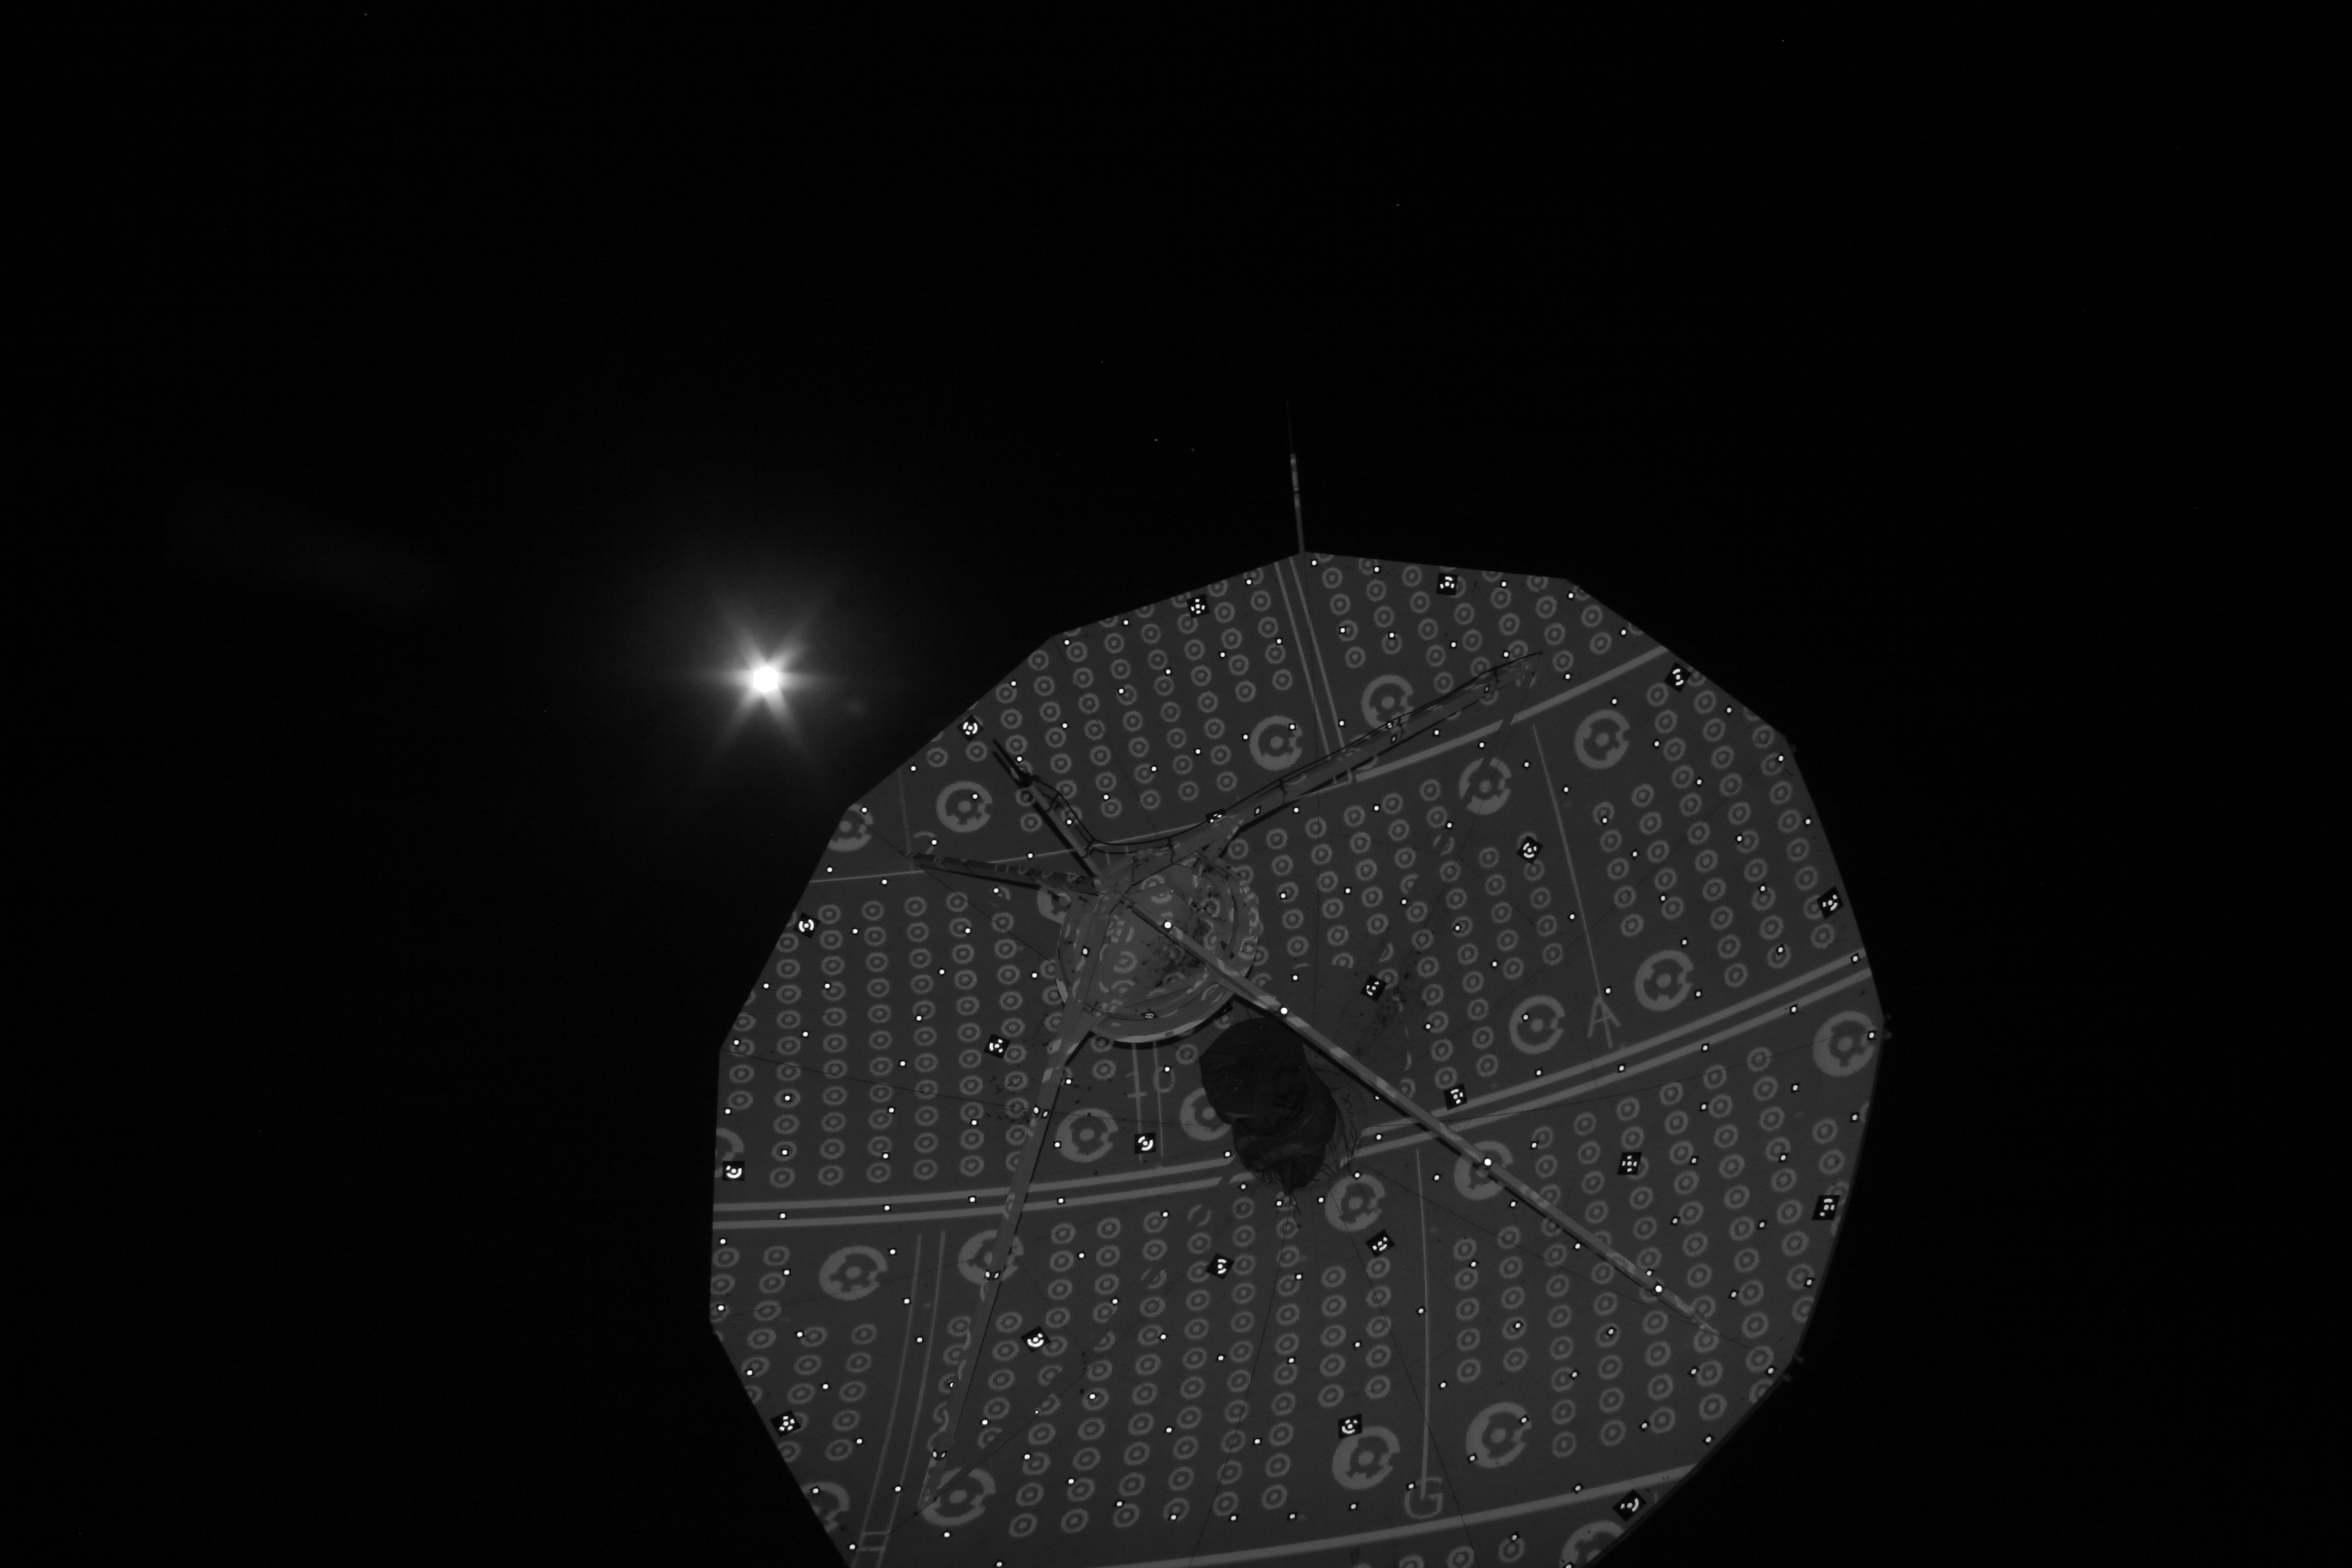
\includegraphics[width=\textwidth]{./images/photogrammetry/PhotoExamples/projectedAndRetrofelctive.JPG}
 % projectedAndRetrofelctive.JPG: 3504x2336 pixel, 72dpi, 123.61x82.41 cm, bb=
 \caption{An example of a photograph taken of the dish surface. The high contrast, bright points are retroflective targets, while the other (more densely distributed) points were projected onto the dish from a data projector. The targets consist of both standard circular targets, and geometrically coded targets to help in the post-processing photograph orientation.}
 \label{fig:photogrammetryExampleOfPhotograph}
\end{figure}

\subsubsection{Primary Shape}
The primary surface is not a 'strict' paraboloid, but rather falls into the category of 'shaped optics'. This type of design features an offset from the traditional parabolic reflector described in detail in \citeasnoun{Galindo1964}, and is a technique used to optimise the aperture efficiency of antennas.

\begin{figure}
 \centering
 \subfloat[Section through the dish surface relative to best fit parabola]{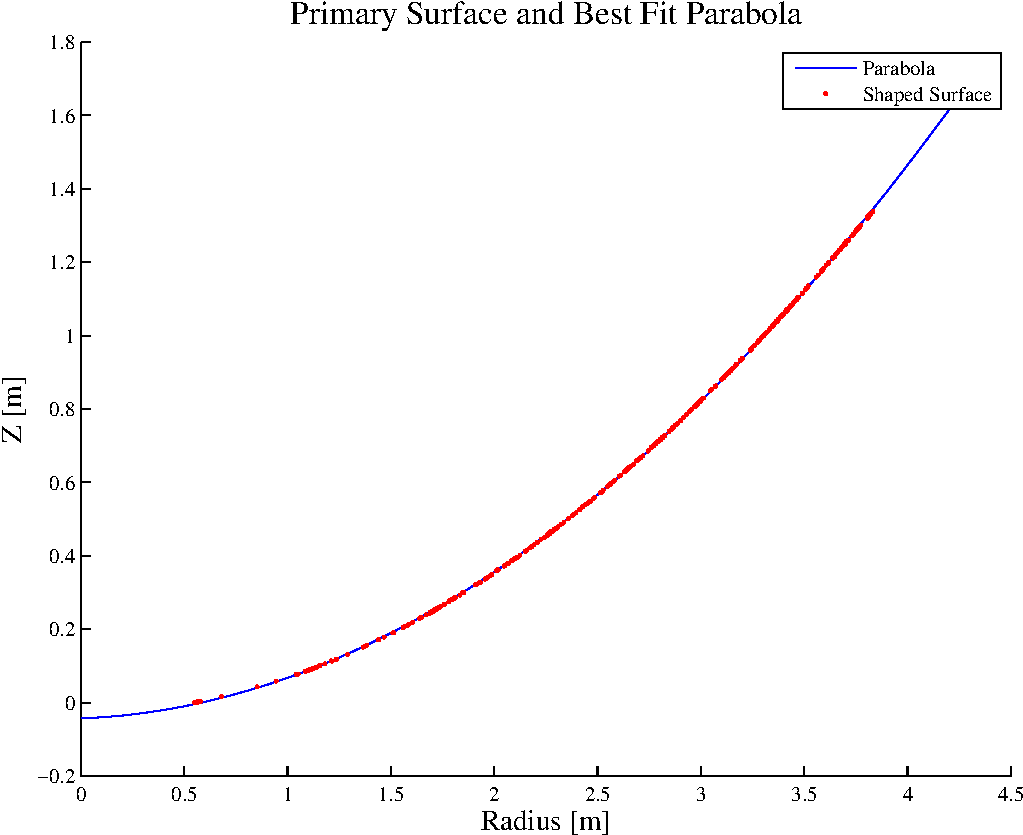
\includegraphics[width=0.4\textwidth,height=0.25\textheight]{images/photogrammetry/section.pdf}}
\hspace{0.2cm}
 \subfloat[Exaggerated (x20) section difference from the best fit parabola to show the shaping of the primary]{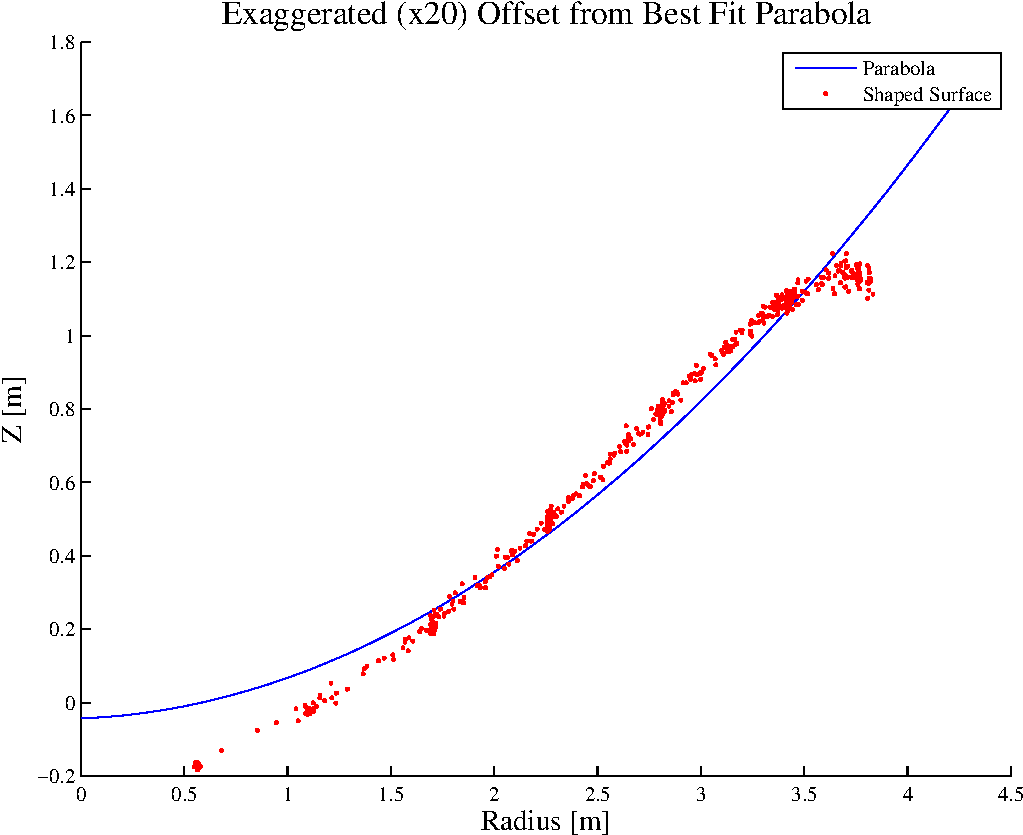
\includegraphics[width=0.4\textwidth,height=0.25\textheight]{images/photogrammetry/offset_section.pdf}}\\
 %\subfloat[Colour shows deviation from best-fit parabola when viewing the dish face on]{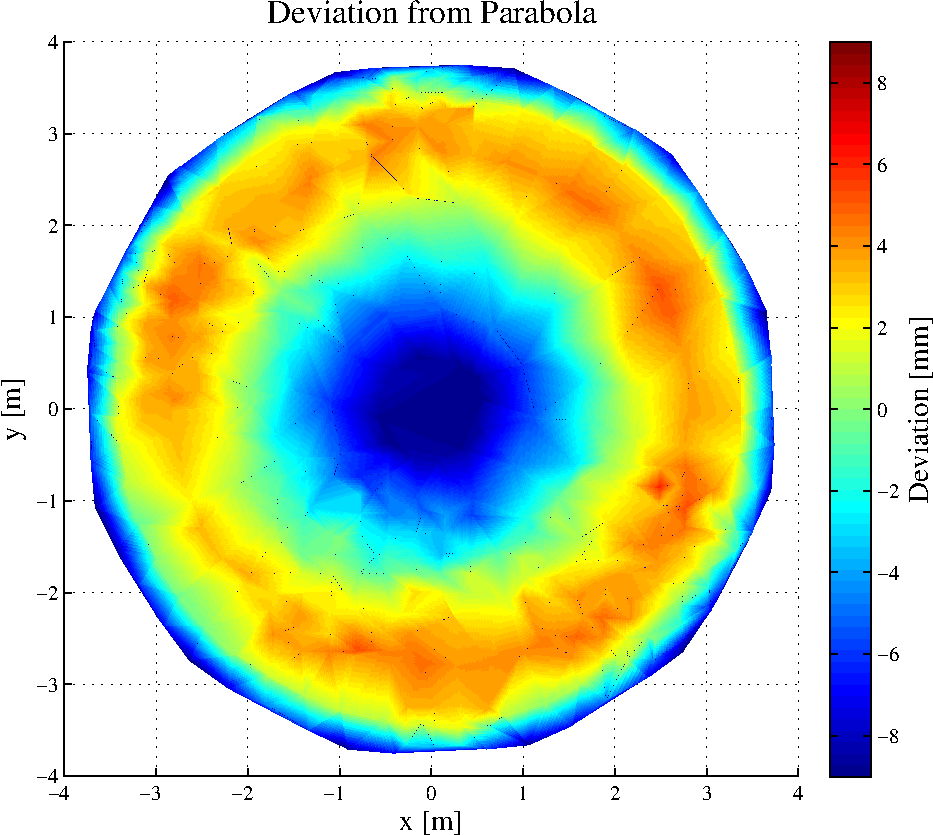
\includegraphics[width=0.4\textwidth,height=0.25\textheight]{images/photogrammetry/shape.pdf}}\\
 \subfloat[Colour shows the deviation from model used in optical design before transport- RMS=1.61~mm ]{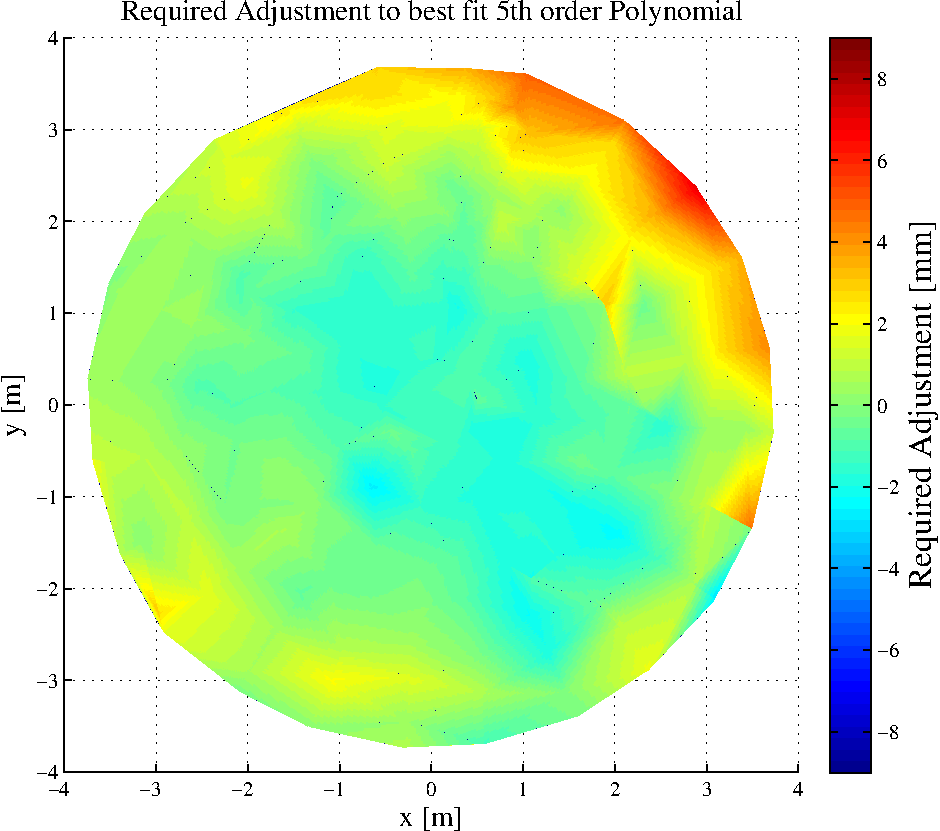
\includegraphics[width=0.4\textwidth,height=0.25\textheight]{images/photogrammetry/before.pdf}\label{fig:before_transport}}
\hspace{0.2cm} 
\subfloat[Colour shows the deviation from model used in optical design after transport- RMS=3.91~mm ]{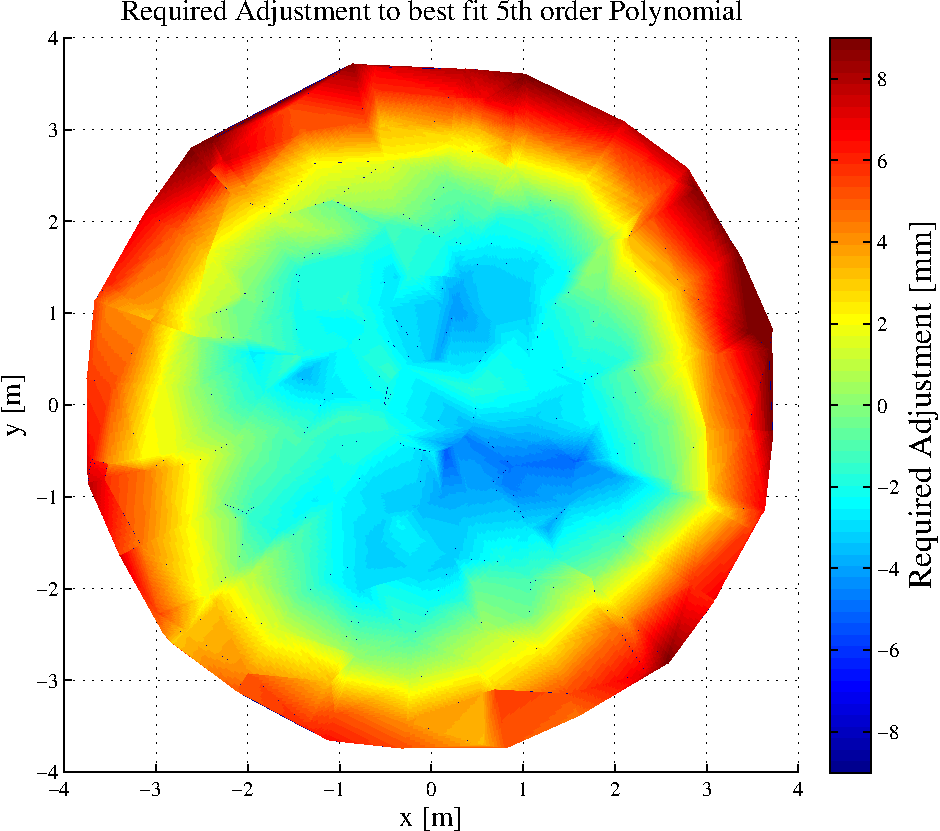
\includegraphics[width=0.4\textwidth,height=0.25\textheight]{images/photogrammetry/after.pdf}\label{fig:after_transport}}
 % newdish_upgrade.jpg: 1280x728 pixel, 72dpi, 45.16x25.68 cm, bb=
 \caption{Primary reflector offsets from design goal obtained from photogrammetric measurements of the South African 7.6~m dish. The primary shape used in the optical design is a 5th order polynomial fitted to the shape in (a) and (b). The offsets shown in (c) and (d) are with respect to this 5th order polynomial.}
 \label{fig:dish_surface}
\end{figure}



    \subsubsection{Transportation Quality Control}

\subsubsection{Independent Check of Photogrammetry and First Light}
\label{sec:first_light}
We used a modified 12~GHz receiver and custom designed rectangular feed horn \cite{meeks_1976} to observe powerful Ku Band Geostationary Satellites. A photograph of the assembled receiver is included in \fign{fig:feed}. It is possible to establish a focal point by scanning through a source and adjusting the position of the feed to maximise the observed power. At the position of maximum received power, the phase centre of the feed and the focal point of the antenna are coincident, providing a direct measurement of the antenna focal point. The results of this experiment are shown in \fign{fig:focal_point}. It is also possible (using ray tracing) to derive an expected focal point given the photogrammetric shape described in Section~\ref{sec:photogrammetry}. Comparing the measured and expected focal points (derived using the \textit{GRASP8} ray tracing software package), provides an independent check on the quality of the photogrammetry results.  

 The consistency between expected and measured focal point was very reassuring and confirmed our photogrammetry data. A diagram of the optical layout of the antenna is \fign{fig:optics}

\begin{figure}[ht]
 \centering
 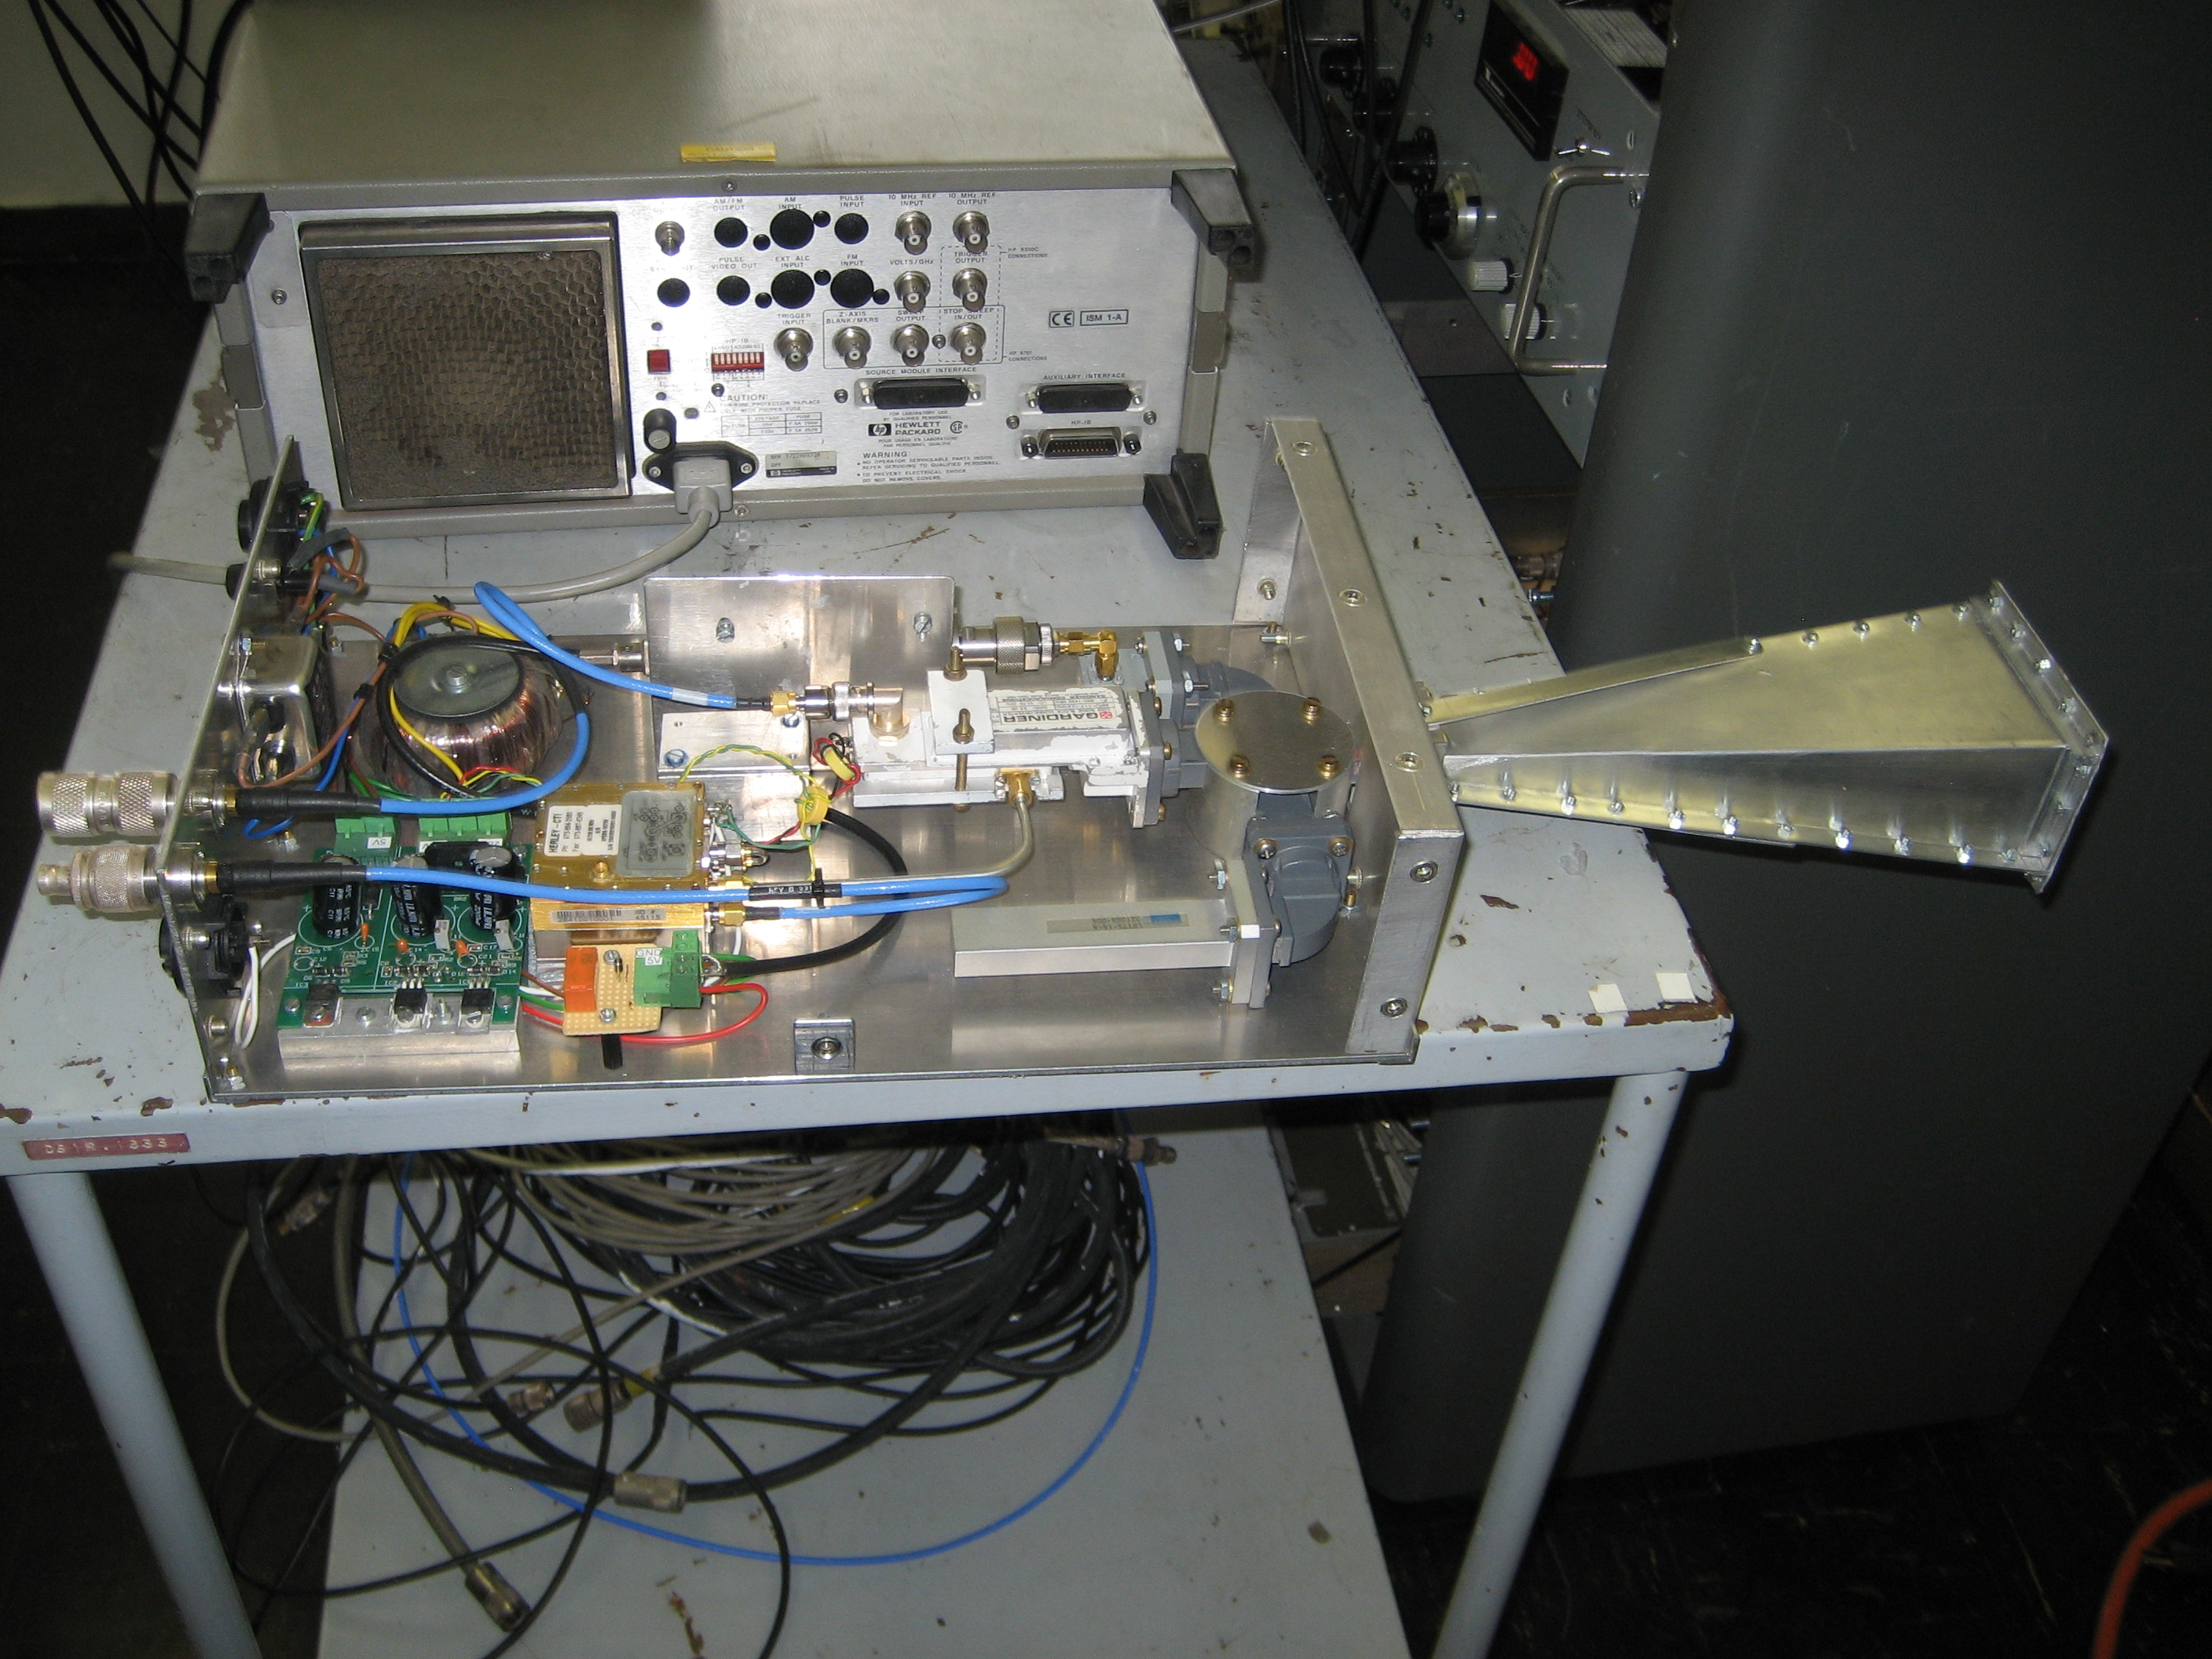
\includegraphics[width=\textwidth]{images/PAS7_cross_scans/img_1093.jpg}
 % img_1093.jpg: 2816x2112 pixel, 180dpi, 39.74x29.80 cm, bb=
 \caption{12~GHz Receiver and newly designed feed}
 \label{fig:feed}
\end{figure}

\begin{figure}[ht]
 \centering
 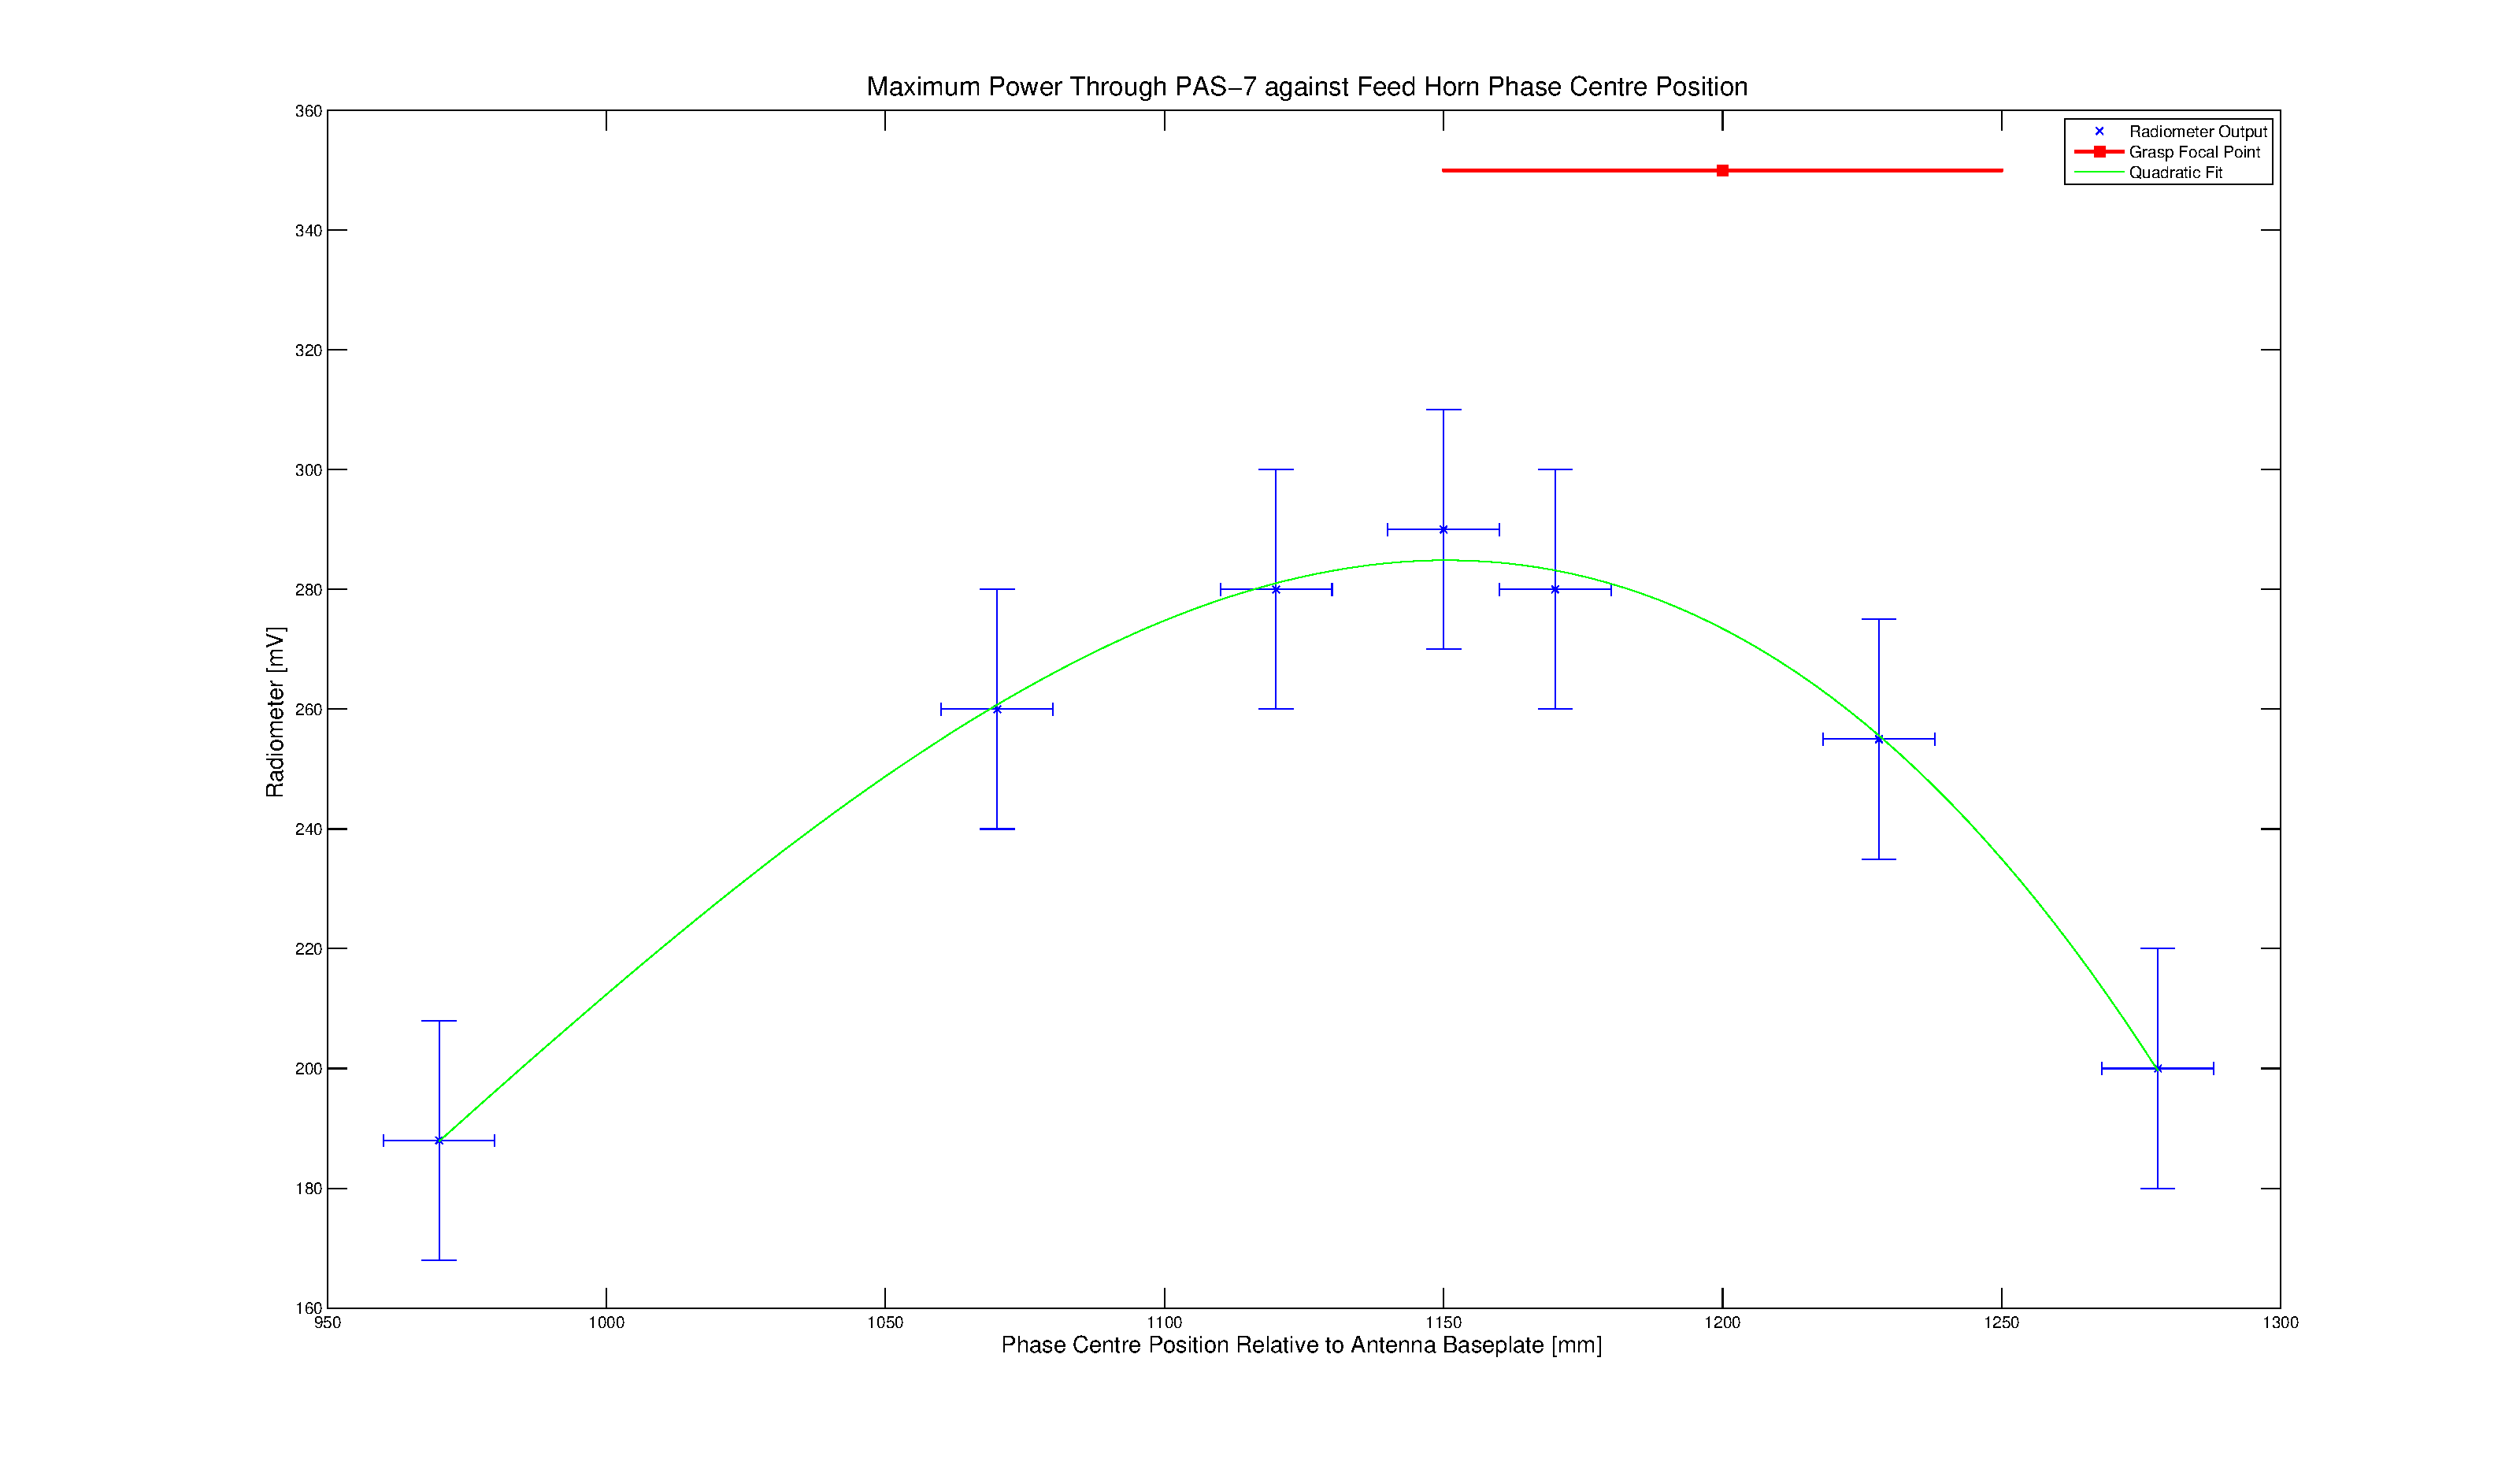
\includegraphics[width=\textwidth]{images/PAS7_cross_scans/focal_point.pdf}
 % focal_point.png: 1920x1076 pixel, 90dpi, 54.19x30.37 cm, bb=0 0 1536 861
 \caption{Maximum radiometer output voltage (which is proportional to RF power) when scanning through PAS-7, is plotted against feed phase centre position during the scan. The red marker shows the Grasp Software package prediction of the antenna focal point (1200$\pm$50~mm), calculated using the photogrammetry data of the primary and secondary reflector surface shapes. Maximum received power is expected when the feed phase centre and antenna focal point are coincident. The measurements show a maximum power at a feed phase centre position of $\approx$1150mm, which is (just) within the uncertainty of the Grasp simulation prediction of the antenna focal point (1200$\pm$50mm). Since the Grasp focal point is calculated using the photogrammetry data, this provides an independent 'sanity' check of the measurements used to design the new optics of the C-BASS antenna.}
 \label{fig:focal_point}
\end{figure}

\begin{figure}[ht]
 \centering
 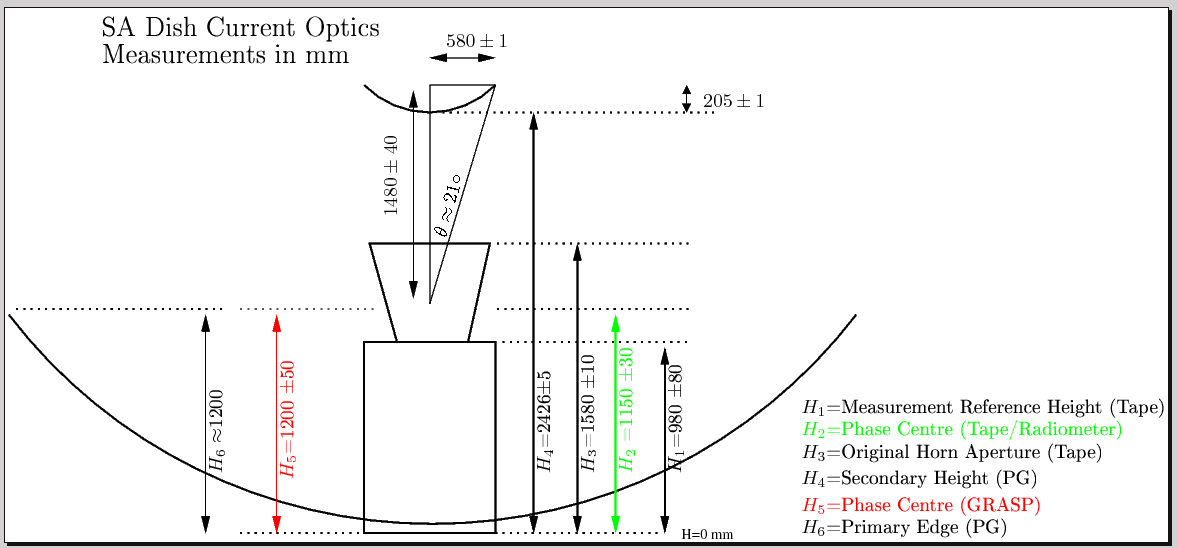
\includegraphics[width=\textwidth]{images/optics/optics4_after.png}
 % optics4_after.png: 1178x548 pixel, 98dpi, 30.53x14.20 cm, bb=
 \caption{Optics of the system before modifications- estimated uncertainties are approximate and not rigorously derived. Note this is the optical configuration prior to the redesign of the optics for the C-BASS experiment. These measurements are confirmed by both photogrammetry and the focal point check described in Section~\ref{sec:first_light}}
 \label{fig:optics}
\end{figure}




\section{Site Establishment}
\subsection{Infrastructure}
  \subsubsection{Power Provision}
  \subsubsection{Optical Fibre}
  \subsubsection{Access}
    \subsubsection{Control Shelter Considerations}
    \subsubsection{RFI Survey}


\subsection{Science Requirements}
  


 \clearpage
\chapter{Deploying the Southern Receiver}

\section{Strategy}
  

\section{Commissioning Observations}
  \subsection{Beam Patterns}
  \subsection{System Temperature}
  \subsection{Power Spectra}
  


 \clearpage
\chapter{Preliminary Data (if possible)}

\section{Science Project}
  \subsection{TBD:Galactic Centre?Spinning Dust Regions? deep CMB fields?}

  \subsection{Data Reduction}

  \subsection{Data Analysis}
  


  


 \clearpage
\chapter{Conclusisons}

\section{What's been done}

\section{What remains}
  


  


 \clearpage

%\section{Northern Hemisphere Data Pipeline}

\subsection{Data Format}

The final data output will be a full sky map presented in Healpix format as described by \citeasnoun{Calabretta2007}. This is a method of pixellating the sky into equal area pixels, and is commonly used in sky maps (for example WMAP).



\subsection{Data Pipeline}

% The switched signal (illustrated in \fign{fig:pseudo_correlation}) is sampled by an Analog-to-digital convertor (ADC) and 10~ms integrations performed by a field programmable gate array (FPGA). From the switched data it is possible to determine the the $T_{sky}$ - $T_{load}$ signal from the total intensity channels. The polarisation channels provide measurements of Stokes Q and U.

The data pipeline is currently being developed with the the processes (in rough sequence) including:

\begin{enumerate}
 \item Deglitching
 \item RFI excision
 \item 60Hz Mains Removal
  \item $\alpha$ correction for polarisation channel leakage 
 \item r factor correction to account for imbalance in temperature between cold load and sky (see \cite{Mennella:2003ii}
 \item Cold load corection fits for a sinusoidal (amplitude 1.9mK, frequency 1.2Hz) variation in the cold load temperature 
 \item Atmospheric Opacity Corrections
\end{enumerate}


An in depth discussion of these corrections is beyond the scope of this report. It is important to note that many of the steps listed, can be applied using different methods, with the optimal strategy is currently being decided upon. 

The data pipeline outlined above is implemented in MATLAB. Suitably calibrated and cleaned data is then written to FITS files, and passed on to the \textit{Descart} mapping suite (reference?). This suite of software is capable of destriping (extracting a 'true' signal for each pixel using multiple observations with different telescope parameters), however we are currently not utilising the functionality and are rather operating in the \textit{naive} software mode. This simply subtracts a mean bias offset, and averages the signal per Healpix pixel.

A current skymap of the data taken from OVRO is included in \fign{fig:northSkySurvey}. The map (in galactic coordinates) shows evidence of non-uniform scanning (around the North Celestial Pole) and also clearly shows the work that is still required in calibrating the data. However, the map does show the galactic plane as well as more detailed structure. This is a positive early stage C-BASS result, although there remains considerable work to be done.



\begin{figure}
 \centering
 %\subfloat[Northern sky as measured by the OVRO antenna-low contrast]{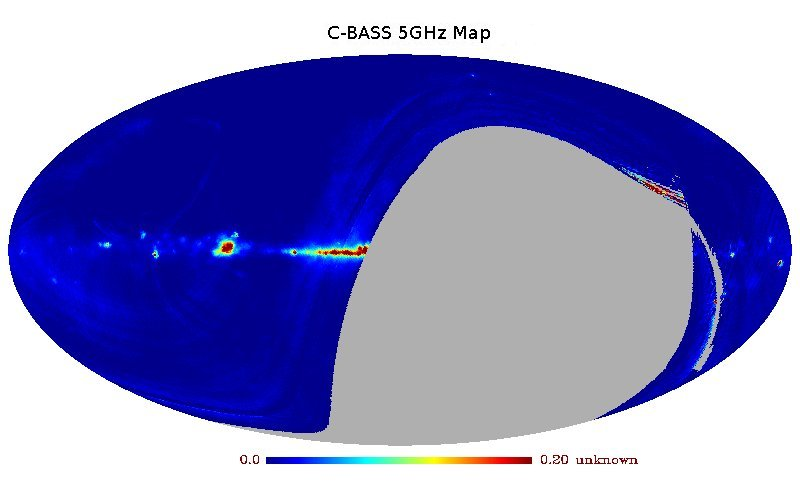
\includegraphics[width=0.4\textwidth,height=0.25\textheight]{images/maps/5GHz_2.jpg}}
%\hspace{0.1cm}
 %\subfloat[Northern sky simulated by Clive Dickinson- approximately same colour scale as in (a) ]{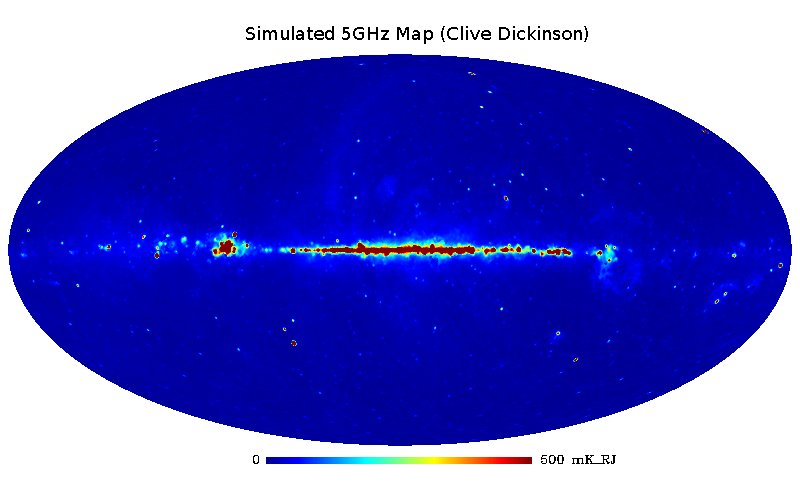
\includegraphics[width=0.4\textwidth,height=0.25\textheight]{images/maps/5GHz_coadded_500.jpg}}\\
 \subfloat[Increasing the contrast of the OVRO data shows significant calibration issues]{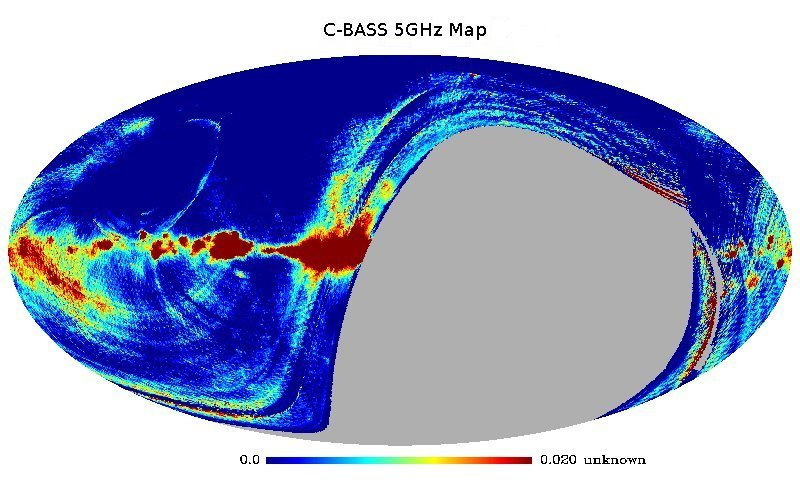
\includegraphics[width=0.4\textwidth,height=0.25\textheight]{images/maps/5GHz_02.jpg}}
\hspace{0.1cm}
 \subfloat[The simulated map on a similar intensity scale as in (c) shows the structure that we expect]{\includegraphics[width=0.4\textwidth,height=0.25\textheight]{images/maps/5GHz_coadded_80}}

 % newdish_upgrade.jpg: 1280x728 pixel, 72dpi, 45.16x25.68 cm, bb=
 \caption{Current state of Northern Sky maps (in Galactic Coordinates). Note that since we haven't yet introduced an absolute calibration scale, the comparisons between our data and simulated data are approximate.}
 \label{fig:northSkySurvey}
\end{figure}

% \begin{figure}
%  \centering
%  \includegraphics[width=\textwidth]{./images/descart/destriping.png}
%  % destriping.png: 1920x1200 pixel, 72dpi, 67.73x42.33 cm, bb=0 0 1920 1200
%  \caption{Illustration of destriping data (Joe Zuntz private communication)}
%  \label{fig:destriping}
% \end{figure}


 

\subsection{Noise Diode Stability and Linearity}

\fign{fig:northSkySurvey} shows the importance of proper calibration. Many of the choices available to us in calibrating the data rely on injecting a well understood noise diode signal. The long term stability of the noise diode is particularly important in this.

To this end we have begun a process of monitoring the noise diode against bright calibration sources. The resulting data from scans against CasA and TauA are shown in \fign{fig:calCheck}. These scans have been optimised to allow the following checks:

\begin{enumerate}
 \item Noise Diode linearity
 \item Pointing
 \item Noise diode stability
 \end{enumerate}

The noise diode linearity is easily check by comparing the noise diode contribution to the signal while off source, against the contribution while on source. If the noise diode is in a linear region, the relative contributions should be the same. Pointing is checked by fitting a gaussian to the azimuth and elevation cross scans. This pointing 'sanity' check is critical, as even small pointing errors will effect the measured flux, and hence our ability to check the noise diode stability. For the stability we can simply compare the noise diode signal to source signal over a period of time. Since the time between the noise diode event and calibration scan is short, any variations in receiver gain or atmospheric contributions are  common to both. 


\begin{figure}
 \centering
\subfloat[CasA used to check detector diode linearity and long term stability of the noise diode]{\includegraphics[width=\textwidth,height=0.7\textheight]{./images/calibration/casALabelled.pdf} \label{fig:casACal}}
\hspace{0.2cm}
%\subfloat[TauA used to check detector diode linearity and long term stability of the noise diode]{\includegraphics[width=\textwidth,height=0.35\textheight]{./images/calibration/tauA.pdf} \label{fig:tauACal}}
\caption{Long term noise diode stability observations. These show the check for the linearity of the detector diode (\textit{Diode Slope}) by comparison between the two noise diode events and the antenna pointing check performed on  the CasA. This is a bright, point sources in the 0.8$^{\circ}$ C-BASS beam. This shows evidence for detector diode non-linearity, with the slope of the diode output decreasing by $\approx$ 2.7\%. The first noise diode event is triggered with the telescope at the same elevation as the source but with an offset of 5$^{\circ}$ in azimuth. If the time between Noise Diode Event \#1 and the azimuth cross scan is short and at the same elevation as the source (i.e receiver gain fluctuations and atmospheric effects are negligible), and the pointing is accurate, it is possible to calibrate the noise diode signal against the source, and check the long term stability of the noise diode.  }
\label{fig:calCheck}

\end{figure}




 \clearpage
%\section{Summary and Timeline}

\subsection{Control and Data Acquisition}
In October of 2010, I spent some time at the South Africa C-BASS beginning integration of various systems. The primary focus of this trip was to set the antenna up for control under the Owens Valley control system, so as to keep the systems identical. 

The trip was a success and the South African antenna is now usable with the OVRO control system. Optical pointing was undertaken to test the control system, and we were able to achieve pointing errors of less than $1'$~rms. This was detailed in a previous report. 

We are currently working on a similar integration of the new digital backend.

\subsection{Backend}

The digital backend is currently undergoing full testing, preliminary results have shown it to be functional. Rotating the polarisation angle of input test signals produce expected rotation of Stokes U into Stokes Q. 

\subsection{RF Chain}
All components have been manufactured except the Low Noise Amplifiers (LNA's) and the $500\rightarrow1000$~MHz bandpass filters. The LNA's have been a major problem, but they should be ready by the end of October for full system integration. We are confident that the next iteration of the bandpass filters will perform adequately. All other post-cryostat RF components have been built, and tested using the digital backend.

\subsection{South African Infrastructure}
The following are in place:
\begin{itemize}
 \item Antenna
 \item Power
 \item Fibre
\end{itemize}

We still need to design and build a shielded box to house the electronics in (due to strict RFI policies in place for the final deployment location). We also need to procure a water chiller (for cooling the Helium Compressor) and a vacuum pump. This process has begun and we have quotes for these.



\subsection{Timeline}


Once C-BASS is deployed and commissioned, the survey will take a minimum of 8~months. This is the survey time I have used in the timeline below.
\begin{itemize}
 \item \textbf{September 2011} : Complete integration of ROACH with control software. Finalise RF chain (with regard to position of 2 way splitters). Complete assembly of $500\rightarrow1000$~MHz bandpass filter. Order Vacuum pump and water chiller. Assemble additional broadband amplifier plate.
 \item \textbf{October 2011} : Integrate C-BASS frontend i.e OMT, Linear to Circular, $180^{\circ}$ hybrids, couplers, and low noise amplifiers.
 \item \textbf{November 2011} : Bring assembled C-BASS frontend to Oxford for commissioning with ROACH backend. Test complete RF assembly on Oxford roof.
 \item \textbf{December 2011} : Probably away
 \item \textbf{January 2012} : Continue Oxford commissioning. Feed horn beam measurements in anechoic chamber, system temperature, system integration etc.
 \item \textbf{February 2012} : Commissioning/Shipping
 \item \textbf{March 2012} : Deployment at Hartebeeshoek Radio Observatory (HartRAO). Begin integrated commissioning tests e.g beam pattern measurements, system temperature checks, remote operability etc.
 \item \textbf{April 2012} : Continue commissioning at HartRAO- focus on robustness and remote recovery of system.
 \item \textbf{May 2012} : Continue commissioning at HartRAO. Try to make sure that there is data that could be used in thesis if there are major problems in the transfer to Klerefontein.
 \item \textbf{June 2012} : Transfer receiver to Klerefontein site. Check system operation- begin survey.
 \item \textbf{July 2012} : Survey (Begin writing thesis with data obtained at HartRAO and commissioning data at Klerefontein)
 \item \textbf{August 2012} : Survey (Continue writing thesis)
 \item \textbf{September 2012} : Survey (Continue writing thesis with data obtained at HartRAO- possibly begin including survey data from Klerefontein)
 \item \textbf{October 2012} : Survey (Continue writing thesis. Begin including survey data from Klerefontein)
 \item \textbf{November 2012} : Survey continues. First draft of thesis. This draft will probably focus on commissioning data rather than survey data.
 \item \textbf{December 2012} : Revision of thesis to include latest survey data.
\end{itemize}



\section{Appendix}

If the Appendix is not included, the full document can be found at \url{http://www-astro.physics.ox.ac.uk/~Copley/confirmationReport/confirmation.pdf}




\clearpage\clearpage
%\clearpage
\section{Status Summary}

\subsection{Northern Hemisphere Survey}

The OVRO antenna design and installation has been completed with a similar design expected for the Southern Hemisphere antenna. The complete antenna is shown in \fign{fig:ovroTelescope}. We have currently agreed on a commissioning process, and are working towards completing this.






\subsection{Southern Hemisphere Survey}
Construction has begun on the secondary reflector. A new digital receiver will be used on the South African antenna (see Section~\ref{sec:digitalImplementation}). The digital design is complete, and we are currently sourcing the front end analog receiver components. The South African antenna is ready to begin observations after we install the complete system in September of 2010.

%\newpage
%\part{Previous Experience and Qualifications}
%\setcounter{section}{0}




\clearpage
\newpage
%\part{Intentions}
\setcounter{section}{0}















\appendix

\section{Stokes Parameters}
\label{sec:stokes}

It is important to describe polarisation, as it clarifies key considerations in the receiver design. \citet{tinbergen_1996} provides a good reference on the use of polarimetry in astronomy and was used extensively in the following summary. Detailed descriptions have been avoided.

An electromagnetic wave propagates in a transverse fashion and exhibits vector characteristics. At any instant, the vector describing the electric field can be resolved into two components at right angles to each other. For unpolarised radiation there is no lasting relationship between these two components. For polarised radiation, however, an amplitude and phase relationship does exist, such that the vector comprised of the two components traces out an ellipse, circle or straight line. These three states give rise to the terms \textit{elliptical, circular and linear} polarisation respectively.  

The Stokes parameters (I,Q,U and V) fully describe the state of polarisation. The parameter I characterises the intensity of the incoming radiation, Q and U characterise the state of linear polarisation and V the state of circular polarisation. Measuring I, Q, U and V at radio frequencies can be done by correlating orthogonal modes of the incoming radiation. 

\citeasnoun{tinbergen_1996} also points out the significant relationship, that left (L) and right (R) hand \textit{circular polarisation} the Stokes parameters are related to the correlations by 

\begin{eqnarray}
& I &= LL^{*} + RR^{*}  \label{eq:stokes_circ_I} \\
& Q &= 2Re(LR^{*}) \label{eq:stokes_circ_Q}\\
& U &= -2Im(LR^{*}) \label{eq:stokes_circ_U}\\
& V &= LL^{*}-RR^{*} \label{eq:stokes_circ_V}
\label{eq:stokes_circ}
\end{eqnarray} 

(where $LL^{*}$ denotes the auto-correlation of the left circular polarisation for example) while for X and Y \textit{linear polarisations} the parameters relate to the correlations by


\begin{eqnarray}
& I &= XX^{*} + RR^{*} \label{eq:stokes_lin_I} \\ 
& Q &= XX^{*} - YY^{*} \label{eq:stokes_lin_Q}\\
& U &= 2Re(XY^{*}) \label{eq:stokes_lin_U}\\
& V &= 2Im(XY^{*}) \label{eq:stokes_lin_V}
\label{eq:stokes_lin}
\end{eqnarray} 

The significance of the equations is apparent when we consider the type of polarisation we are trying to measure. Since Q, U and V will be small percentages, it is preferable to use a form that produces measurements using correlation rather than the less sensitive differencing operation. We can see from the equations that equipment designed for measuring \textit{linear polarisation} (i.e Q and U) should use correlations of circular polarisation (as shown by Equation~\ref{eq:stokes_circ_Q} and Equation~\ref{eq:stokes_circ_U}), while equipment designed for measuring \textit{circular polarisation} (i.e V) should use correlations of linear polarisation (see Equation~\ref{eq:stokes_lin_V}). 


For C-BASS we are interested in Galactic polarised emissions. This will be dominated by the synchrotron radiation mechanism \cite{Reich:2006iq},\cite{Bennett2003} producing linear polarisation, hence we choose to use correlations of circular polarisation.


\section{Pseudo-correlation architecture}
\label{sec:pseudoCorrelation}
The polarimeter will be built using a pseudo-correlation architecture (see \fign{fig:pseudo_correlation} and \fign{fig:digital_receiver_mine}). This is a differential receiver architecture (with continuous comparisons between the sky temperature and a stable reference load, see \fign{fig:pseudo_correlation}) with the associated benefits of improved stability with amplifier gain fluctuations.  \citeasnoun{Mennella2003b} and \citeasnoun{Seiffert2002} describe this receiver architecture as implemented on the Planck-LFI instrument, and note the improvement over a a Dicke switched scheme (i.e switching between load and sky) by avoiding the need for an active switch in the receiver chain and improving the sensitivity by $\sqrt{2}$. 

We are currently using an analogue pseudo-correlation polarimeter for the OVRO antenna. The receiver consists of a front end cooled to 4~K. The cooled section comprises a ortho-mode transducer (OMT) which separates the incoming signal (defined hereafter as $T_{sky}$) into orthogonal linear polarisations, which are then converted to circular polarisation using 90\degt hybrids. The reason for the conversion to circular polarisation is described in Appendix~\ref{sec:stokes}. Each of the orthogonal circular polarisations (left (LHC) and right (RHC) hand circular polarisation) is then coupled to a reference load signal ($T_{ref}=4K$) through a 180$^{\circ}$ hybrid producing two signals ($T_{1}=T_{sky}+T_{ref}$ and $T_{2}=T_{sky}-T_{ref}$) which propagate through independent signal paths. In the first signal path, the signal passes through a phase switch applying a delay that alternates between 0 and 180\degt, while the other signal path is routed through a similar phase switch (for symmetry) with no change in phase being applied. The signals are then recombined (using a 180\degt hybrid in the Planck architecture) producing the output sequence in \fign{fig:pseudo_correlation}. The signals are then appropriately correlated to measure the Stokes parameters as described in \secn{sec:stokes}. In the new digital receiver the signals will be recombined in the frequency domain, after taking fast-Fourier transforms (FFT) of each of the signals independently. The correlations will then be implemented digitally.

This continuous comparison (again, see \fign{fig:pseudo_correlation}) between the sky and reference load temperatures is useful for removing gain fluctuations in the amplifiers, since fluctuations will effect both  $T_{sky}$ and the known $T_{ref}$ equally. In addition, the fast switching reduces the impact of 1/f (or pink) noise in the amplifiers \cite{Seiffert2002}). 



\section{Digital Implementation}
\label{sec:digitalImplementation}
The new digital receiver will perform a similar operation to the analogue receiver and will be implemented on a CASPER \textit{ROACH} board\footnote{http://casper.berkeley.edu/}. Two 500~MHz bands will be captured using 1~Gsps analogue-to-digital converters (ADC), after suitable heterodyning of the 4.5~GHz$\rightarrow$5.5~GHz frequency band into the 0$\rightarrow$1000~MHz band. The two 500~MHz bands are defined by a 0$\rightarrow$500~MHz low pass filter (first Nyquist zone) and a 500MHz$\rightarrow$1000~MHz band pass filter (second Nyquist zone) as depicted in the diagram in \fign{fig:digital_receiver} and \fign{fig:digital_receiver_mine}. A n=128 fast fourier transform (FFT) is performed by the \textit{Virtex-5} field-programmable gate array (FPGA) providing 64 channels ( i.e the real components of the n=128 FFT)  and a bin width  of 7.8~MHz per channel across each 500~MHz band. Increasing the spectral resolution further would only be possible on a larger FPGA.

\subsection{Advantages of the Digital Implementation}
The analog polarimeter is designed with a single 1~GHz band, with correlations performed using analog components (90  $^{\circ}$ and 180 $^{\circ}$ hybrids). A similar approach could be used in a digital receiver. The incoming data is sampled, and the analog components emulated with Hilbert transforms and correlating various signals.  


Significant improvement on this design can be achieved by performing the correlations in the frequency domain. The incoming signal is fast fourier transformed, and the correlations between signals are implemented as a multiplications. This is the approach we have chosen. The fast fourier transform channelises the data in 8~MHz wide bands, and operations occur on a per-channel basis. This approach is especially useful in radio frequency interference (RFI) detection and rejection. Since RFI is generally very narrow bandwidth ($\Delta f_{RFI}\ll$~8~MHz), it is unlikely to effect more than one of the 8~MHz wide spectral channels and can be robustly detected by a real time spectral kurtosis measurement. The effected channel can be discarded with loss of only ~1.5\% of the data during the period of the RFI contamination. In comparison, an analogue system requires discarding the entire time series effected by RFI.

Another advantage is the reconfigurability of the digital architecture. A new receiver can be implemented simply and easily, compared to analogue architectures. 


\begin{figure}
 \centering
 \includegraphics[width=\textwidth]{images/receiver_schematics/pseudo_correlation.png}
 % pseudo_correlation.png: 1920x1200 pixel, 72dpi, 67.73x42.33 cm, bb=
 \caption{The pseudo correlation architecture \protect \cite{Mennella2003b}. The diagram is relevant for one of the orthogonal polarisation states- in the receiver there will be two such signal paths for left and right hand circular polarisation respectively. } 
 \label{fig:pseudo_correlation}
\end{figure}


\begin{sidewaysfigure}
 \centering
 \includegraphics[width=\textwidth]{images/receiver_schematics/analogFull.png}
 % analog.png: 1920x1200 pixel, 72dpi, 67.73x42.33 cm, bb=
 \caption{The pseudo-correlation analog C-BASS radiometer/polarimeter designed by Dr. Oliver King and currently installed on the Owens Valley Antenna \protect \cite{King2009}. The 90\degt phase switch in the front,cold section, converts the linear polarised signal to circular polarised. The signal is then passed through the 180$^{\circ}$ hybrid, coupling in the load signal and amplified. The signal then splits into the radiometer and polarimeter sections. The radiometer signals are phase switched and passed through a second 180$^{\circ}$ hybrid producing a signal similar to that illustrated previously in \fign{fig:pseudo_correlation}. The polarimeter signals are passed through a 180$^{\circ}$ hybrid to remove the load signal, before phase switching and sampling.}
 \label{fig:analog_receiver}
\end{sidewaysfigure}


%\section{Filter Design}
\label{sec:filterDesign}
\subsection{Specifications}
The in-band RFI (\fign{fig:RFImaxHold}) is narrow band. Designing a notch filter to remove these signals requires a high quality factor (Q factor) ($Q=\frac{f_{c}}{\Delta f}$) design. A cursory examination of Figure~\ref{fig:RFImaxHold} suggests that each RFI band is approximately 25~MHz wide, which at 5~GHz requires a Q factor of 200. This is a challenging task, and can only realistically be achieved using superconducting filters, since most of the degradation in quality factor at this level is caused by resistive losses. Unfortunately, the timescales we were operating on did not permit a thorough exploration of superconducting filter options.

However upon more careful examination of Figure~\ref{fig:RFImaxHold}, it is clear that some relaxation of this requirement is possible, without significantly degrading the passband. Each of the major RFI bands (i.e 4.92~GHz and 5.18~GHz) has a second proximate RFI peak, which could be included into a single notch filter. To attenuate both of these a stop band of ~80~MHz is required (i.e Q factor of 63). This is an achievable goal on standard Copper printed circuit board, provided the copper is cooled to reduce resistive losses. A specification of 30~dB attenuation at the RFI frequencies was settled on.

\subsection{Design}

High Q filter design using microstrip, is usually accomplished using resonance structures placed parallel to a microstrip transmission line, with electromagnetic coupling between the two. The dimensions of these structures can be adjusted to resonate at the frequency of interest. Alternatively band pass filters can be constructed in a similar fashion by placing these resonating structures in series with the transmission line.

Since this was our first foray into the world of resonance filter designs we looked for a simple resonating structure which would be easy to 'tune'. The design we chose (\cite{splitRingClassic} )is shown in Figure~\ref{fig:squareRingResonator}.

\begin{figure}[ht]
 \centering
 \subfloat[Square Resonator]{\includegraphics[width=0.4\textwidth]{./images/NotchFilter/squareRingResonator.png} \label{fig:squareResonator}}
 \subfloat[Circular Resonator]{\includegraphics[width=0.4\textwidth]{./images/NotchFilter/circularRingResonator.png} \label{fig:circleResonator}}\\
 \subfloat[Manufactured Bandstop filter with a series of differently tuned square resonator structures]{\includegraphics[width=0.4\textwidth]{./images/NotchFilter/Design1.png} \label{fig:design1} } 
\subfloat[S21 Bandstop filter Result- See SRR plot]{\includegraphics[width=0.4\textwidth]{./images/NotchFilter/s21.png} \label{fig:s21design1} } 
 \caption{Possible resonance structures for the notch filter \cite{splitRingClassic}. These diagrams show the dimensions that can be adjusted. We chose to pursue the square type resonance structure \ref{fig:squareResonator}}
 % squareRingResonator.png: 287x238 pixel, 72dpi, 10.12x8.40 cm, bb=0 0 287 238
 \label{fig:squareRingResonator}
\end{figure}

We used these resonators to design 3 initial filters for 4.65~GHz, 4.70~GHz and 4.75~GHz. This allowed us to check that the filter behaved as the simulations predicted across a small range of frequencies.
\clearpage
\subsection{Manufacture and Testing}

\begin{figure}
 \centering
 \includegraphics[width=0.5\textwidth]{./images/NotchFilter/IMAG0148a.jpg}
 % IMAG0148.jpg: 1808x1940 pixel, 72dpi, 63.78x68.44 cm, bb=0 0 1808 1940
 \caption{The manufactured 4.65~GHz notch filter. Used Rogers RO4350 10mil (Er=3.66) with 17.5um Copper layers for manufacture. Note the error in manufacture. This produced an additional notch feature (apparent in Figure~\ref{fig:MeasuredResults}) at ~10\% higher frequency than the central notch feature. This has been corrected}
 \label{fig:4_65GHzFilter}
\end{figure}


\begin{figure}
 \centering
 \includegraphics[width=\textwidth]{./images/NotchFilter/MeauredResults.JPG}
 % MeauredResults.JPG: 1890x799 pixel, 96dpi, 50.01x21.14 cm, bb=0 0 1418 599
 \caption{Measured Results of the three square ring resonator structures. We see the additional feature ~10\% higher in frequency caused by the error in manufacture (see Figure~\ref{fig:4_65GHzFilter}) in all three of the designs. We also see that the central notch behaves as we expect although they are approximately 50~MHz lower than the simulations predict}
 \label{fig:MeasuredResults}
\end{figure}

\clearpage
\subsection{Cooling the Filters}

We expected the filter bandwidth to improve at lower temperatures, since most of the loss was resistive loss in the Copper. To test this we initially cooled the design with liquid nitrogen, however we found that the liquid nitrogen effected the central response by changing the dielectric constant of the region directly above the resonator structures.

We decided then to conduct the test in the Oxford test cryostat and achieved the results in \fign{fig:coolingResponse}.

\begin{figure}[ht]
 \centering
 \includegraphics[width=\textwidth]{./images/NotchFilter/CoolingResponse.jpg}
 % CoolingResponse.pdf: 595x842 pixel, 72dpi, 20.99x29.70 cm, bb=0 0 595 842
 \caption{Cooling the Filter in the test cryostat. Note the additional notch feature becomes more pronounce when cooled.}
 \label{fig:coolingResponse}
\end{figure}

\subsection{Final Filter Design and Packaging}
The final filter design consisted of four individual notch filters tuned to 4.92~GHz, 4.98~GHz, 5.18~GHz and 5.24~GHz. While it would be possible to package these individually, this would have been expensive requiring a total of 16 enclosures and 28 SMA connectors. 

Instead we attempted to make two printed circuit boards (PCB) housing two filters on each. This made tuning the filters (i.e correcting for differences between simulated results and manufactured results) less involved than a single monolithic PCB for all four filters, since we only had to optimised for two filters on each board. It also allowed us to house the PCB's in a relatively small (75mmx50mm) enclosure with good results, shown in \fign{fig:finalNotchFilter}.

\begin{figure}[ht]
 \centering
\subfloat[][Filter response]{
 \includegraphics[height=0.35\textheight]{./images/NotchFilter/Filter1.png}
}\\
\subfloat[][Filter packaging]{
 \includegraphics[height=0.35\textheight]{./images/NotchFilter/IMAG0287.jpg}
}

 % IMAG0287.jpg: 3264x1952 pixel, 72dpi, 115.15x68.86 cm, bb=0 0 3264 1952
 \caption{The final Notch Filter design and response. The filters are placed after the low noise amplifiers (LNAs) with the attenuator on the input is used to reduce the reflection coefficient (S11) seen by the LNAs.}
 \label{fig:finalNotchFilter}
\end{figure}


\clearpage

\subsection{Filter Installation at Owens Valley Antenna}

The RFI notch filters were installed at the Owens Valley antenna on the 7~May~2011 (see \fign{fig:cryostatInstall}). The filters have successfully suppressed the RFI shown in \fign{fig:RFImaxHold}. The transmission through the cryostat can be seen in \fign{fig:passbands}.

\begin{figure}
 \centering
 \includegraphics[height=0.6\textheight]{./images/NotchFilter/cryostatInstall.jpg}
 % cryostatInstall.jpg: 480x638 pixel, 72dpi, 16.93x22.51 cm, bb=0 0 480 638
 \caption{The notch filters installed in the cryostat at Owens Valley}
 \label{fig:cryostatInstall}
\end{figure}

% \begin{figure}
%  \centering
%  \includegraphics[width=0.6\textwidth]{./images/NotchFilter/CryostatTransmission.pdf}
%  % cryostatInstall.jpg: 480x638 pixel, 72dpi, 16.93x22.51 cm, bb=0 0 480 638
%  \caption{Transmission through the cryostat after the installation of the notch filters. The two stop bands prevent incoming RFI from contaminating the signal}
%  \label{fig:cryostatTransmission}
% \end{figure}
% 
%   \subsection{Current Ongoing Work}
% 
%   Future work has included manufacturing filters appropriate to mitigating the Owens Valley RFI seen in Figure~\ref{fig:RFImaxHold}. An image of one of these can be seen in Figure~\ref{fig:newDesign}.
%   \begin{figure}[ht]
%   \centering
%   \includegraphics[width=0.6\textwidth]{./images/NotchFilter/NewDesign.png}
%   % NewDesign.png: 603x601 pixel, 72dpi, 21.27x21.20 cm, bb=0 0 603 601
%   \caption{The new multi frequency notch filter for 4920~MHz and 4980~MHz RFI seen in Figure~\ref{fig:RFImaxHold}. Similar designs exist for the 5180~MHz and 5240~MHz. All have several variations in the central frequency to allow the best version to be selected. It should be noted that I have a little concern about the effect that we will see when we have the first and last resonators so close to the box wall. Simulations don't suggest any issues, but tests still need to be conducted to be sure. }
%   \label{fig:newDesign}
%   \end{figure}

\clearpage

\subsection{Other Possibilities}

High temperature superconducting filters \cite{splitRingHTS}, would achieve much higher Q values, allowing us to design filters for each of the RFI features. However the manufacture process is complicated, and in addition would be a new method for the Physics department. We are however currently pursuing this, and should have preliminary results in the next few weeks.

The other possibility is to switch over to a digital polarimeter. There would be some time delay in getting this implemented and working, however it would synergise efforts when rolling out the South African antenna. 
% \begin{figure}
%  \centering
%  \includegraphics{./images/NotchFilter/circularRingResonator.png}
%  % circularRingResonator.png: 302x240 pixel, 72dpi, 10.65x8.47 cm, bb=0 0 302 240
%  \caption{Circular Ring Resonator}
%  \label{fig:circleRingResonator}
% \end{figure}













\clearpage
%\section{Digital Receiver Hardware}

The digital receiver has been designed to interface with the hardware used in the original analog polarimeter. As such, very few modifications are required to the original front end.

The new design does however require down-conversion of the signal into the 0$\rightarrow$1000~MHz band suitable for ADC sampling. This requires the design and construction of downmixers and suitable band defining filters before the input to the ADC's.

\subsection{Down mixer}
\label{sec:mixers}
Hittite manufactures the HMC129LC4 MMIC which is suitable for our purposes. We used Ansoft Designer to simulate a design based around using the HMC129LC4. This design was then manufactured and packaged in house, and compared successfully with test boards sent by Hittite (see Appendix~\ref{sec:mixerResults}).

\begin{figure}
 \centering
 \includegraphics[width=0.5\textwidth]{./images/mixers/mixera.jpg}
 % mixer.jpg: 1551x1113 pixel, 72dpi, 54.72x39.26 cm, bb=
 \caption{The HMC129LC4 prototype mixer. The substrate is  RO4350 250$\mu$m duroid ($\epsilon=3.66$) with $\frac{1}{2}$~oz/ft$^{2}$ Copper layer (17.5$\mu$m). }
 \label{fig:mixer}
\end{figure}

\subsubsection{Mixer Results}
\label{sec:mixerResults}
\begin{figure}[ht]
 \centering
\subfloat[RF Return Loss(Magnitude)]{\includegraphics[width=\textwidth]{images/mixers/pg_0001a.pdf}}
\hspace{0.1cm}
%\subfloat[RF Return Loss(Phase)]{\includegraphics[height=0.45\textheight]{images/mixers/pg_0002.pdf}}
 \caption{RF Return Loss Comparison of the Hittite evaluation HMC129LC4 mixer board and the Oxford HMC129LC4 mixer board properties}
\end{figure}
\begin{figure}
\centering
\subfloat[LO Return Loss(Magnitude)]{\includegraphics[width=\textwidth]{images/mixers/pg_0003a.pdf}}
\hspace{0.1cm}
%\subfloat[LO Return Loss(Phase)]{\includegraphics[height=0.45\textheight]{images/mixers/pg_0004.pdf}}
\caption{LO Return Loss Comparison of the Hittite evaluation HMC129LC4 mixer board and the Oxford HMC129LC4 mixer board properties}
\end{figure}
\begin{figure}
\centering
\subfloat[IF Return Loss(Magnitude)]{\includegraphics[width=\textwidth]{images/mixers/pg_0006a.pdf}}
\hspace{0.1cm}
%\subfloat[IF Return Loss(Phase)]{\includegraphics[width=\textwidth]{images/mixers/pg_0006.pdf}}\\

 % newdish_upgrade.jpg: 1280x728 pixel, 72dpi, 45.16x25.68 cm, bb=
 \caption{IF Return Loss Comparison of the Hittite evaluation HMC129LC4 mixer board and the Oxford HMC129LC4 mixer board properties}
% \label{fig:dish_tracking}
\end{figure}

\begin{figure}[ht]
 \centering
\includegraphics[height=0.5\textheight]{images/mixers/pg_0008.pdf}
 % newdish_upgrade.jpg: 1280x728 pixel, 72dpi, 45.16x25.68 cm, bb=
 \caption{Insertion loss 0$\rightarrow$1000~MHz IF band of the HMC129LC4}
% \label{fig:dish_tracking}
\end{figure}

\clearpage
\subsection{Filter Design}
\label{sec:lowfreqFilters}

For the design shown in \fign{fig:digital_receiver}, two low frequency filters are required: a 500~MHz lowpass filter and a 500$\rightarrow$1000~MHz bandpass filter.

The difficulty of designing filters in the 1GHz frequency range is that it straddles two design regions \cite{matthaei1980} . Generally higher frequency filters are designed using strip line which scale in size with wavelength making them unsuitable for use at low frequencies. Low frequency designs have tended to use lumped-element capacitors and inductors, but these are notoriously difficult to use at higher frequencies where parasitic effects become important.

The design we have employed uses a lumped-element based approach from  with ongoing development and simulations in the \textit{Microwave Office} software suite. Careful use of standardised, well understood, high quality components has allowed us to build filters at unusually high frequencies usually with rapid turnaround times. This makes use of published component values from Murata \cite{murataAWR}

Results so far are very promising. The 0$\rightarrow$500~MHz Low pass filter is complete (see Figure~\ref{fig:LowFrequency0_500MHz}) and we are rapidly converging on a suitable band-pass filter for the 500$\rightarrow$1000MHz band Figure~\ref{fig:LowFrequency500_1000MHza}. Our understanding of the behaviour of the Murata components at high frequencies has improved significantly since this version of the bandpass filter.

Component choice is an important consideration, as is symmetry in the design. We have used coplanar waveguide to allow access to the ground plane on the top side of the board, and have laid out the components in a symmetrical fashion. All components are chosen from a set of readily available Murata inductors and capacitors suitable for high frequencies with a theoretical upper limit of 2~GHz, dictated by the inductors self resonant frequencies. As can be seen in \fign{fig:filterBoxing}, careful consideration also needs to be given to the way in which the filter boards are packaged. The packaging plays an important role in improving the out of band rejection characteristics.

\begin{figure}
 \centering
 \includegraphics[width=\textwidth]{./images/LowFrequencyFilters/filterBoxing.png}
 % filterBoxing.png: 1319x930 pixel, 72dpi, 46.53x32.80 cm, bb=0 0 1319 930
 \caption{Comparison of different stages of the Filter construction process. These plots show the importance of properly enclosing the filter boards}
 \label{fig:filterBoxing}
\end{figure}


\begin{figure}
 \centering
\subfloat[][Lowpass filter design schematic]{
 \includegraphics[width=\textwidth]{./images/LowFrequencyFilters/lowpass.png}
}\\
\subfloat[][Bandpass filter design schematic]{
 \includegraphics[width=\textwidth]{./images/LowFrequencyFilters/bandpass.png}
}\\
\subfloat[][Final low frequency filter built into compact box. Notice the symmetry in the placement of components. The complete filter features a copper lid soldered into place completely sealing the unit. We have found that the boxing and lids are very important for optimal filter performance, as is apparent from \fign{fig:filterBoxing}. Also notice the solder joint between the PCB and the box wall. This reduces high frequency resonance artifacts, presumably caused by the exposed (otherwise) exposed cavity]{
 \includegraphics[width=\textwidth]{./images/LowFrequencyFilters/DSC03823a.jpg}
}

 % lowpass.png: 1357x340 pixel, 72dpi, 47.87x11.99 cm, bb=0 0 1357 340
 \caption{Low frequency lumped element filter designs and manufacture}
 \label{fig:filterDesigns}
\end{figure}


\begin{figure}
 \centering
\subfloat[][]{
 \includegraphics[height=0.4\textheight]{./images/LowFrequencyFilters/lpf10asimvsmeasured1.png}
}\\
\subfloat[][]{
 \includegraphics[height=0.4\textheight]{./images/LowFrequencyFilters/lpf10asimvsmeasured2.png}
}
 % lpf10asimvsmeasured1.png: 1571x1046 pixel, 72dpi, 55.41x36.90 cm, bb=0 0 1571 1046
 \caption{Simulated filter performance against measured performance. }
 \label{fig:simvsmeasuredlpf10a}
\end{figure}


We focused on using a design/manufacture technique that would allow rapid prototyping of these filters, and allow quick turnaround times for custom filters that might be required in the future. The techniques we have developed allow a custom filter built in a day, with the major bottleneck still being availability of components. This allows significantly more flexible designs to be produced than was the case previously. In addition, the technique opens up the possibility of building compact filters directly onto printed circuit boards using pick and place for mass production. This has potential for use in large scale radio astronomy deployments such as the Square Kilometer Array. 

% \begin{figure}
%  \centering
%  \includegraphics[width=0.5\textwidth]{./images/LowFrequencyFilters/LPF1.png}
%  \caption{The 0$\rightarrow$500MHz Low pass filter. }
%  \label{fig:LowFrequency0_500MHz}
% \end{figure}


 
\begin{figure}
 \centering
\subfloat[The 0$\rightarrow$500MHz Low pass filter.]{
\includegraphics[width=0.5\textwidth]{./images/LowFrequencyFilters/LowpassFilter.png}
\label{fig:LowFrequency0_500MHz}
}\\
\subfloat[The 1000~MHz low pass filter ]{
 \includegraphics[width=0.5\textwidth]{./images/LowFrequencyFilters/BandpassFilter}
\label{fig:LowFrequency500_1000MHza}}
\label{fig:LowFrequencyFilters} 
\caption{The 500~MHz lowpass filter and the 500$\rightarrow$1000MHz bandpass filter. Since the bandpass filter operates at high frequenciess where lumped element design is difficult, we decided to make the band pass filter from a cascaded high pass filter (500MHz) and low pass filter (1000MHz). This allowed us to optimise the high end and low end independently. There is still a little work to do on the 1000~MHz filter (i.e the high end of the bandpass filter), but out understanding of these components' behavious at high frequency has improved significantly, and we believe this will be reflected in the next iteration}
\end{figure}


%\subfloat[Passband]{\includegraphics[height=0.18\textheight]{images/mixers/pg_0007.pdf}}







\clearpage
\singlespace
\bibliography{./bib_files/library}



\end{document}
